%FOR PDFLATEX USE ONLY
\documentclass[a4paper,12pt]{article}

\usepackage{amssymb,amsmath} %math symbols

\usepackage[margin=2cm]{geometry} %paper geometry

\usepackage[utf8]{inputenc} %allows unicode (including russian) source file
\usepackage[russian]{babel} %docment in russian-style
\usepackage[utf8]{inputenc}
%\usepackage[unicode]{hyperref} %links inside of the text
\usepackage[pdftex]{graphicx} %includegraphics pictures
%\usepackage{cmlgc} %bold text

\usepackage{array} %arrays
\usepackage{amsmath,amsfonts,amssymb,amsthm,mathtools} % AMS
\usepackage{icomma} % "Умная" запятая: $0,2$ --- число, $0, 2$ --- перечисление
\usepackage{gensymb}

%\usepackage{wrapfig}
%\usepackage{array}
%\usepackage{lipsum}
%\usepackage{esvect}
%\usepackage{hyperref}

\usepackage{subfig}
%\usepackage{calc}
%\usepackage{pgfplots,tikz,circuitikz}
%\usepackage{tkz-euclide}

\graphicspath{{photo/}}

\begin{document}

\begin{center}
  \LARGE{Работа 3.6.1}\\[0.2cm]
  \LARGE{Спектральный анализ электрических сигналов.}\\[0.2cm]
  \large{Балдин Виктор}\\[0.2cm]
\end{center}

\textbf{Цель работы:} исследование спектра колебаний электрических сигналов.\\
\textbf{В работе используются:} персональный  компьютер; USB-осциллограф  АКИП-4107; функциональный генератор WaveStation2012; соединительные кабели.\\
\section*{Идея}
\subsection*{Разложение сложных сигналов на периодические колебания}
Используется разложение в сумму синусов и косинусов с различными аргументами или, как чаще его называют, \textit{разложение в ряд Фурье}.

Пусть задана функция $f(t)$, которая периодически повторяется с частотой $\Omega_1 = \dfrac{2\pi}{T}$, где $T$ --- период повторения импульсов. Её разложение в ряд Фурье имеет вид
\begin{equation}
f(t) = \dfrac{a_0}{2} + \sum\limits_{n = 1}^{\infty}\left[a_n \cos \left(n \Omega_1t\right) + b_n \sin \left(n \Omega_1t\right)\right]
\end{equation}
или
\begin{equation}
f(t) = \dfrac{a_0}{2} + \sum\limits_{n = 1}^{\infty}A_n \cos \left(n\Omega_1t-\psi_n\right).
\end{equation}
Если сигнал чётен относительно $t=0$, в тригонометрической записи остаются только члены с косинусами. Для нечетной наоборот.

Коэффициенты определяются по формуле
\begin{equation}
\begin{array}{c}
a_n  = \dfrac{2}{T}\int\limits_{t_1}^{t_1+T}f(t)\cos\left(n \Omega_1 t\right) dt,\\
\\
b_n = \dfrac{2}{T}\int\limits_{t_1}^{t_1+T}f(t)\sin\left(n \Omega_1 t\right) dt.
\end{array}
\end{equation}
Здесь $t_1$ --- время, с которого мы начинаем отсчет.

Сравнив формулы $(1)$ и $(2)$ можно получить выражения для $A_n$  и $\psi_n$:
\begin{equation}
\begin{array}{l}
A_n = \sqrt{a_n^2+b_n^2},\\
 \psi_n = \arctan \dfrac{b_n}{a_n}.
\end{array}
\end{equation}

\newpage

\section*{Ход работы}
\subsection*{А. Исследование спектра периодической последовательности
прямоугольных импульсов и проверка соотношений неопределённости}

\begin{enumerate}

\item [\textbf{1.}]  Настраиваем генератор на прямоугольные импульсы с частотой повторения $\nu_\text{повт}$ = 1 кГц (период $T$ = 1 мс) и
длительностью импульса $\tau$ = $T$/20 = 50 мкс.

\item [\textbf{2.}] Получаем на экране спектр (Преобразование Фурье) сигнала.

\textbf{a.} Изменяем $\nu_\text{повт}$ при фиксированном $\tau$ = 50 мкс и получаем:

\begin{figure}[h]
\begin{minipage}[h]{0.47\linewidth}
\center{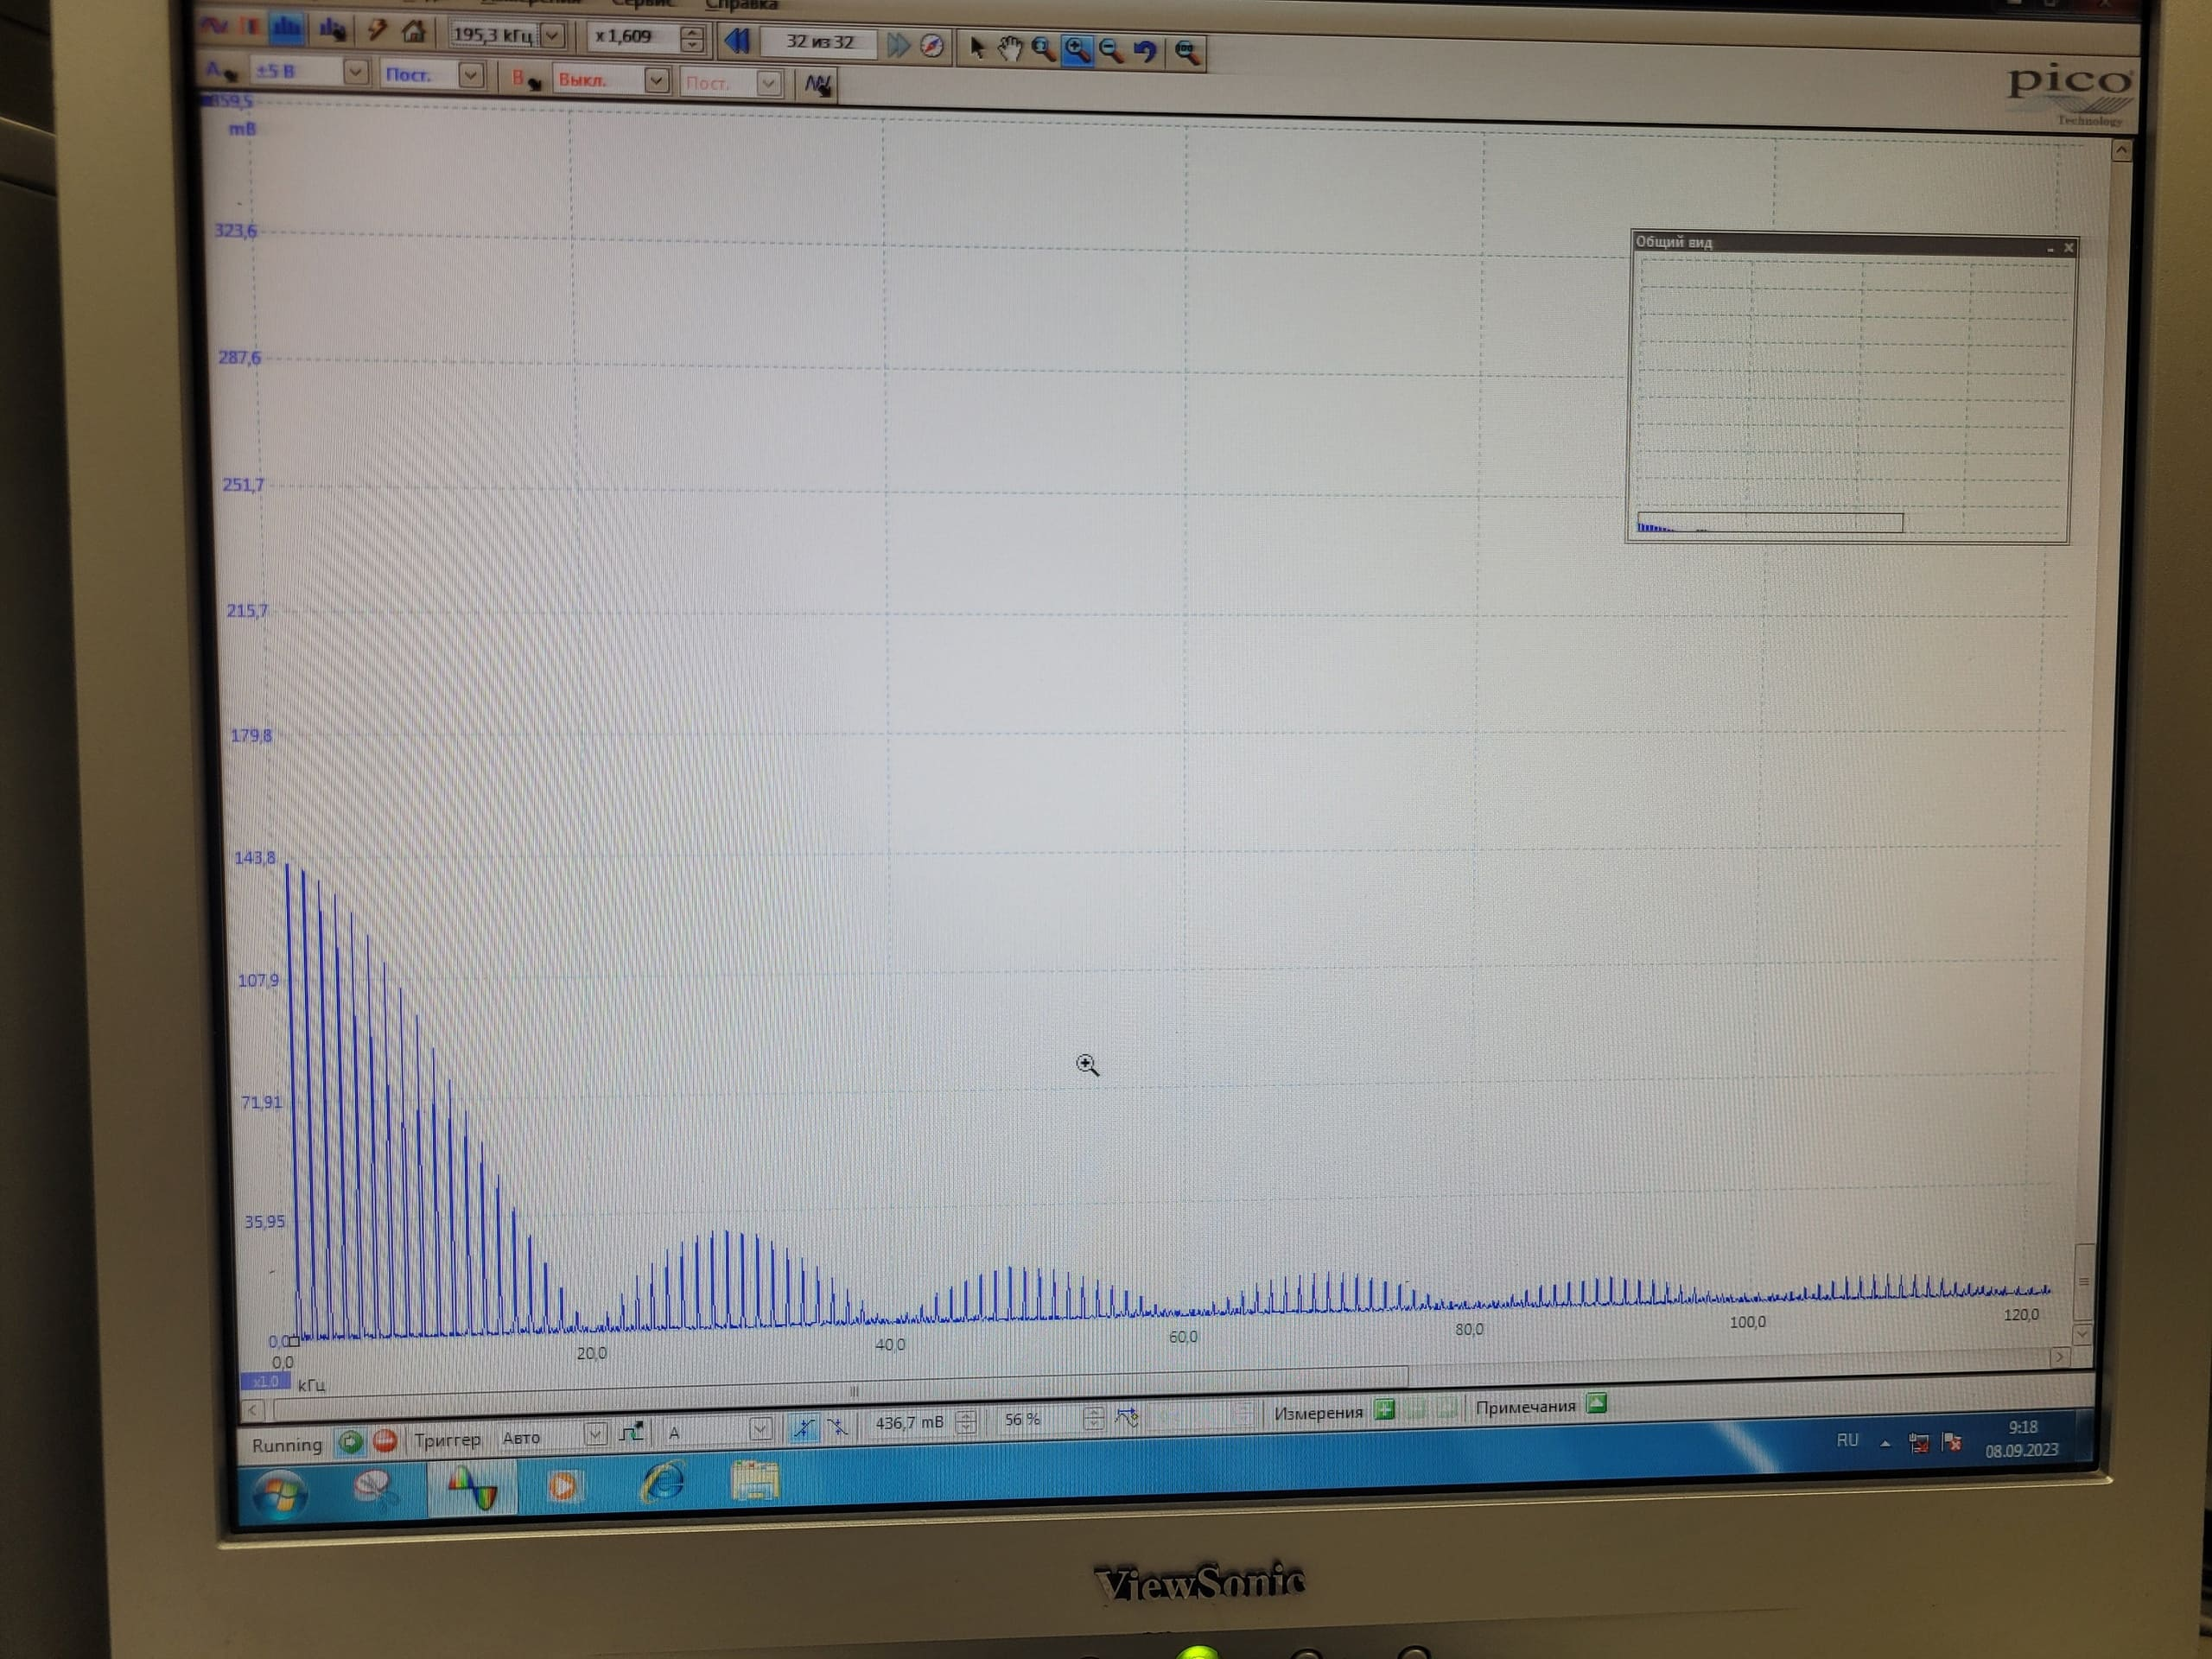
\includegraphics[width=1\linewidth]{A_1k_50.jpg}}  \\$\nu_\text{повт}$ = 1 кГц
\end{minipage}
\hfill
\begin{minipage}[h]{0.47\linewidth}
\center{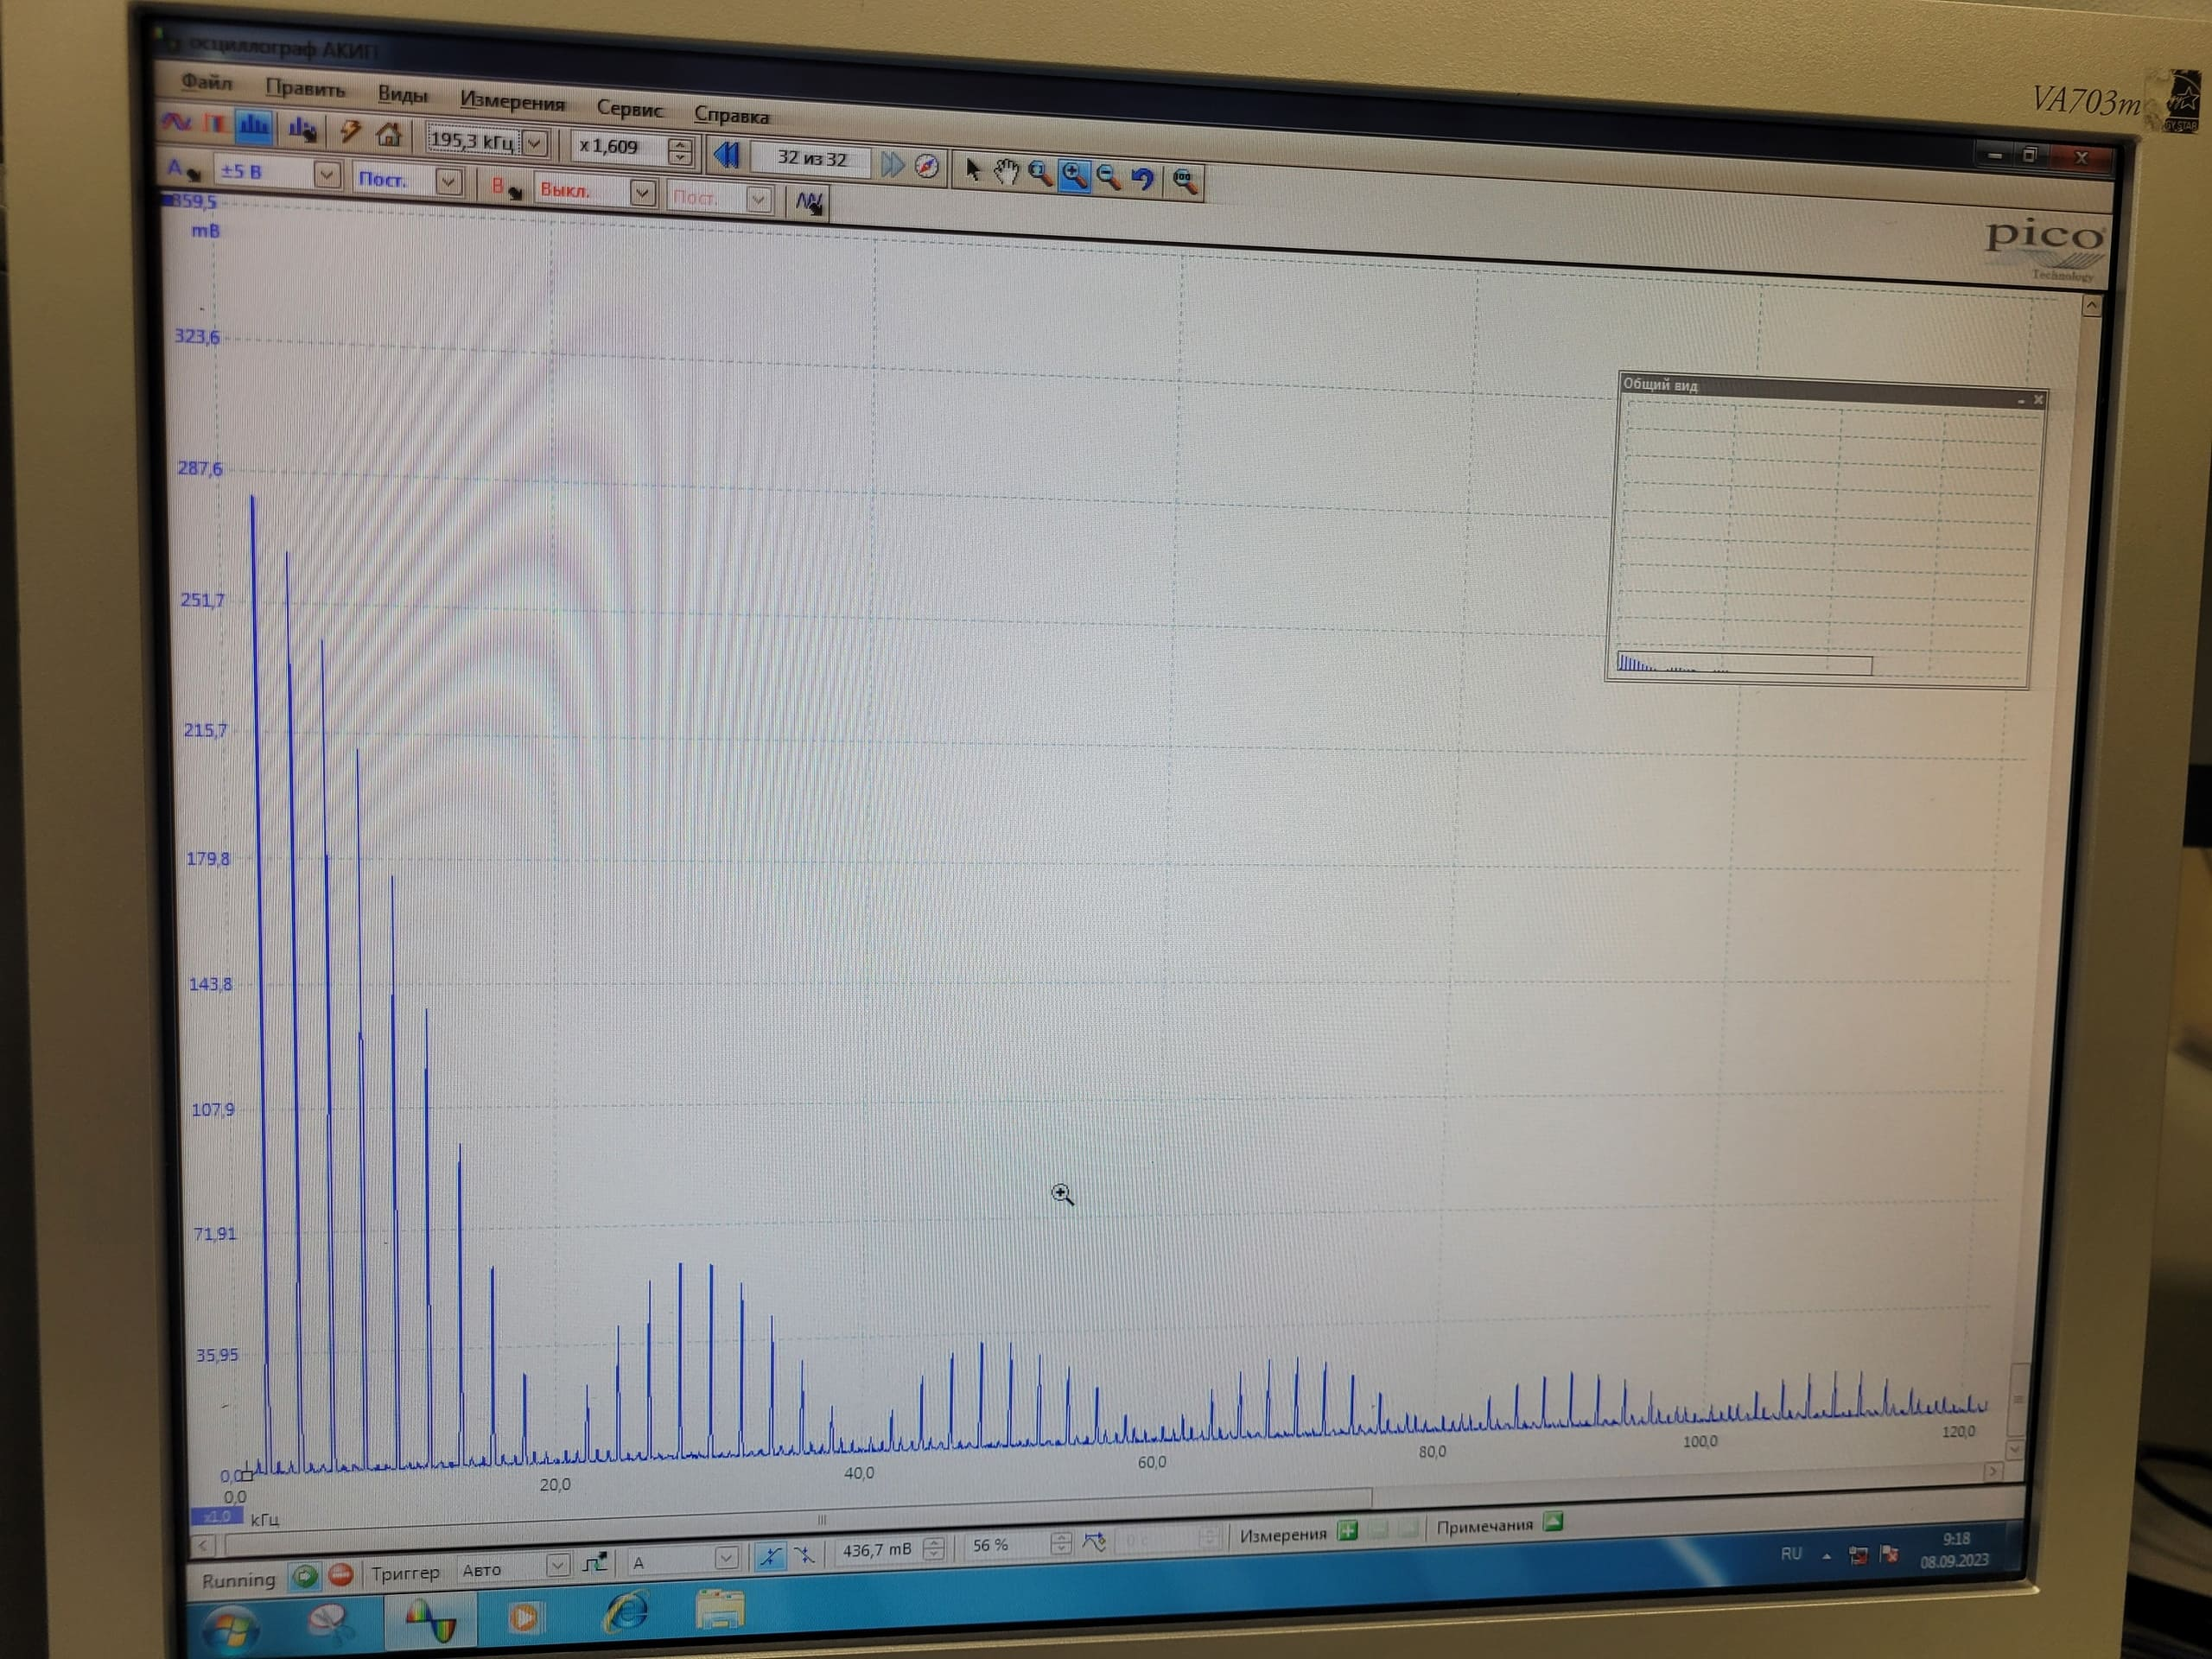
\includegraphics[width=1\linewidth]{A_2k_50.jpg}} \\$\nu_\text{повт}$ = 2 кГц
\end{minipage}
\vfill
\begin{minipage}[h]{0.47\linewidth}
\center{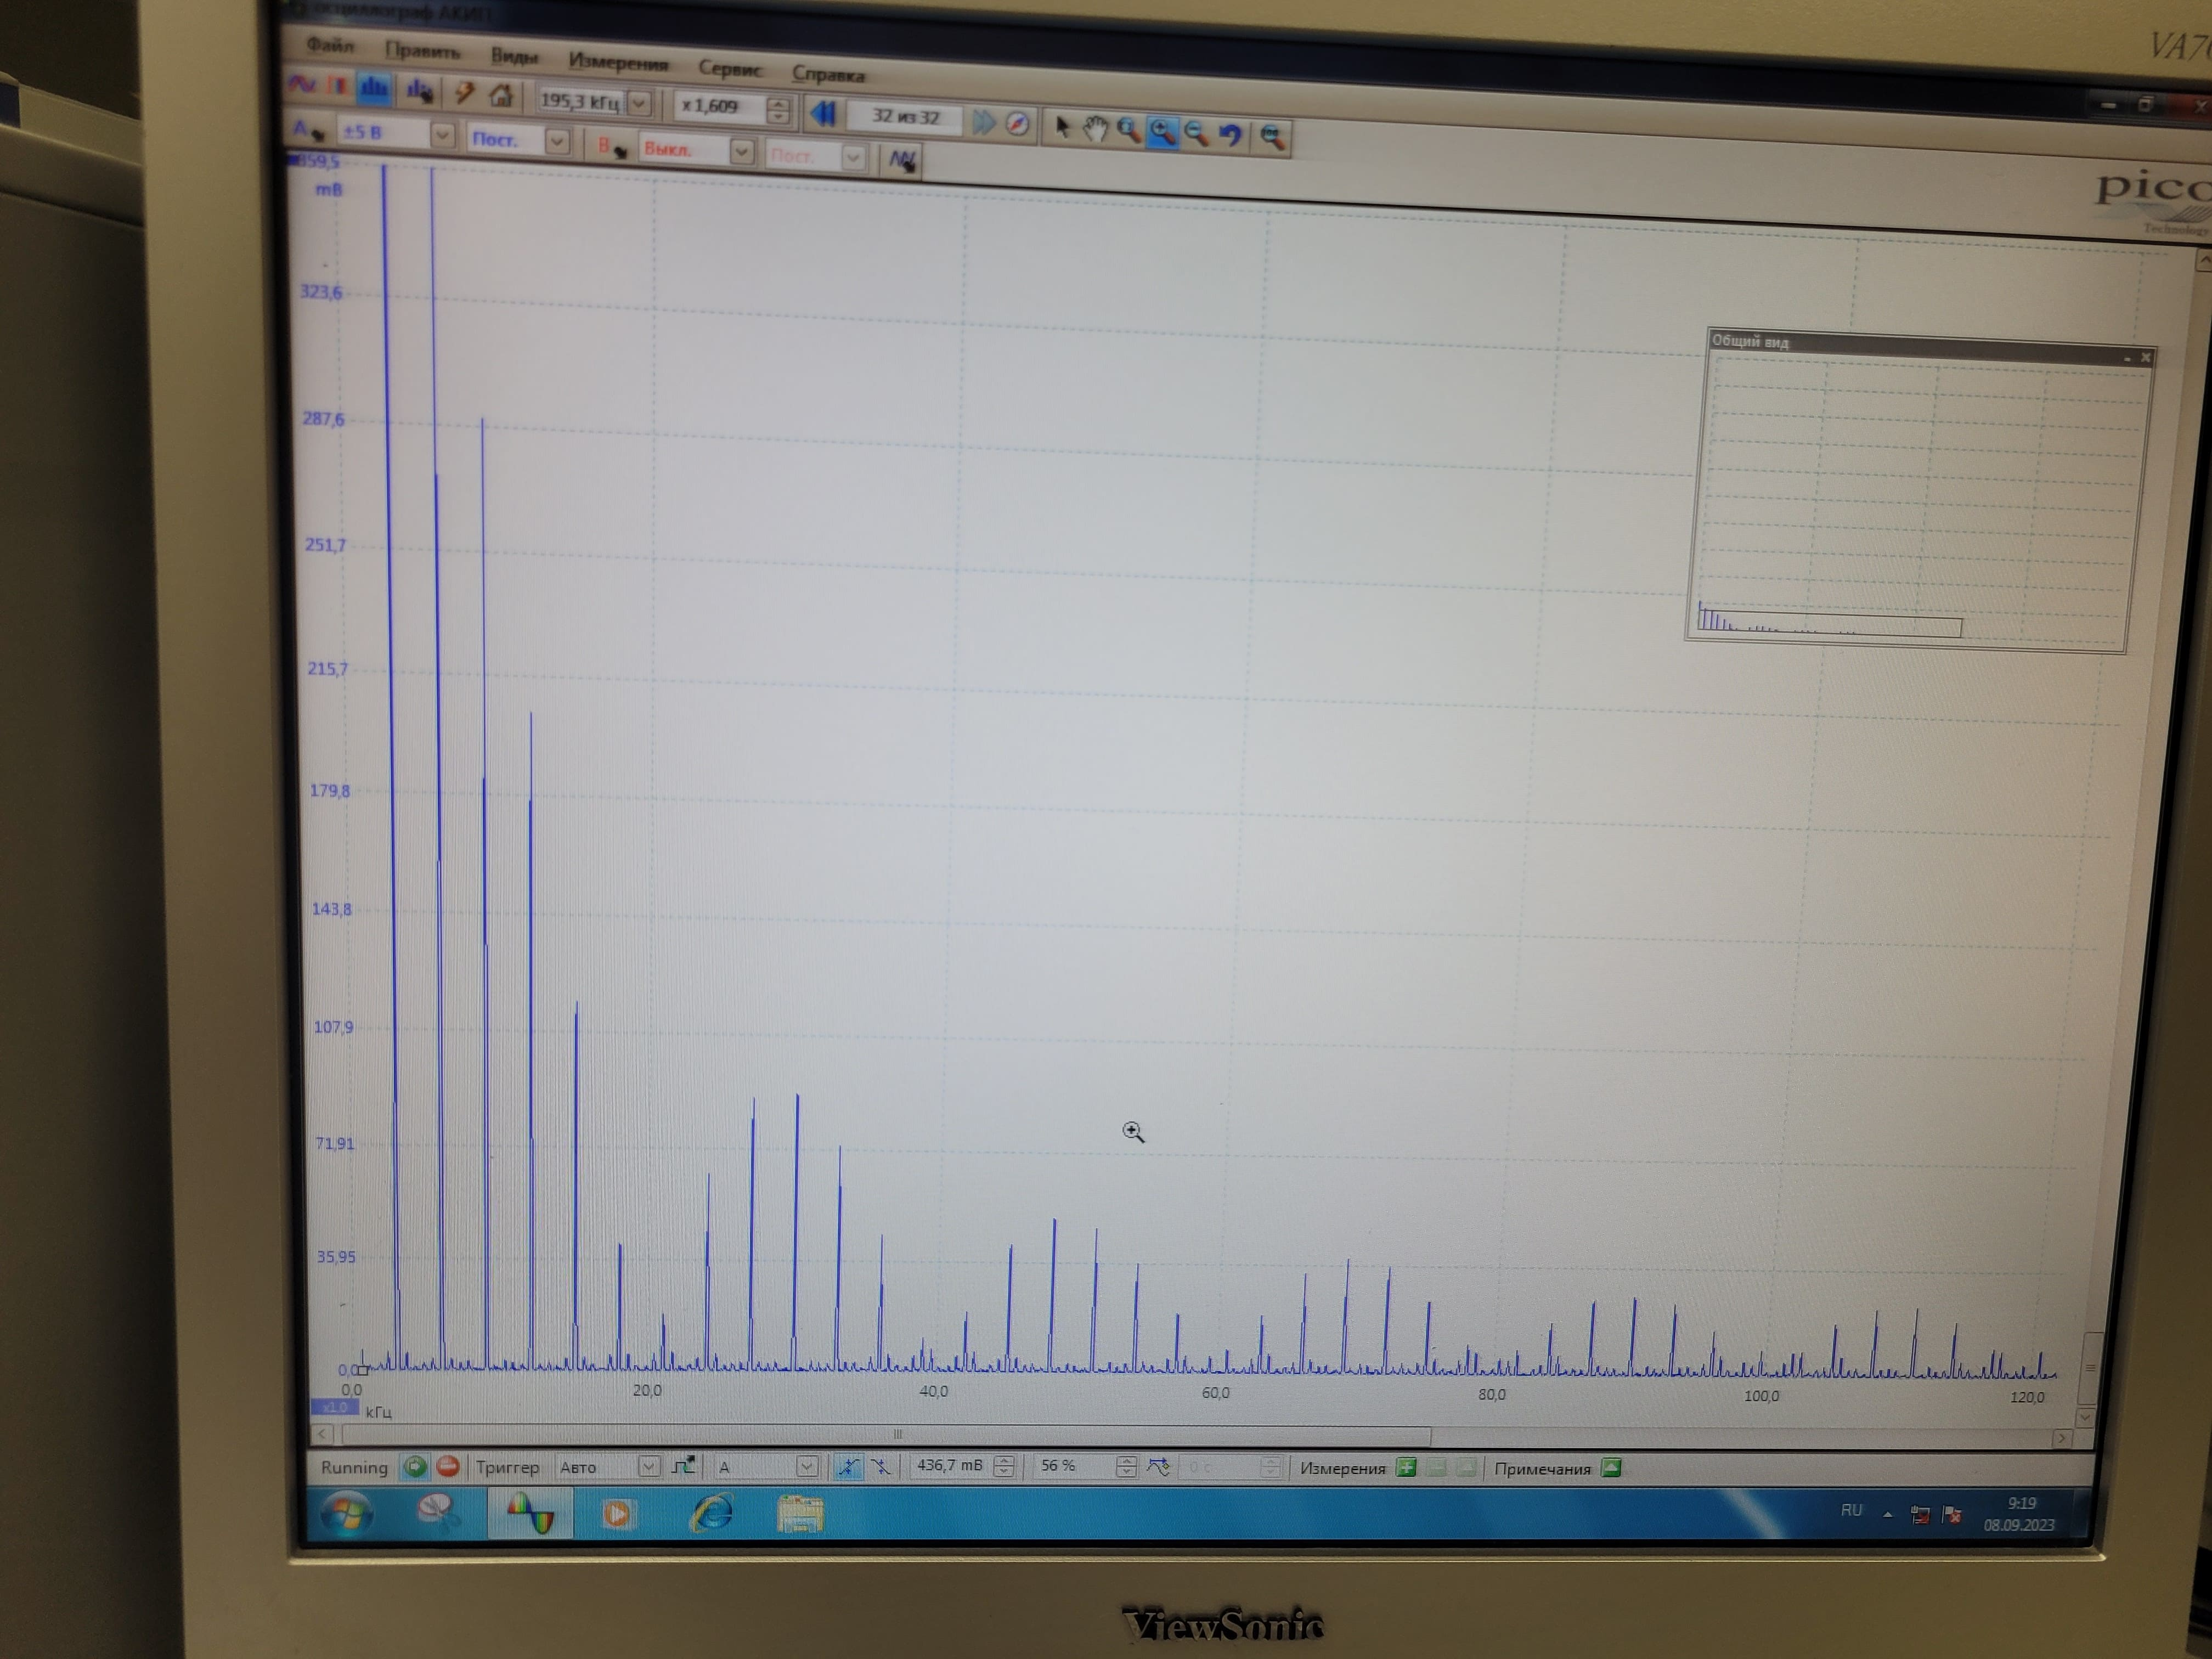
\includegraphics[width=1\linewidth]{A_3k_50.jpg}} $\nu_\text{повт}$ = 3 кГц  \\
\end{minipage}
\hfill
\begin{minipage}[h]{0.47\linewidth}
\center{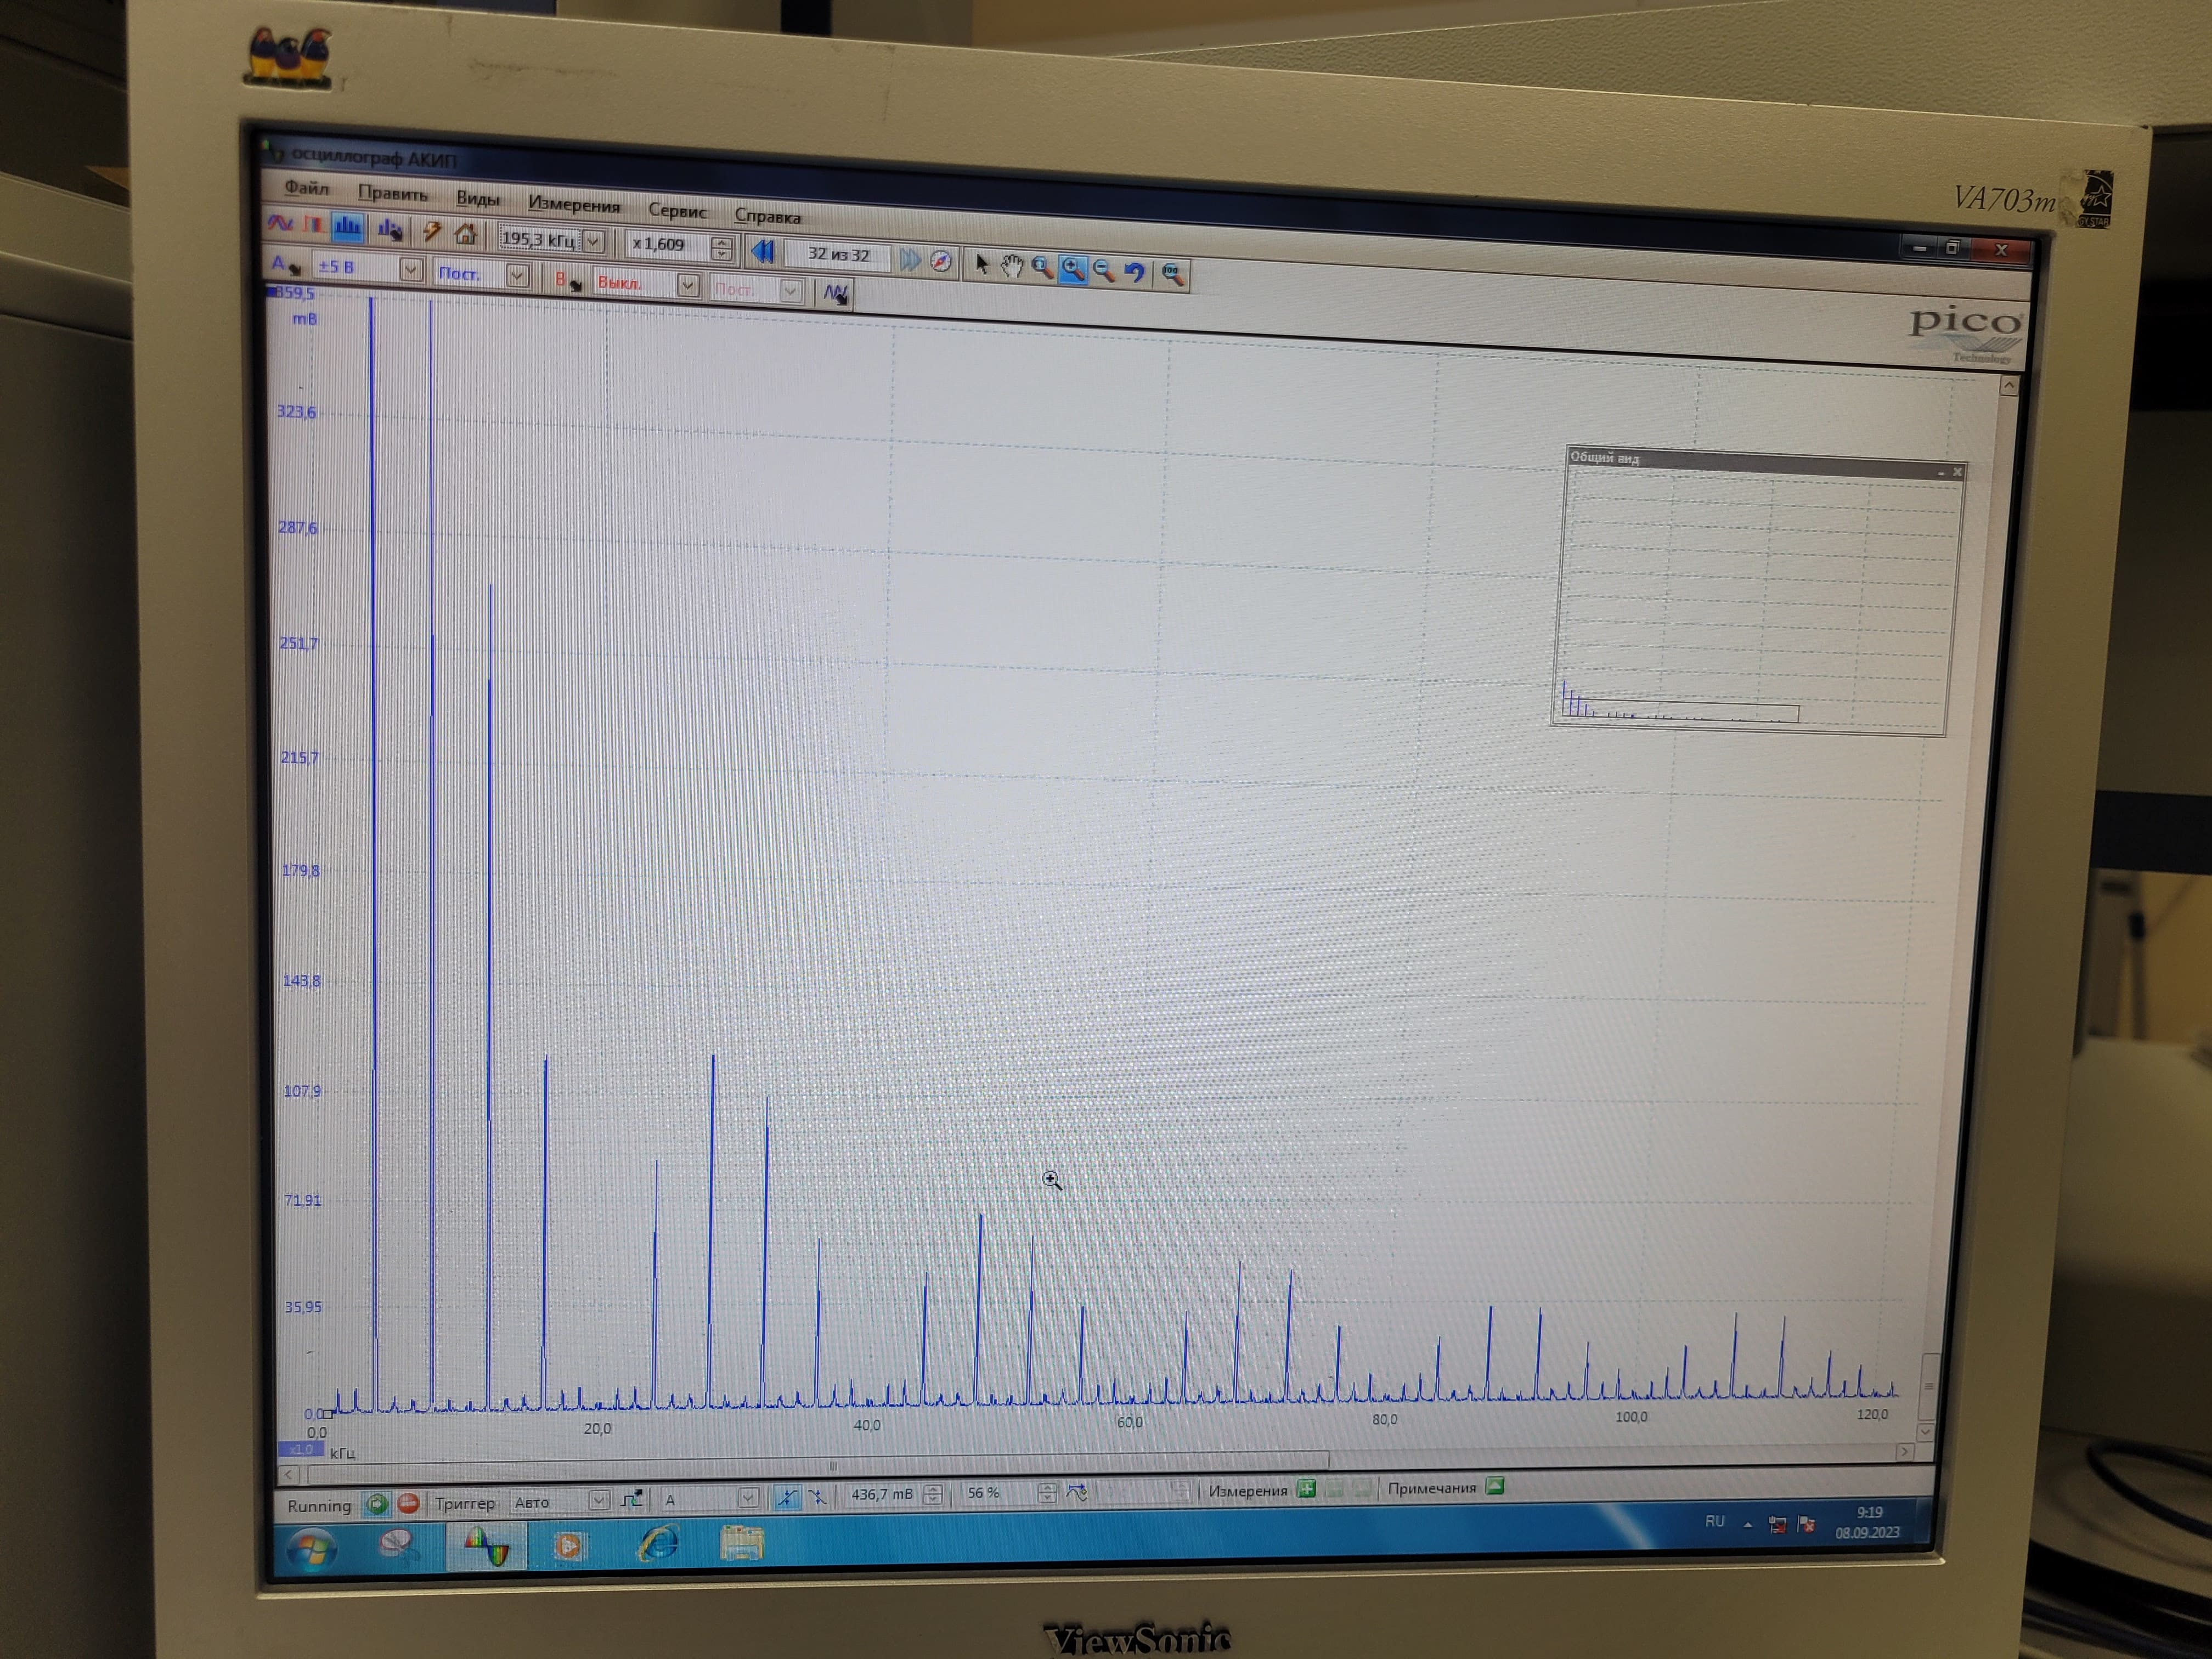
\includegraphics[width=1\linewidth]{A_4k_50.jpg}} $\nu_\text{повт}$ = 4 кГц  \\
\end{minipage}
\caption{}
\label{ris:experimentalcorrelationsignals}
\end{figure}


Как видно из графиков, при увеличении частоты повторения сигнала увеличивается расстояние между компонентами спектра.

\newpage


\textbf{б.} Изменяем $\tau$ при фиксированном $\nu_\text{повт}$ = 1 кГц и получаем:

\begin{figure}[h]
\begin{minipage}[h]{0.47\linewidth}
\center{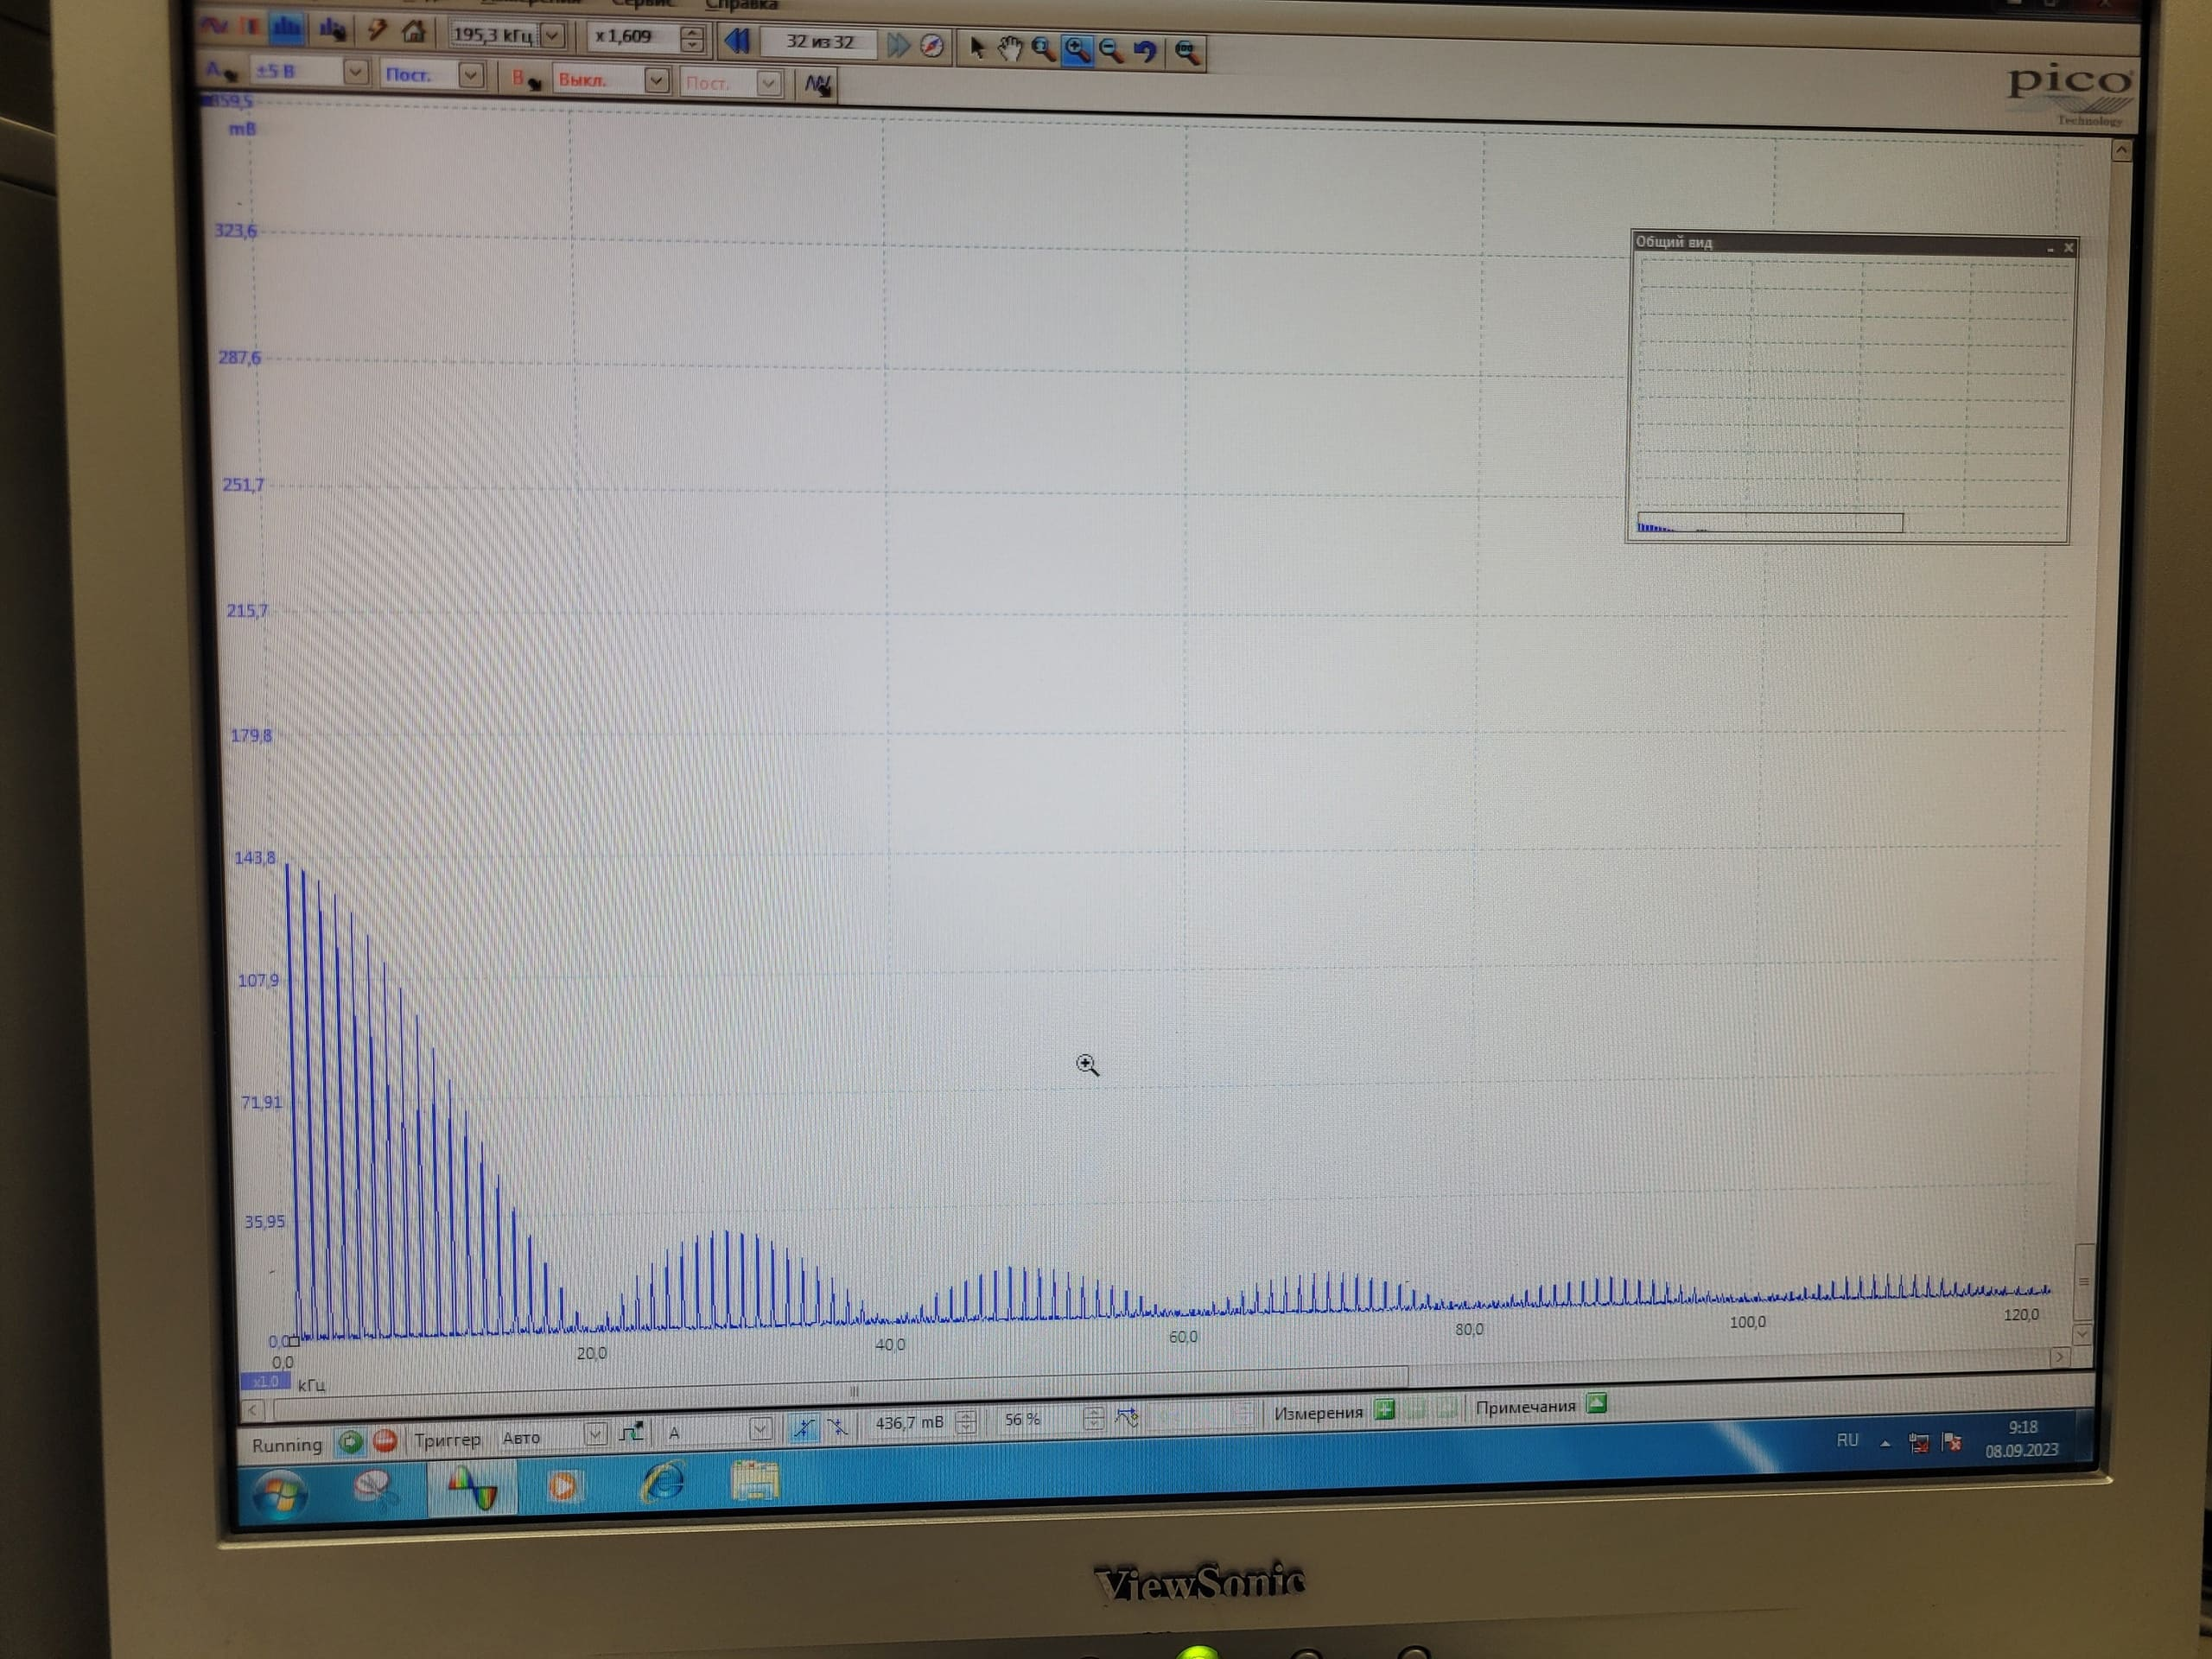
\includegraphics[width=1\linewidth]{A_1k_50.jpg}} $\tau$ = 50 мкс \\
\end{minipage}
\hfill
\begin{minipage}[h]{0.47\linewidth}
\center{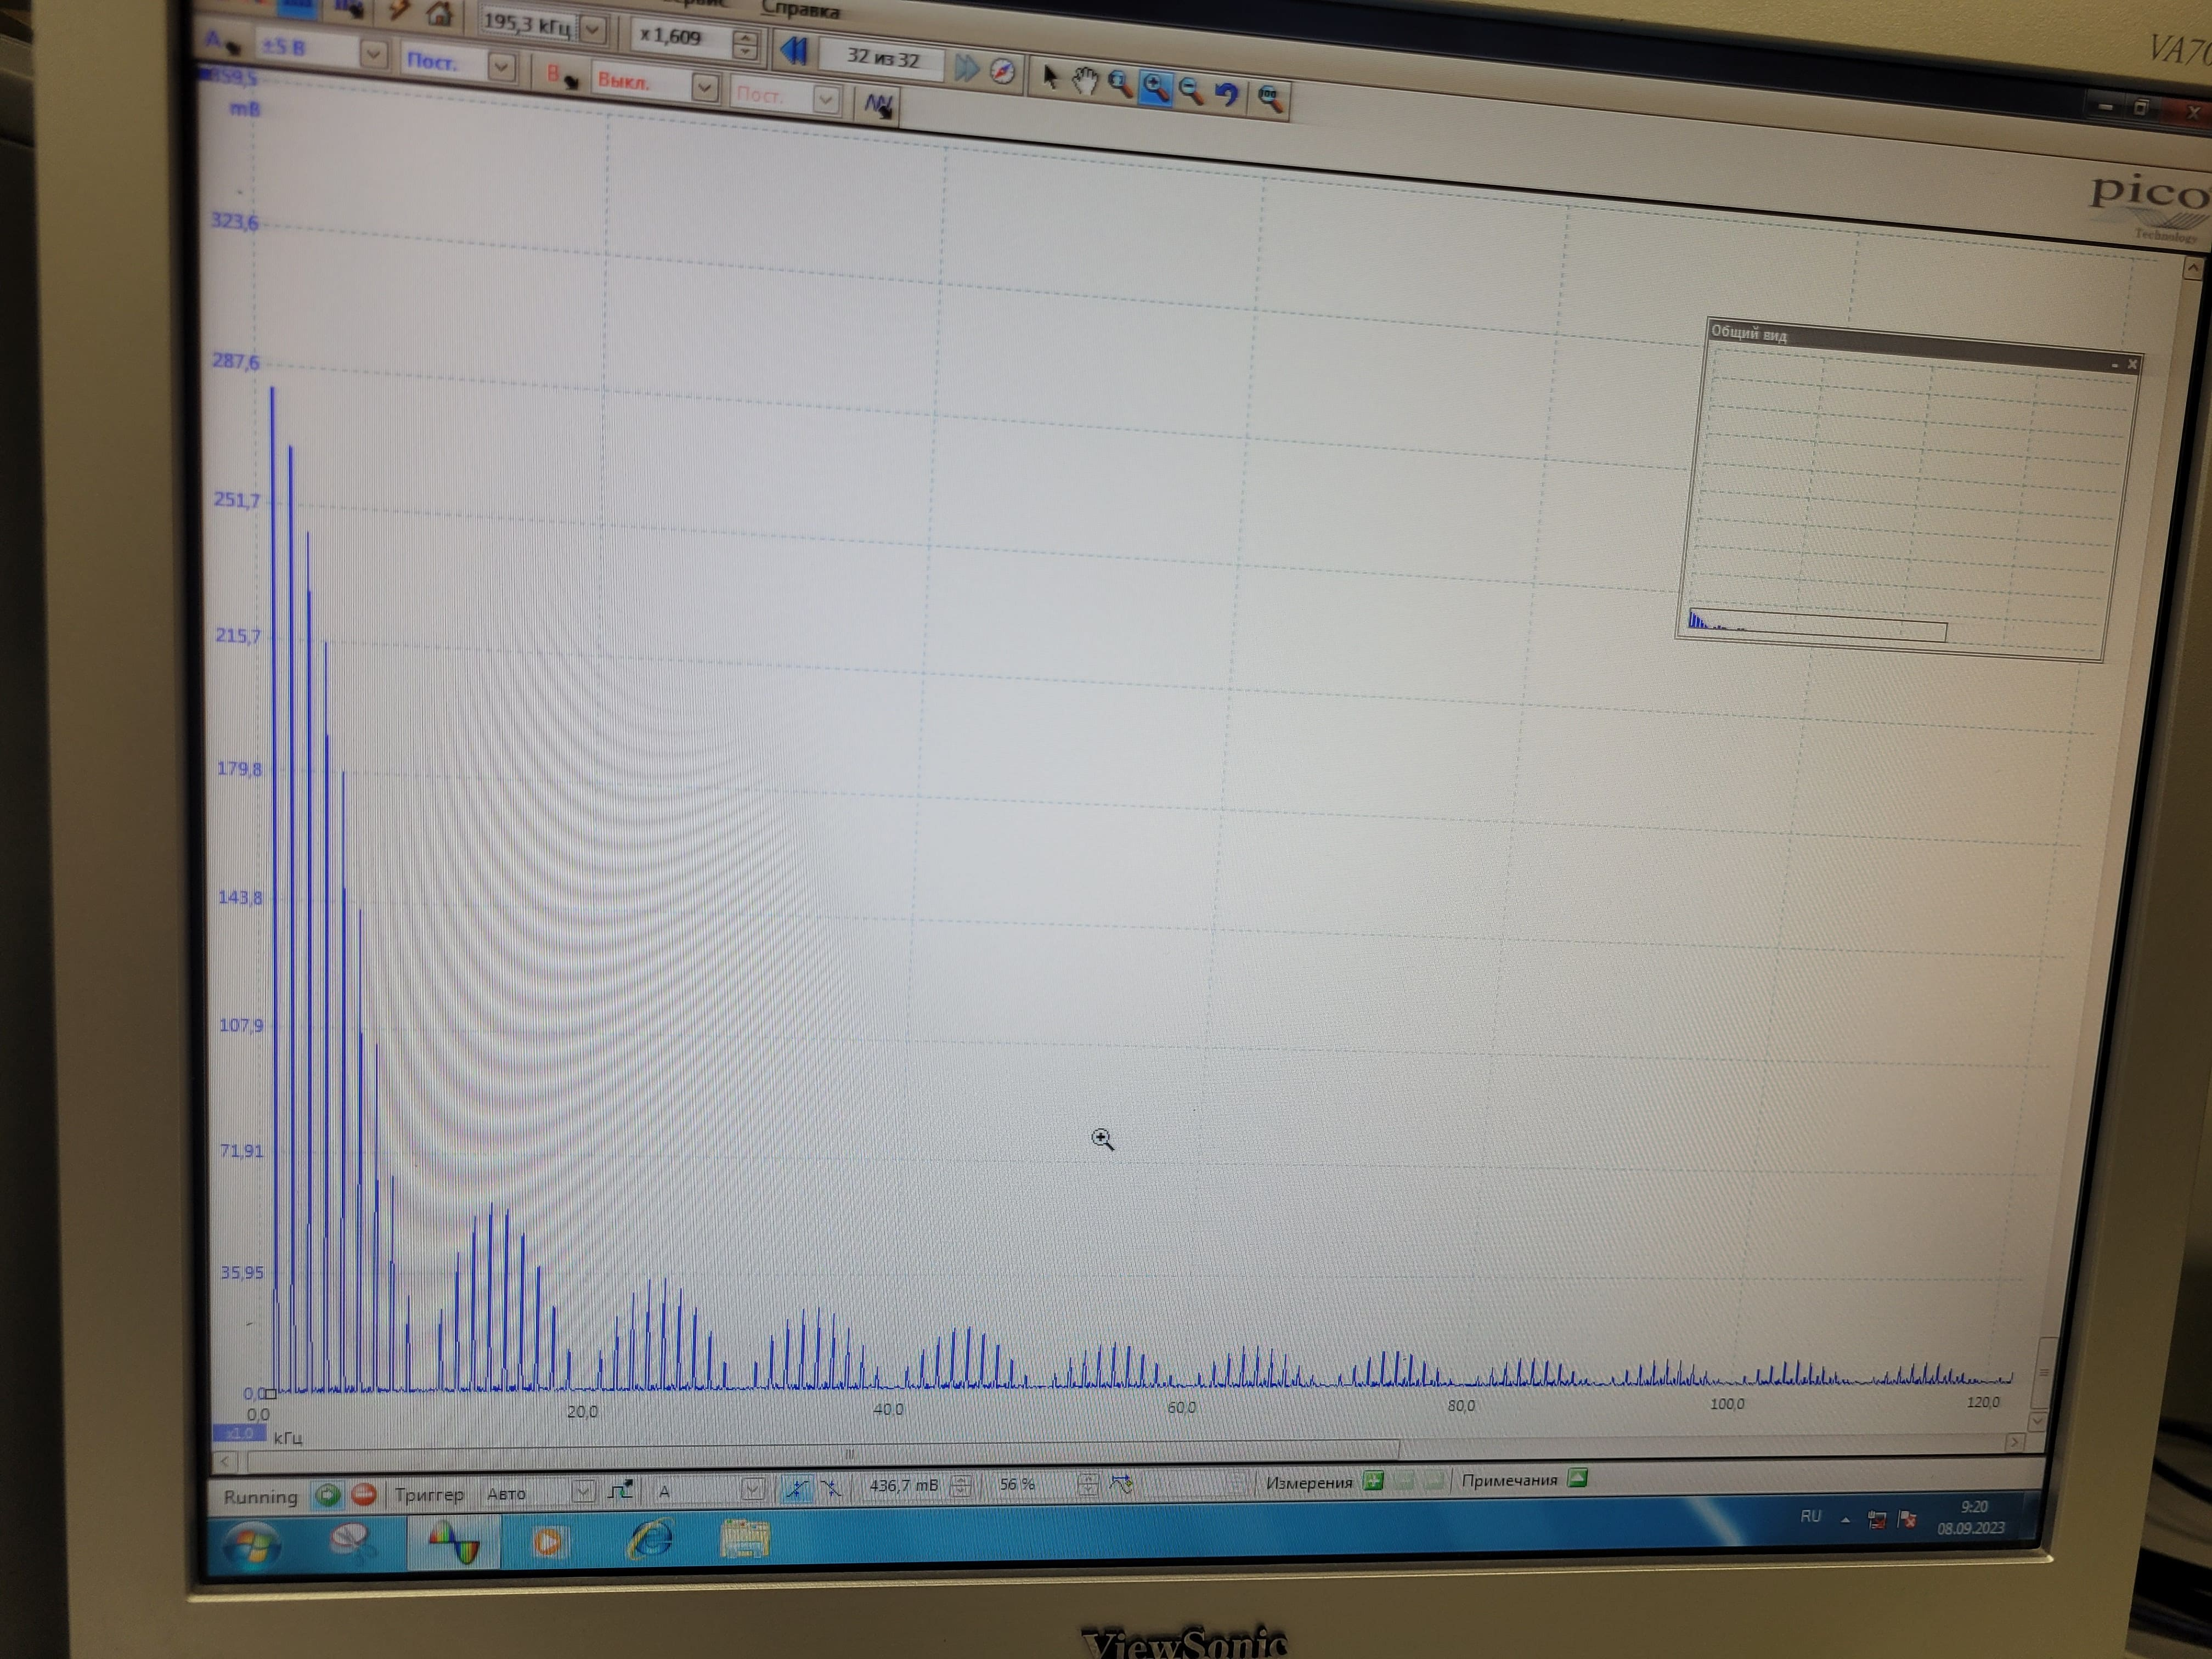
\includegraphics[width=1\linewidth]{A_1k_100.jpg}} \\ $\tau$ = 100 мкс
\end{minipage}
\vfill
\begin{minipage}[h]{0.47\linewidth}
\center{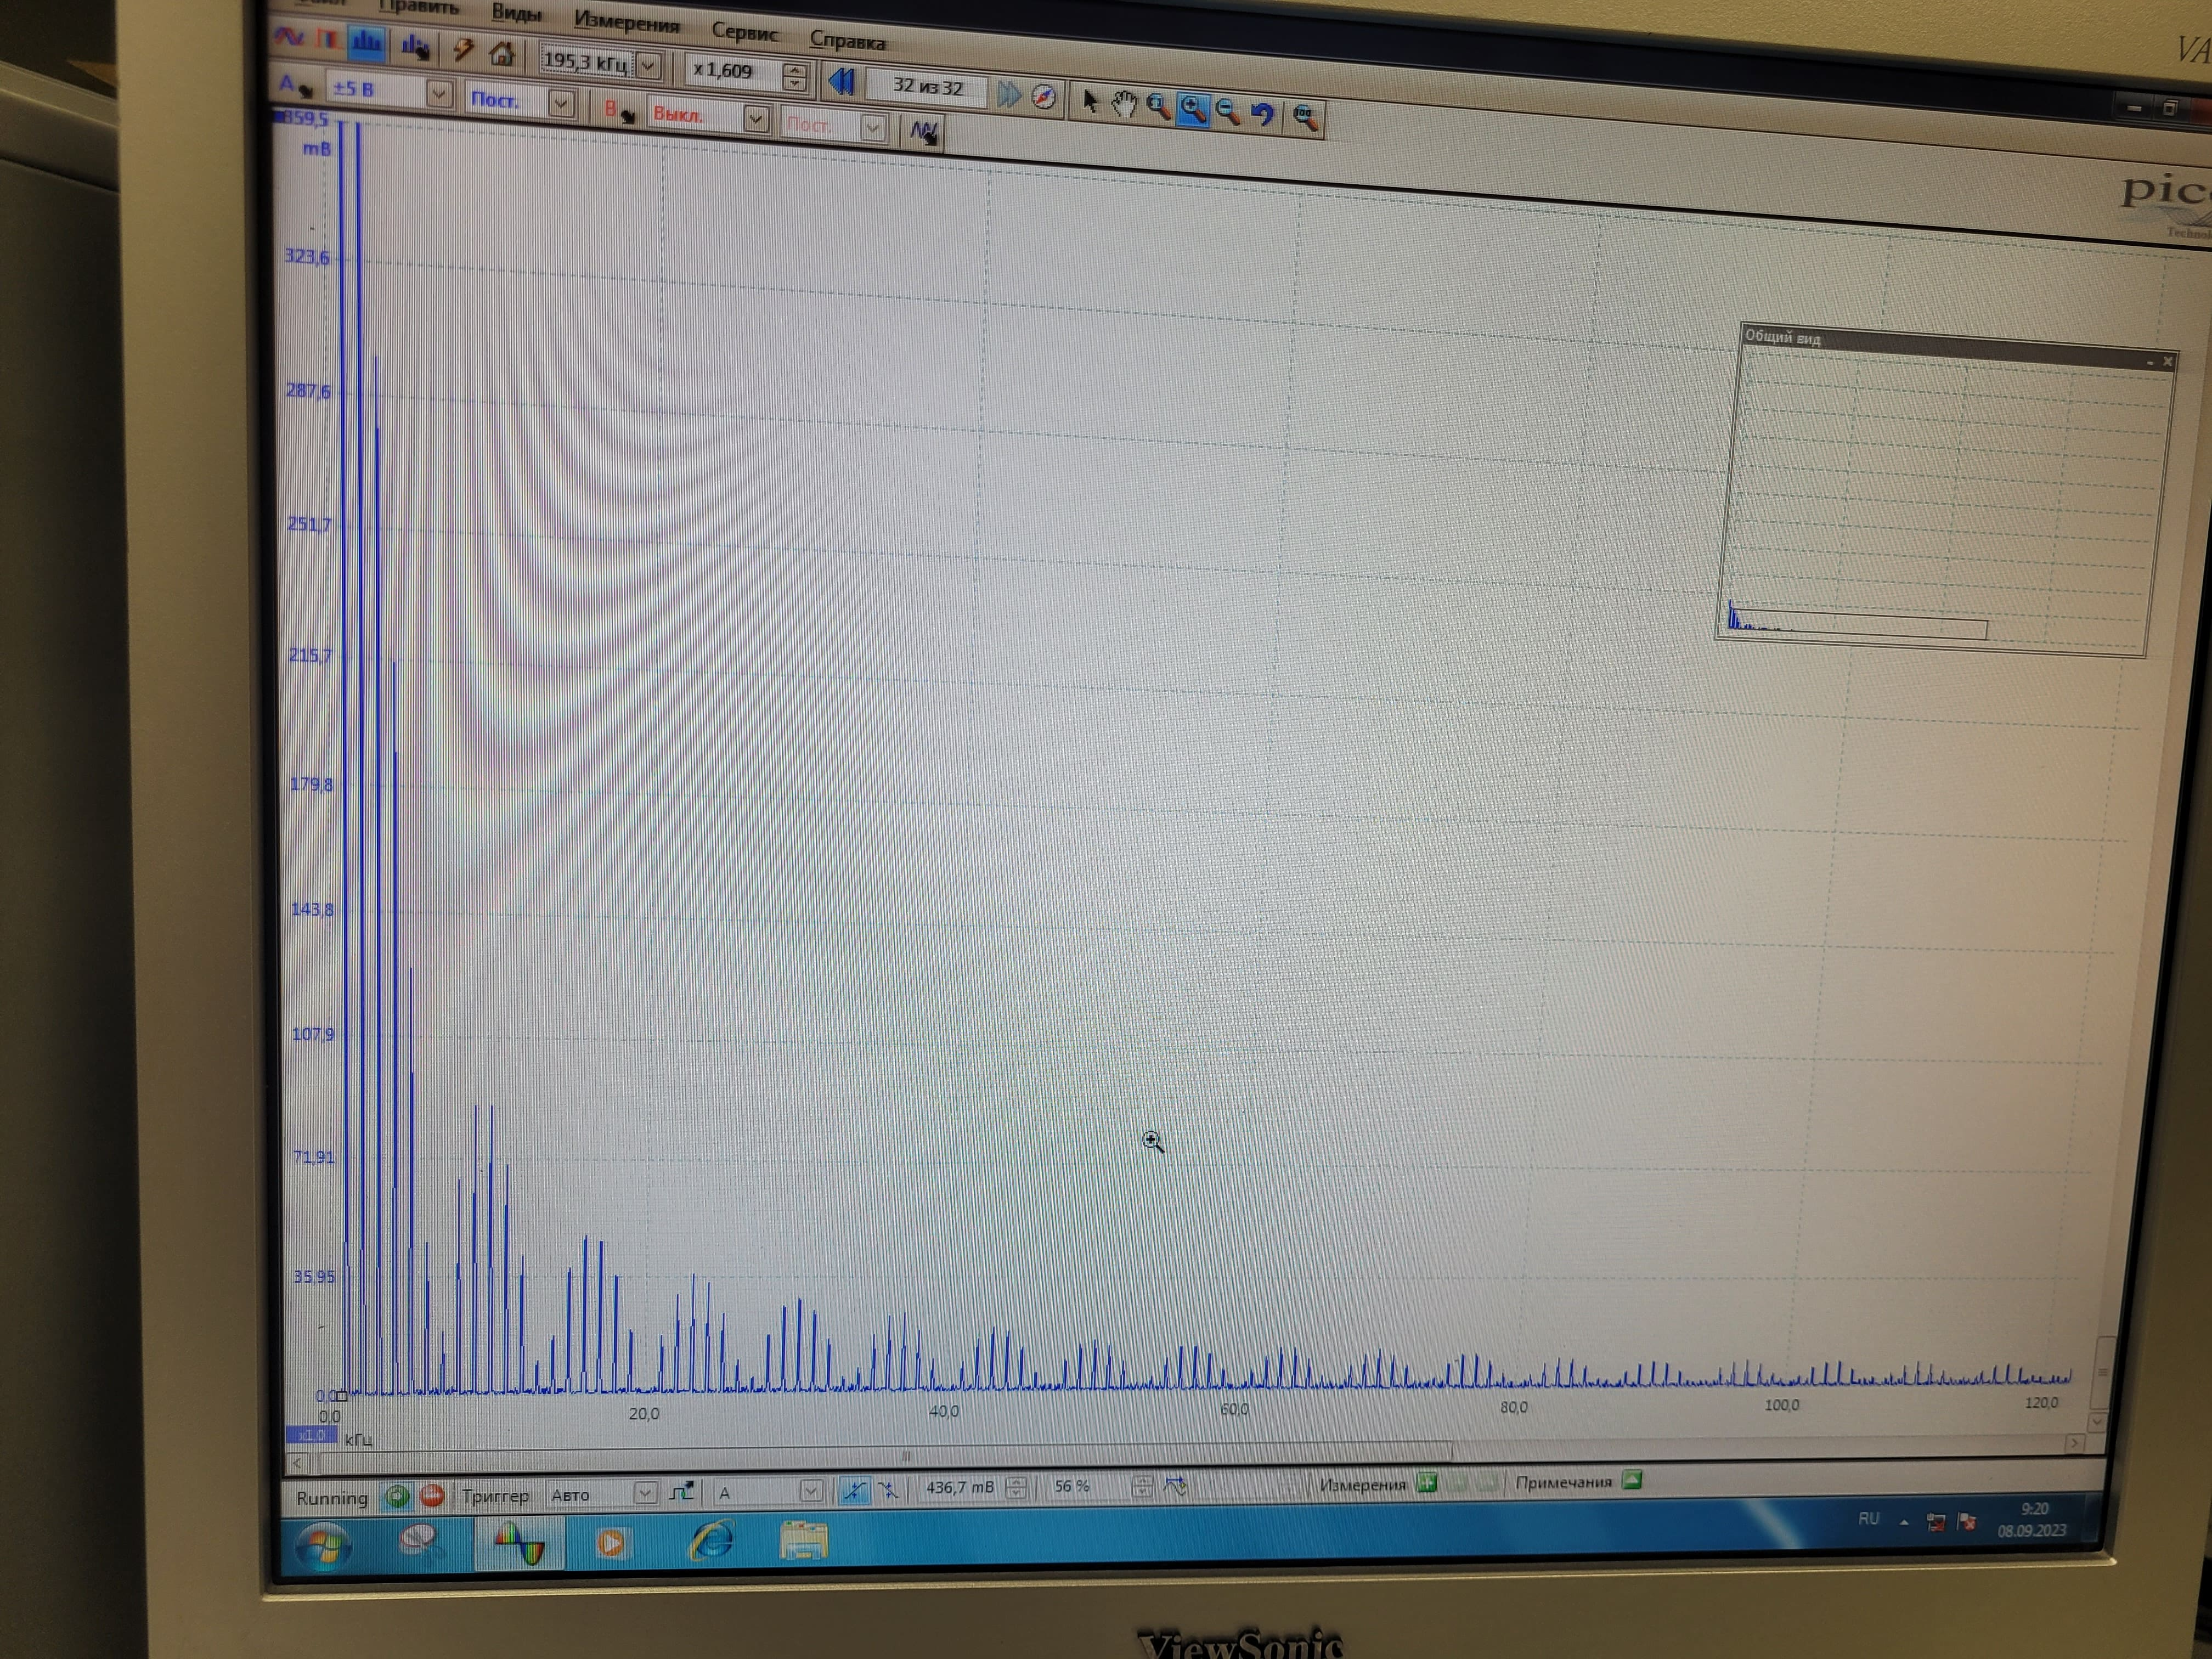
\includegraphics[width=1\linewidth]{A_1k_150.jpg}} $\tau$ = 150 мкс \\
\end{minipage}
\caption{}
\label{ris:experimentalcorrelationsignals}
\end{figure}

Как видно из графиков, при увеличении длительности сигнала уменьшается ширина спектра.

\item [\textbf{3.}] Измерим амплитуды $a_n$ и частоты $\nu_n$ спектральных гармоник при фиксированных $\nu_\text{повт}$ и $\tau$.

\begin{table}[!h]
\centering
\begin{tabular}{|l|l|l|l|l|l|l|l|l|}
\hline
$n$ гармоники & 5 & 7 & 9 & 11 & 13 & 15 & 17 & 19 \\ \hline
$\nu_n^\text{эксп}$, кГц & 5.078 & 7.092 & 8.904 & 11.12 & 13.03 & 15.15 & 16.76 & 19.17 \\ \hline
$\nu_n^\text{теор}$, кГц & 5 & 7 & 9 & 11 & 13 & 15 & 17 & 19 \\ \hline
$|a_n|^\text{эксп}$, мВ & 125.9 & 112.3 & 94.73 & 73.98 & 54.58 & 37.44 & 20.75 & 4.962 \\ \hline
$|a_n/a_1|_\text{эксп}$ & 0.876 & 0.781 & 0.659 & 0.515 & 0.380 & 0.261 & 0.144 & 0.034 \\ \hline
$|a_n/a_1|_\text{теор}$ & 0.904 & 0.814 & 0.702 & 0.574 & 0.438 & 0.301 & 0.171 & 0.052 \\ \hline
\end{tabular}
\end{table}

Здесь $a_1$ = 143.8 мВ.
$$\nu_n^\text{теор} = \frac{n}{T}$$
$$|a_n|_\text{теор} = \frac{|\text{sin}\frac{\pi n \tau}{T}|}{\pi n}$$

\item[\textbf{4.}] Зафиксируем период повторения прямоугольного сигнала $T = 1 \text{мс}$, $\nu_\text{повт} = 1\text{кГц}$. Изменяя длительность импульса $\tau$ в диапазоне от
$\tau=T/50$ до $\tau=T/5$, измерим полную ширину спектра сигнала $\Delta \nu$ — от центра спектра ($\nu = 0$) до гармоники с нулевой амплитудой $a_n \approx 0$ и установим зависимость между $\Delta \nu$ и $\tau$, полученную из формулы \ref{eq5}.

\begin{table}[h!]
    \centering
    \begin{tabular}{|c|c|c|c|c|c|c|c|}
\hline
$\tau$, мкс & 20 & 25 & 40 & 50 & 100 & 150 & 200 \\ \hline
$\Delta \nu$, кГц & 49.68 & 39.71 & 24.61 & 19.98 & 9.91 & 6.84 & 4.93 \\ \hline
$1/\tau \cdot 10^3$, с$^{-1}$ & 50 & 40 & 25 & 20 & 10 & 7 & 5 \\ \hline
\end{tabular}
    \caption{Исследование зависимости $\Delta \nu$ и $\tau$}
    \label{table2}
\end{table}
Построим график $\Delta\nu\left(\frac{1}{\tau}\right)$. Используя МНК, получим $k=0.994\pm0,002$, откуда с хорошей точностью можем заключить, что $\Delta\nu\frac{1}{\tau}=1$, что экспериментально доказывает соотношение неопределённостей. График приведён на рис.12
\begin{figure}[h]
    \centering
    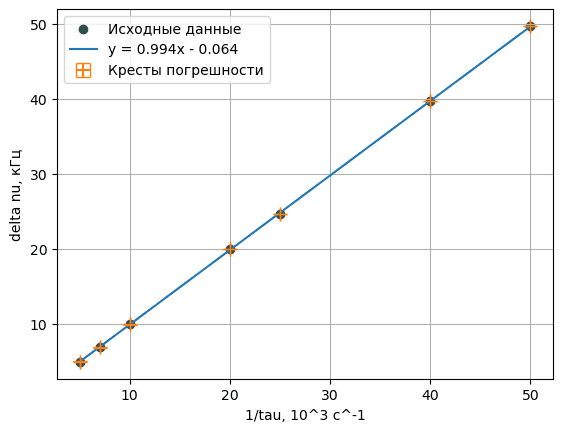
\includegraphics[width=0.7\linewidth]{grafic1.png}
    \caption{Зависимость $\Delta \nu$ от $1/\tau$}
    \label{grafic1}
\end{figure}

\item[\textbf{5.}]
Зафиксируем длительность импульса прямоугольного сигнала $\tau = 100 \text{мкс}$. Изменяя период повторения $T$ в диапазоне от $2\tau$ до $50\tau$ измерим расстояния $\delta\nu = \nu_{n+1} - \nu_n$ между соседними гармониками спектра.
\begin{table}[h!]
    \centering
    \begin{tabular}{|c|c|c|c|c|c|c|}
\hline
$\nu$, кГц & 5 & 2 & 1 & 0.5 & 0.25 & 0.1 \\ \hline
$\delta \nu$, кГц & 5.036 & 1.927 & 1.008 & 0.510 & 0.253 & 0.206 \\ \hline
\end{tabular}
    \caption{Зависимость $\delta \nu$ от $1/T$}
    \label{table3}
\end{table}

\newpage

\begin{figure}[h]
    \centering
    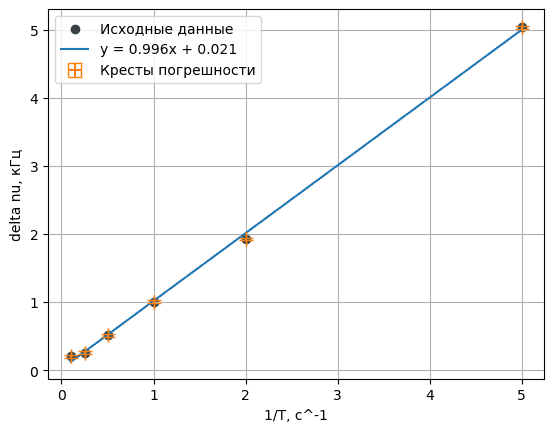
\includegraphics[width=0.7\linewidth]{grafic2.png}
    \caption{Зависимость $\delta \nu$ от $1/T$}
    \label{grafic2}
\end{figure}
Построим график $\delta\nu\left(\frac{1}{T}\right)$. Используя МНК, получим $k=0.996\pm0,013$, что экспериментально доказывает соотношение неопределённостей. График приведён на рис.13.
\end{enumerate}


\newpage

\subsection*{Б. Наблюдение спектра периодической последовательности цугов}

\begin{enumerate}
\item [\textbf{1.}] Настраиваем генератор на периодичные импульсы синусоидальной формы (цугов) с несущей частотой $\nu_0$ = 50 кГц, частотой повторения $\nu_\text{повт}$ = 1 кГц, число периодов синусоиды в одном импульсе $N$ = 5 (что соответствует длительности импульса $\tau$ = $N/\nu_o$ = 100 мкс).

\item [\textbf{2.}] Получаем на экране спектр (Преобразование Фурье) сигнала.

\textbf{a.} Изменяем $N$ при фиксированных $\nu_0$ = 50 кГц и $\nu_\text{повт}$ = 1 кГц:

\begin{figure}[h]
\begin{minipage}[h]{0.47\linewidth}
\center{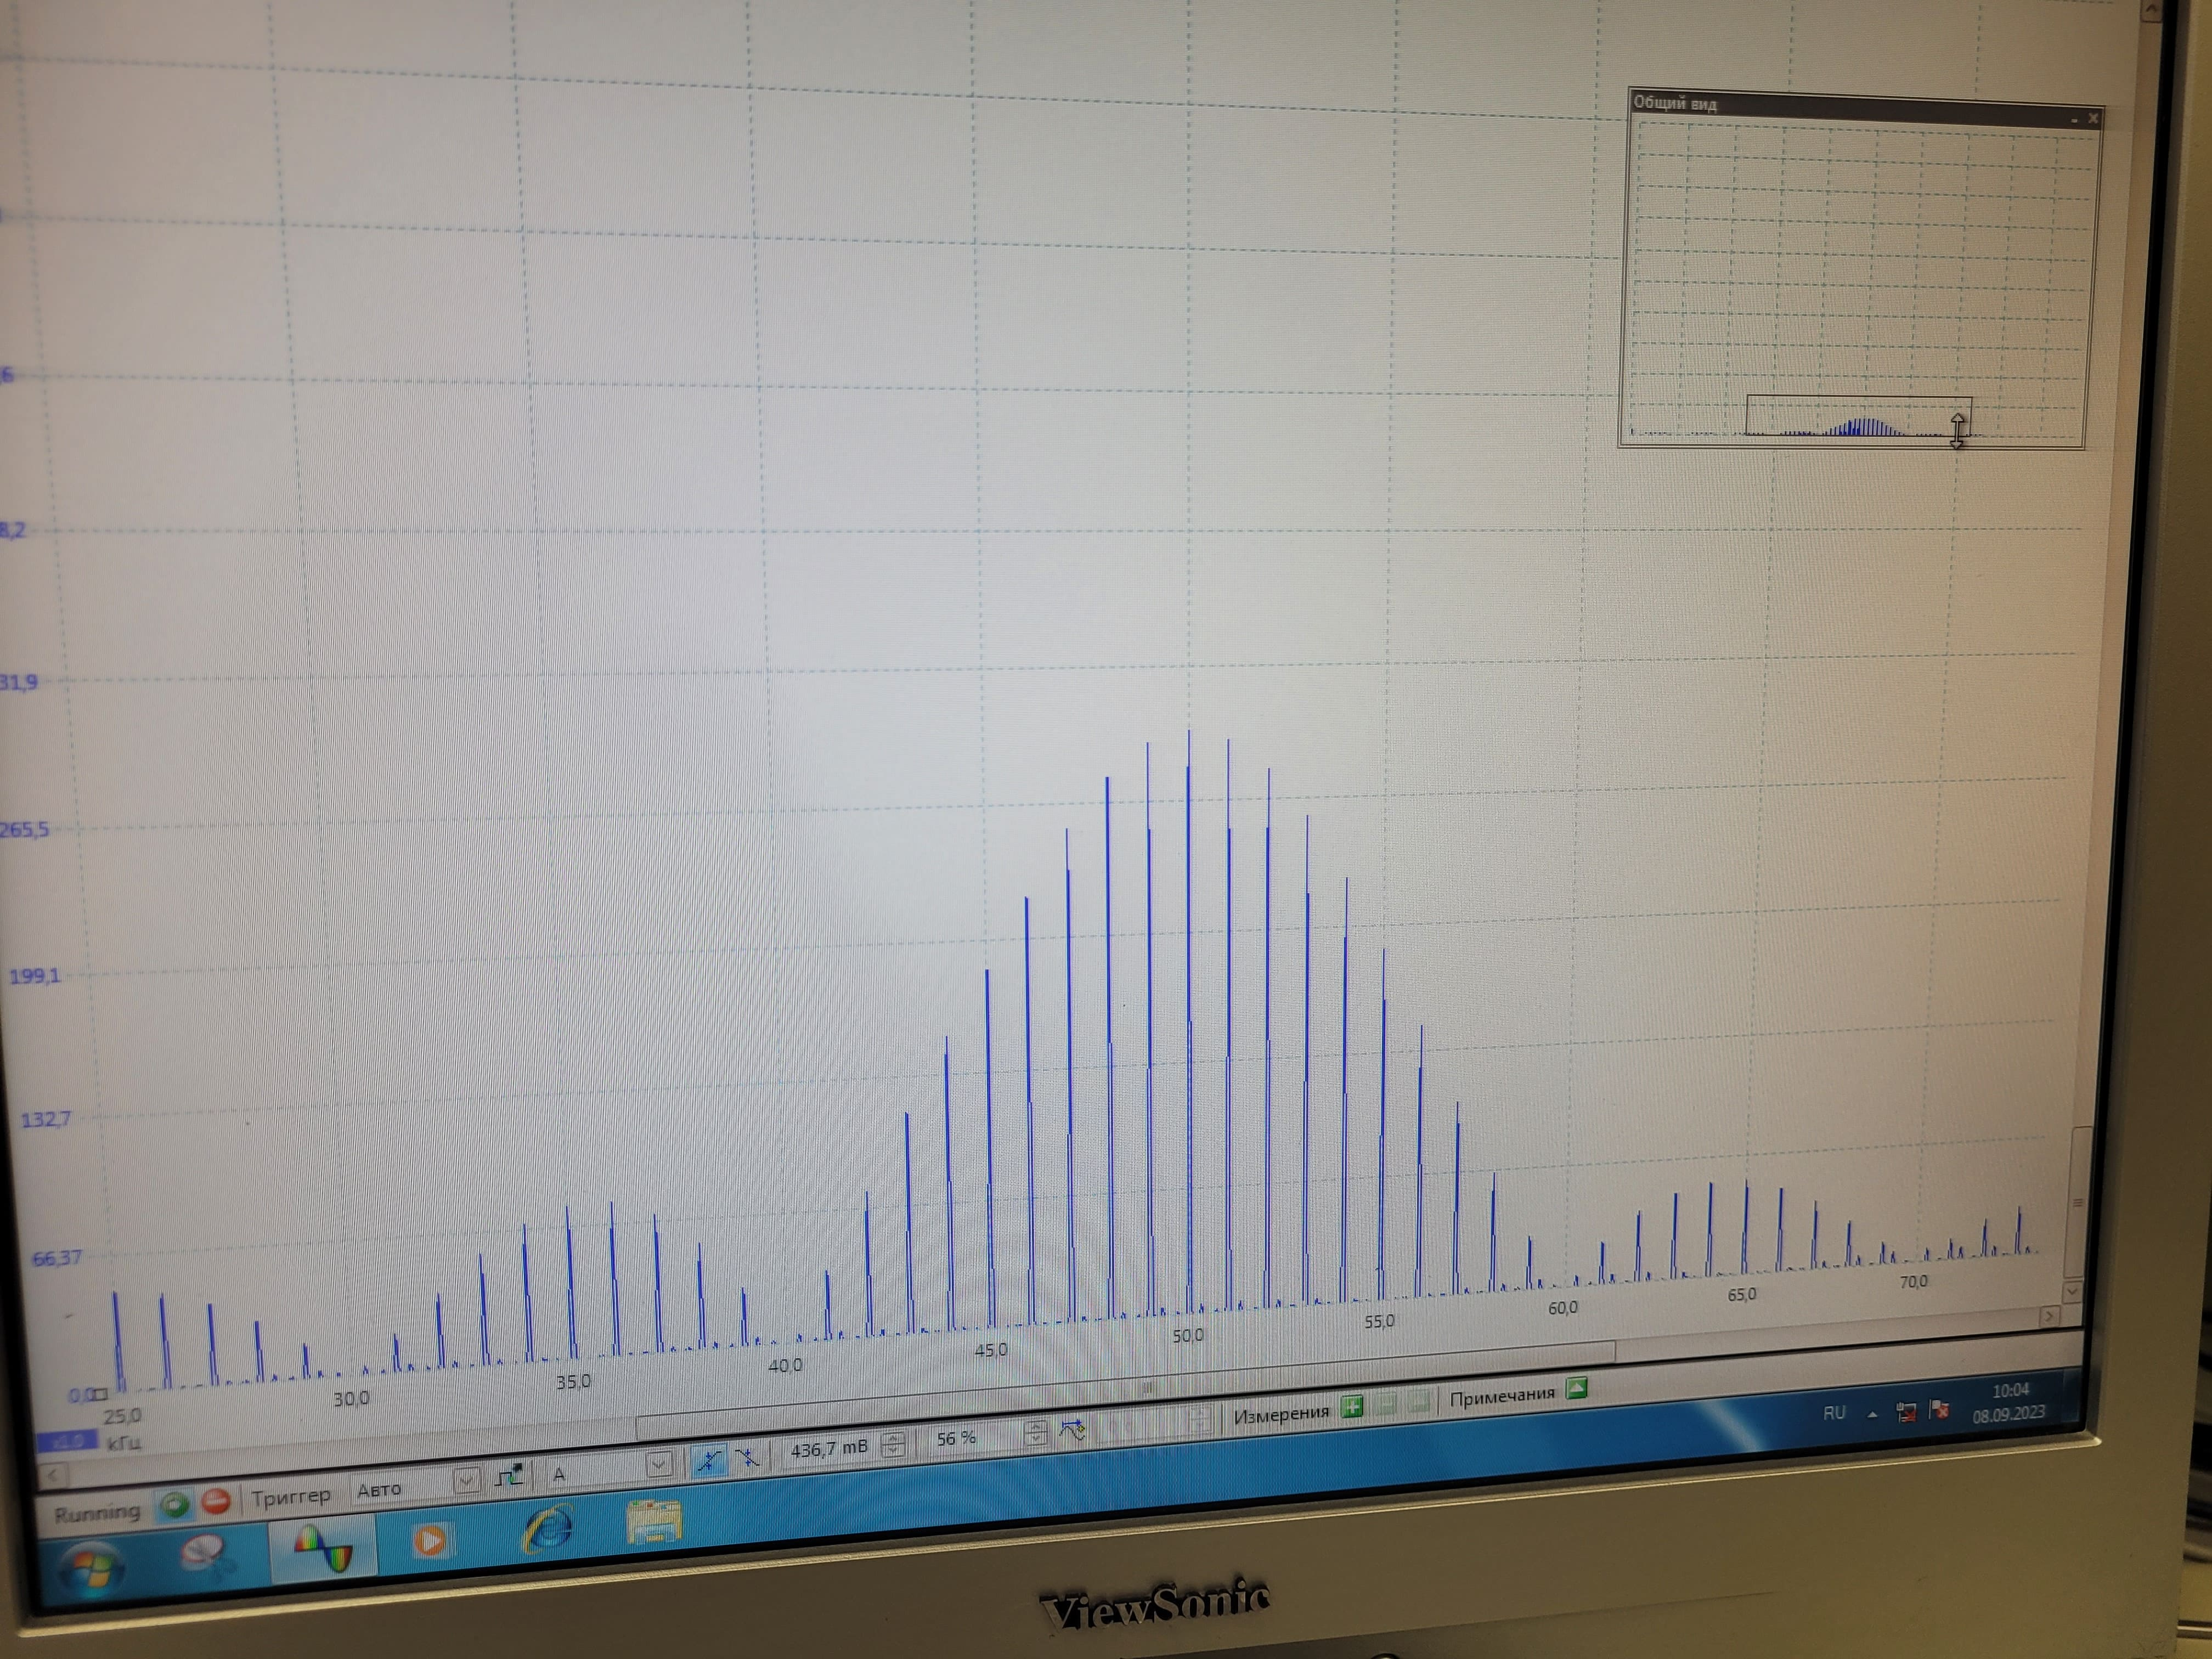
\includegraphics[width=1\linewidth]{B_50k_1k_5.jpg}} N=5, $\delta \nu$ = 1 кГц, $\Delta \nu$ = 10 кГц\\
\end{minipage}
\hfill
\begin{minipage}[h]{0.47\linewidth}
\center{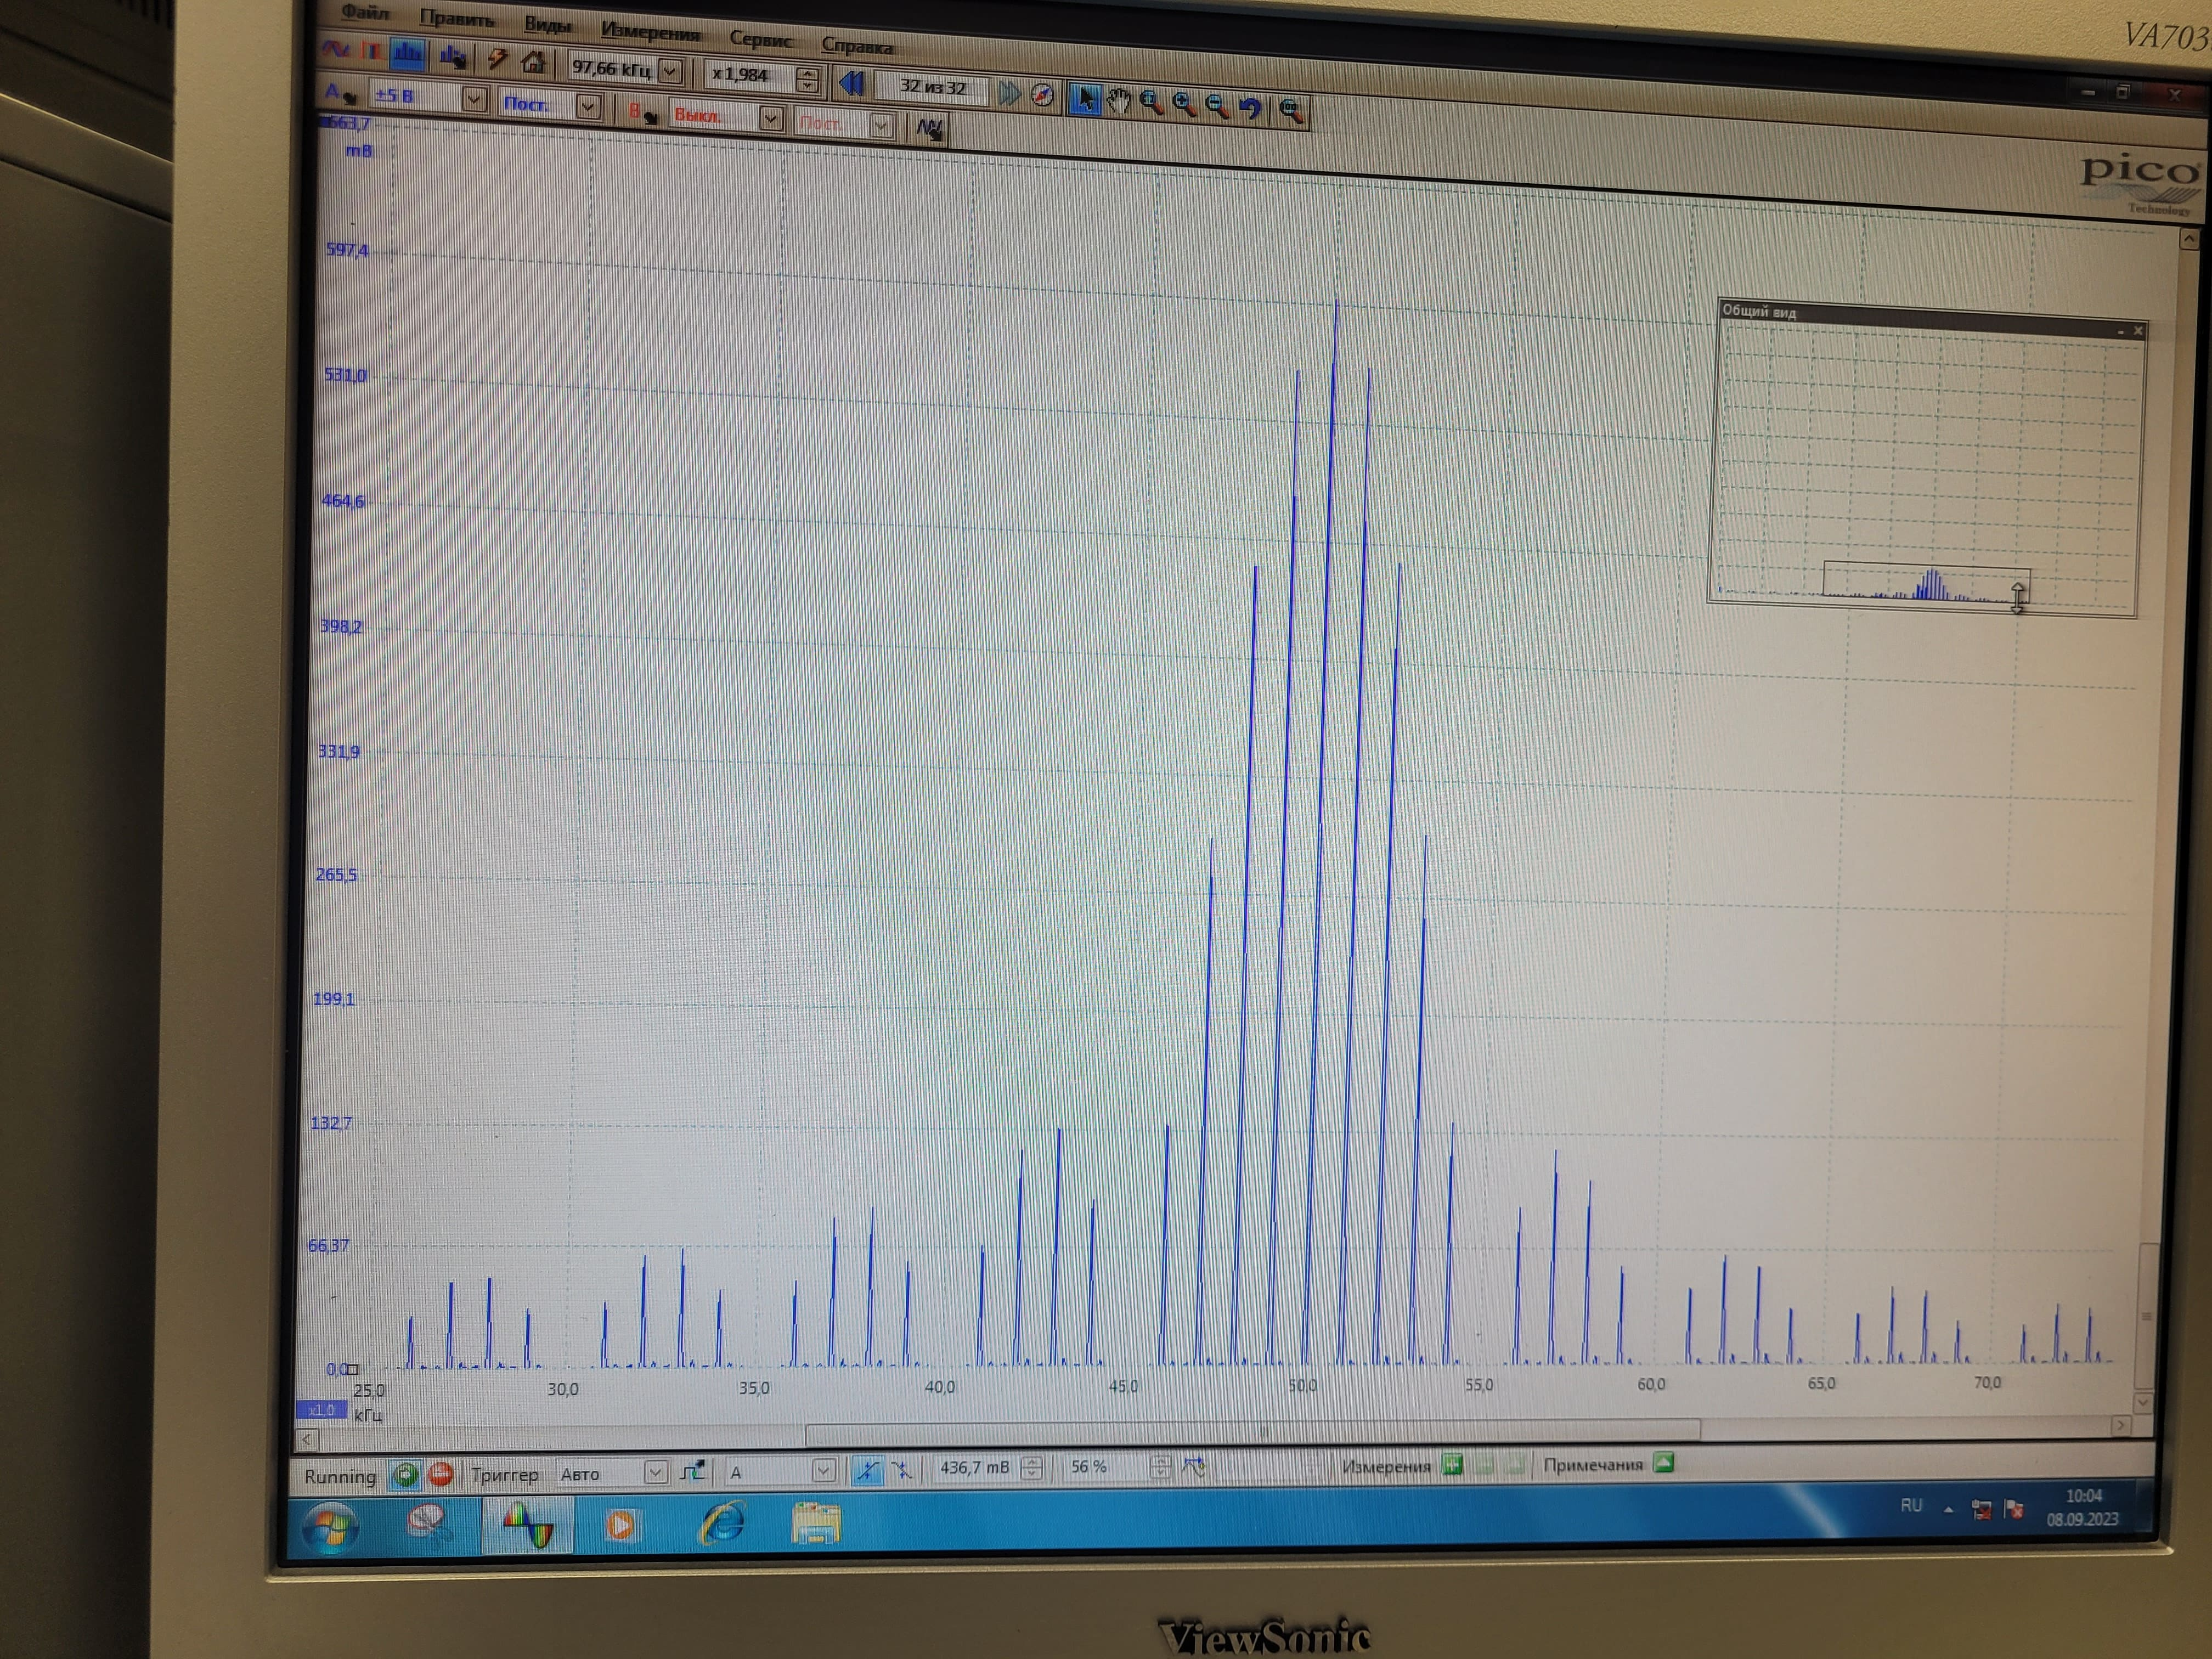
\includegraphics[width=1\linewidth]{B_50k_1k_10.jpg}} \\N=10, $\delta \nu$ = 1 кГц, $\Delta \nu$ = 5 кГц
\end{minipage}
\vfill
\begin{minipage}[h]{0.47\linewidth}
\center{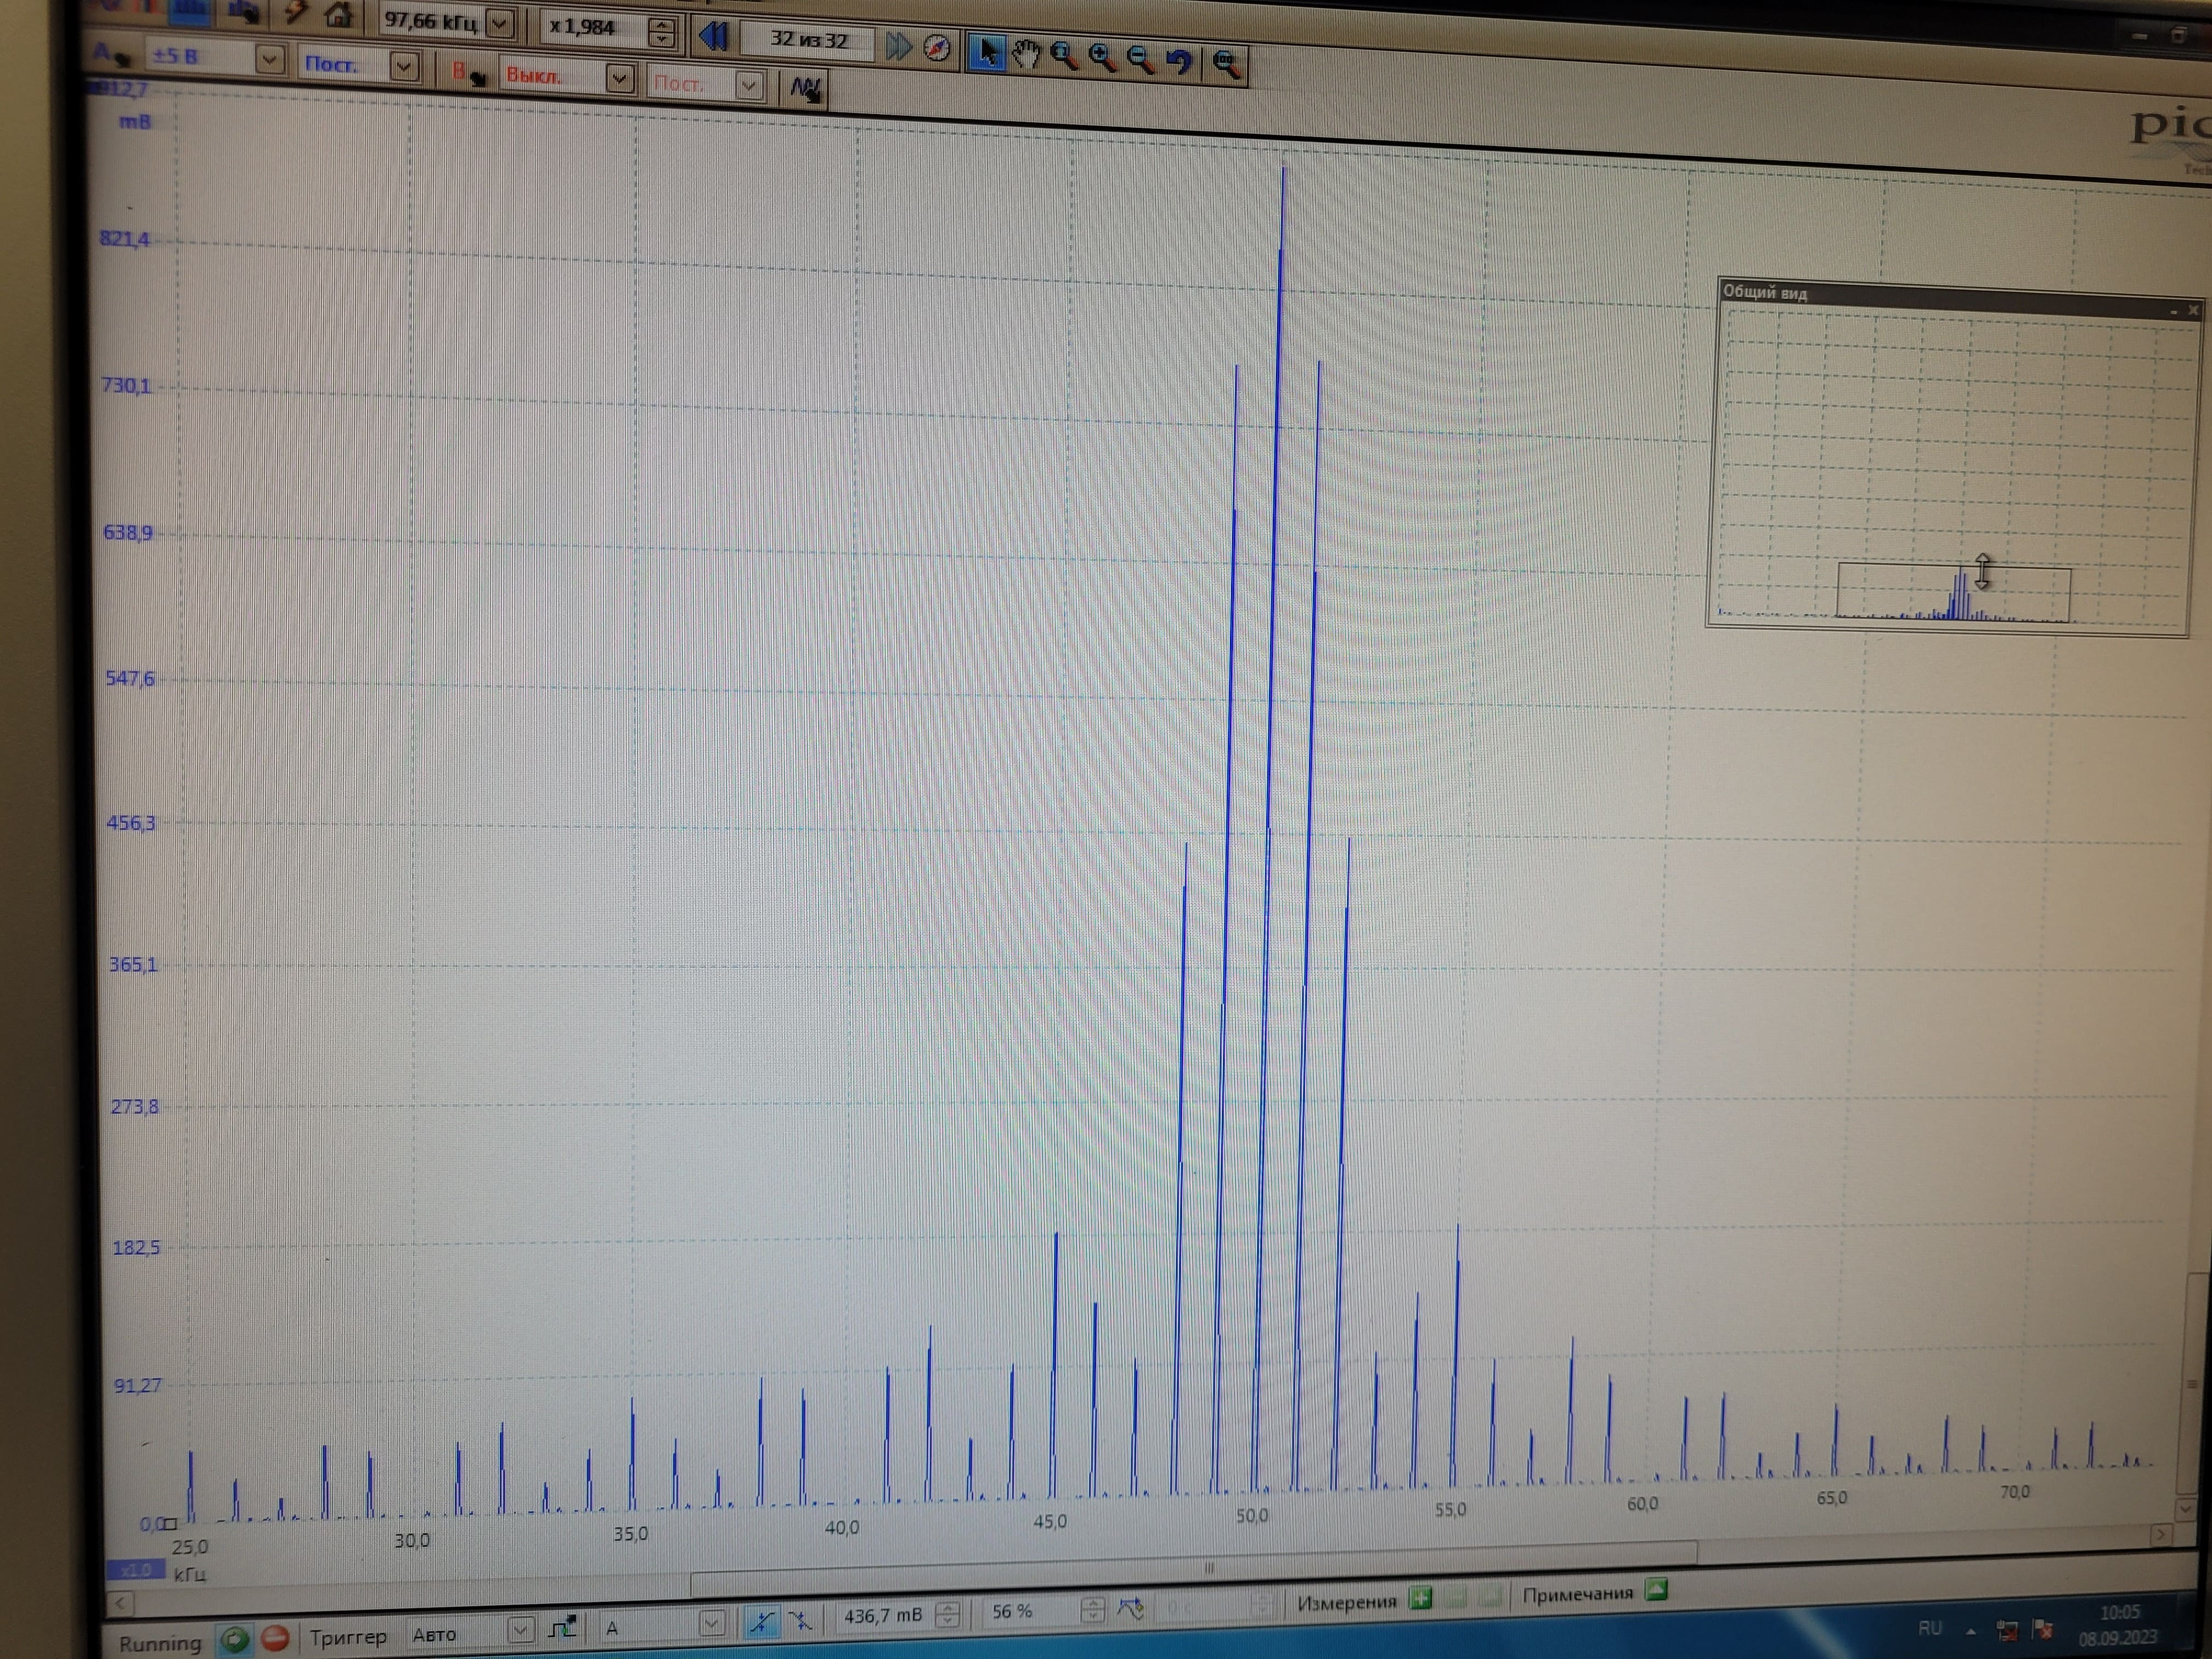
\includegraphics[width=1\linewidth]{B_50k_1k_15.jpg}} N=15, $\delta \nu$ = 1 кГц, $\Delta \nu$ $\approx$ 3 кГц \\
\end{minipage}
\hfill
\begin{minipage}[h]{0.47\linewidth}
\center{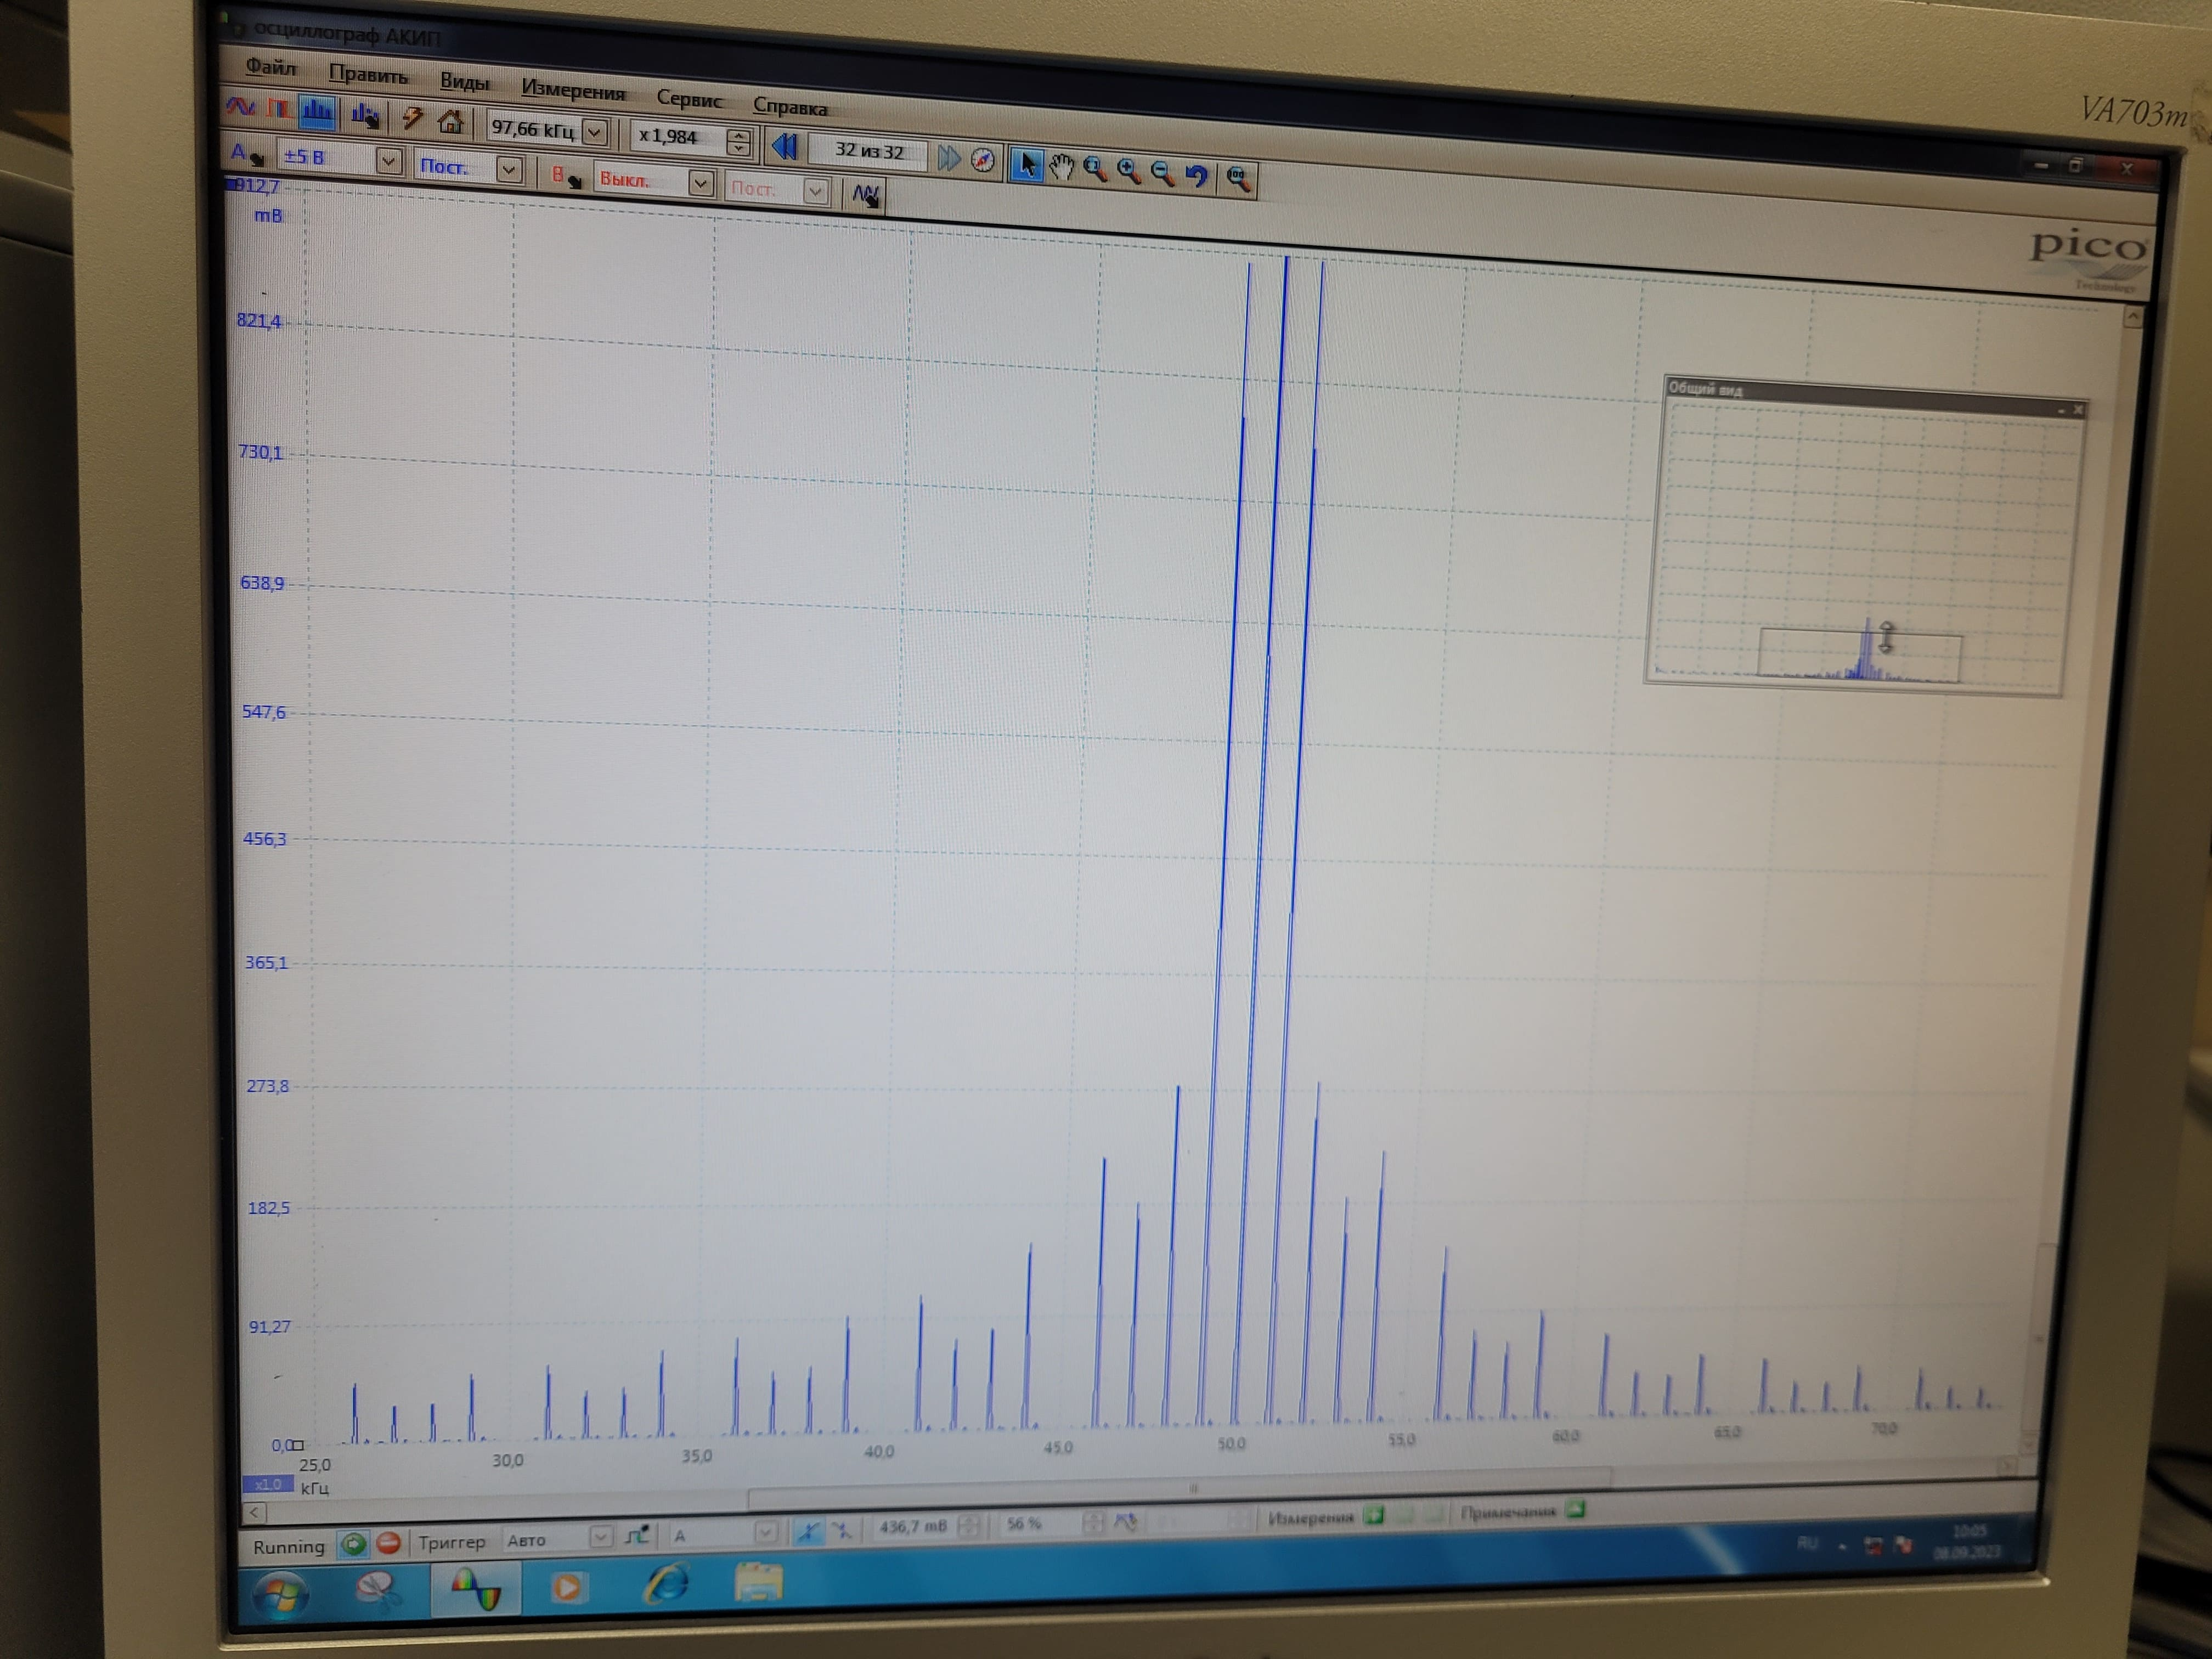
\includegraphics[width=1\linewidth]{B_50k_1k_20.jpg}} N=20, $\delta \nu$ = 1 кГц, $\Delta \nu$ $\approx$ 2.5 кГц \\
\end{minipage}
\caption{}
\label{ris:experimentalcorrelationsignals}
\end{figure}

Соотношение неопределённостей:
$$ \Delta \nu \cdot \tau = 10\cdot10^3\frac{5}{50\cdot10^3} = 5\cdot10^3\frac{10}{50\cdot10^3} = 2.5\cdot10^3\frac{20}{50\cdot10^3} \approx 3\cdot10^3\frac{15}{50\cdot10^3} \approx 1 $$\\

Видим, что спектр остаётся симметричным относительно одной и той же точки, однако "сжимается" к ней при увеличении N.


\newpage

\textbf{б.} Изменяем $\nu_0$ при фиксированных N = 5 и $\nu_\text{повт}$ = 1 кГц:

\begin{figure}[h]
\begin{minipage}[h]{0.47\linewidth}
\center{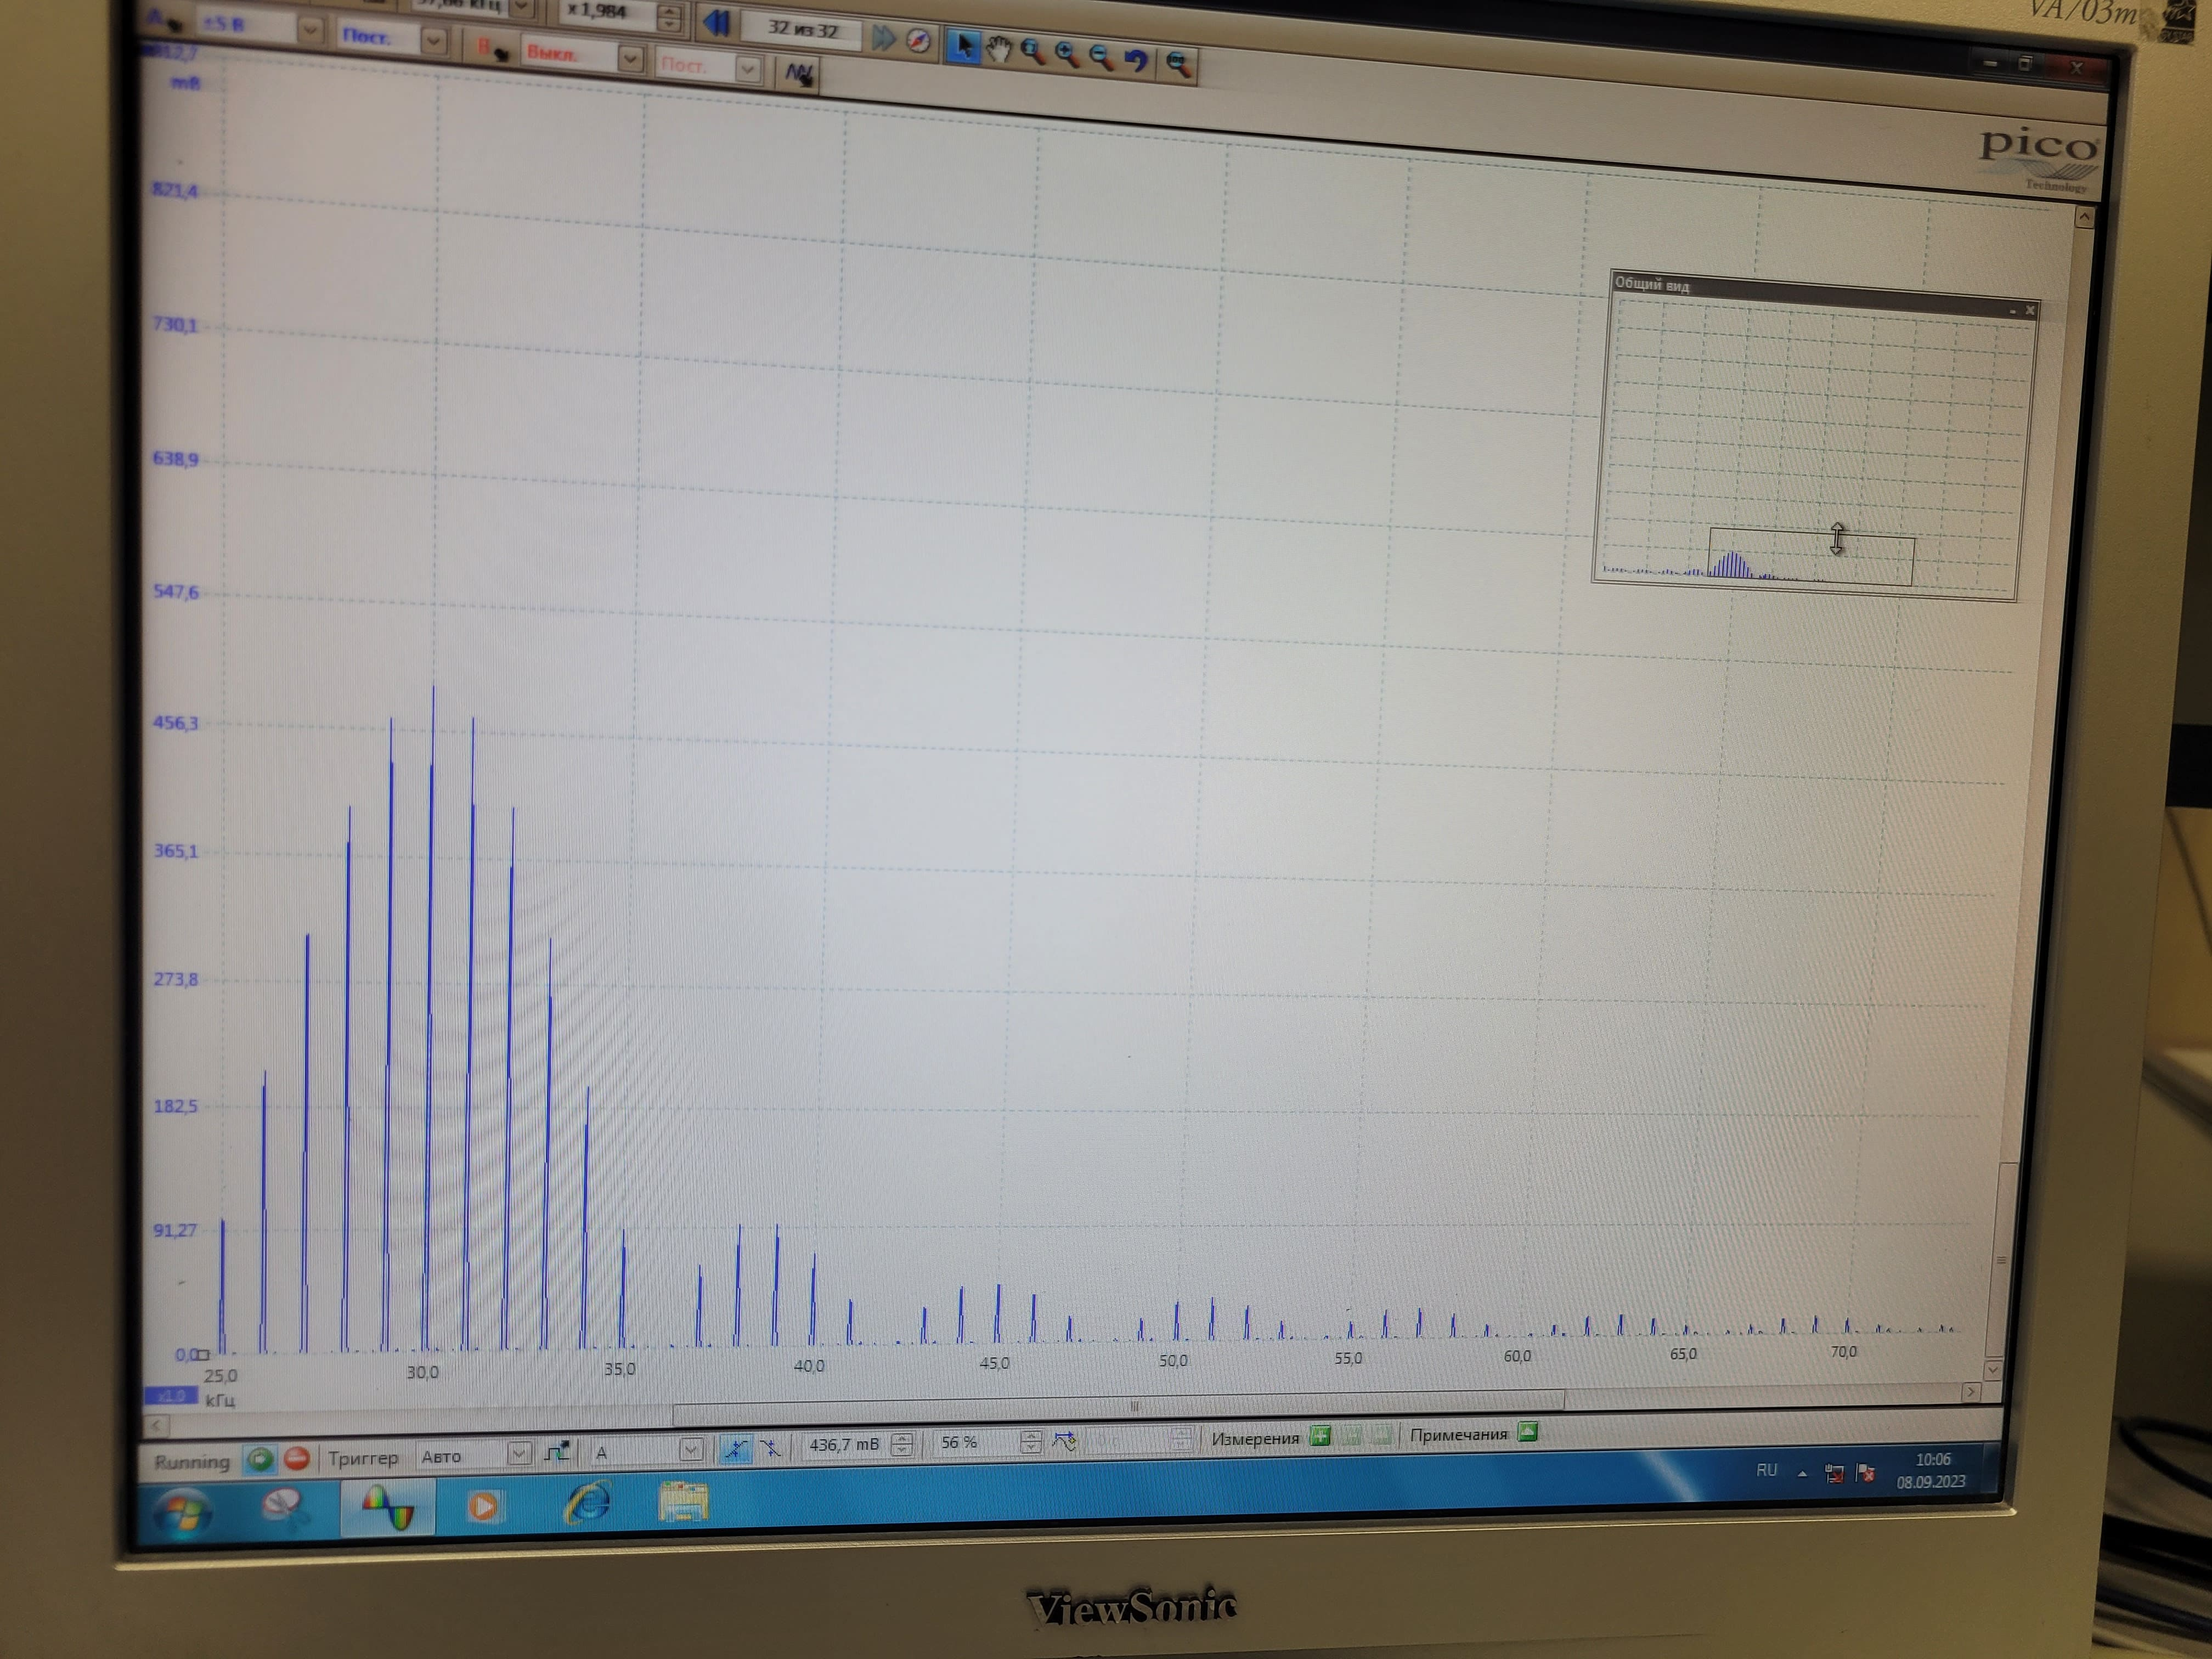
\includegraphics[width=1\linewidth]{B_30k_1k_5.jpg}} $\nu_0$ = 30 кГц, $\delta \nu$ = 1 кГц, $\Delta \nu$ = 6 кГц  \\
\end{minipage}
\hfill
\begin{minipage}[h]{0.47\linewidth}
\center{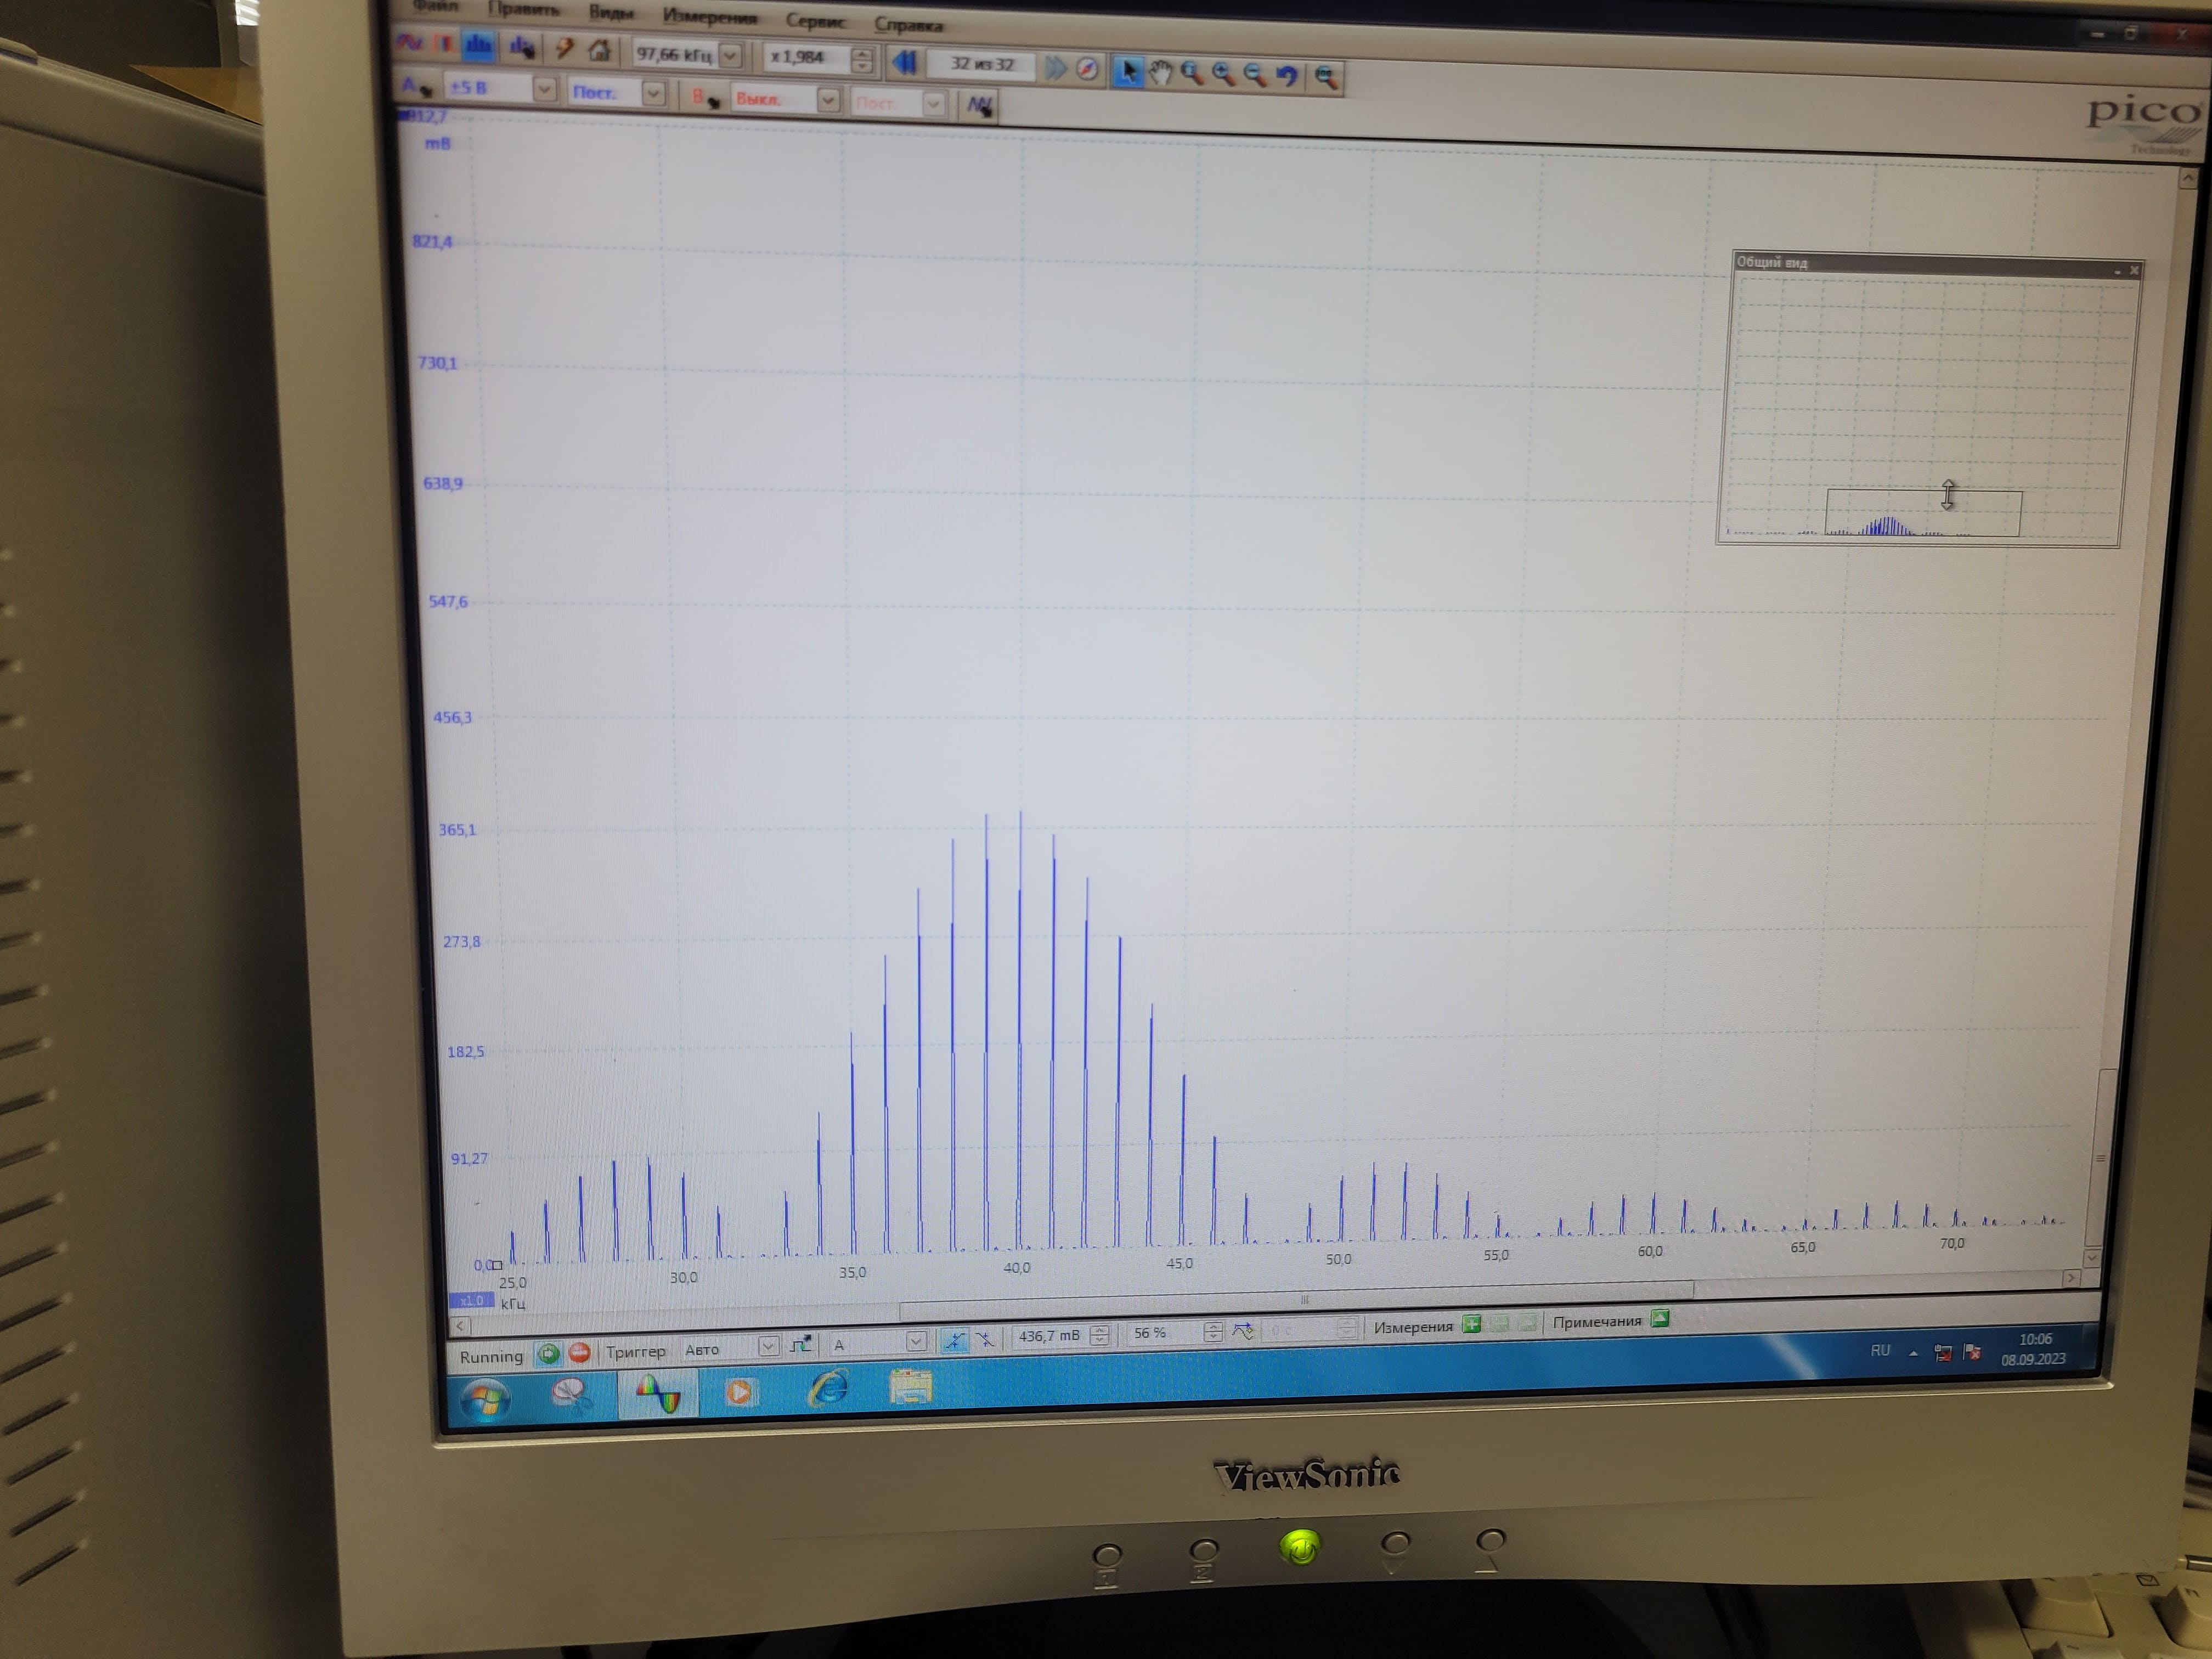
\includegraphics[width=1\linewidth]{B_40k_1k_5.jpg}} \\ $\nu_0$ = 40 кГц, $\delta \nu$ = 1 кГц, $\Delta \nu$ = 8 кГц
\end{minipage}
\vfill
\begin{minipage}[h]{0.47\linewidth}
\center{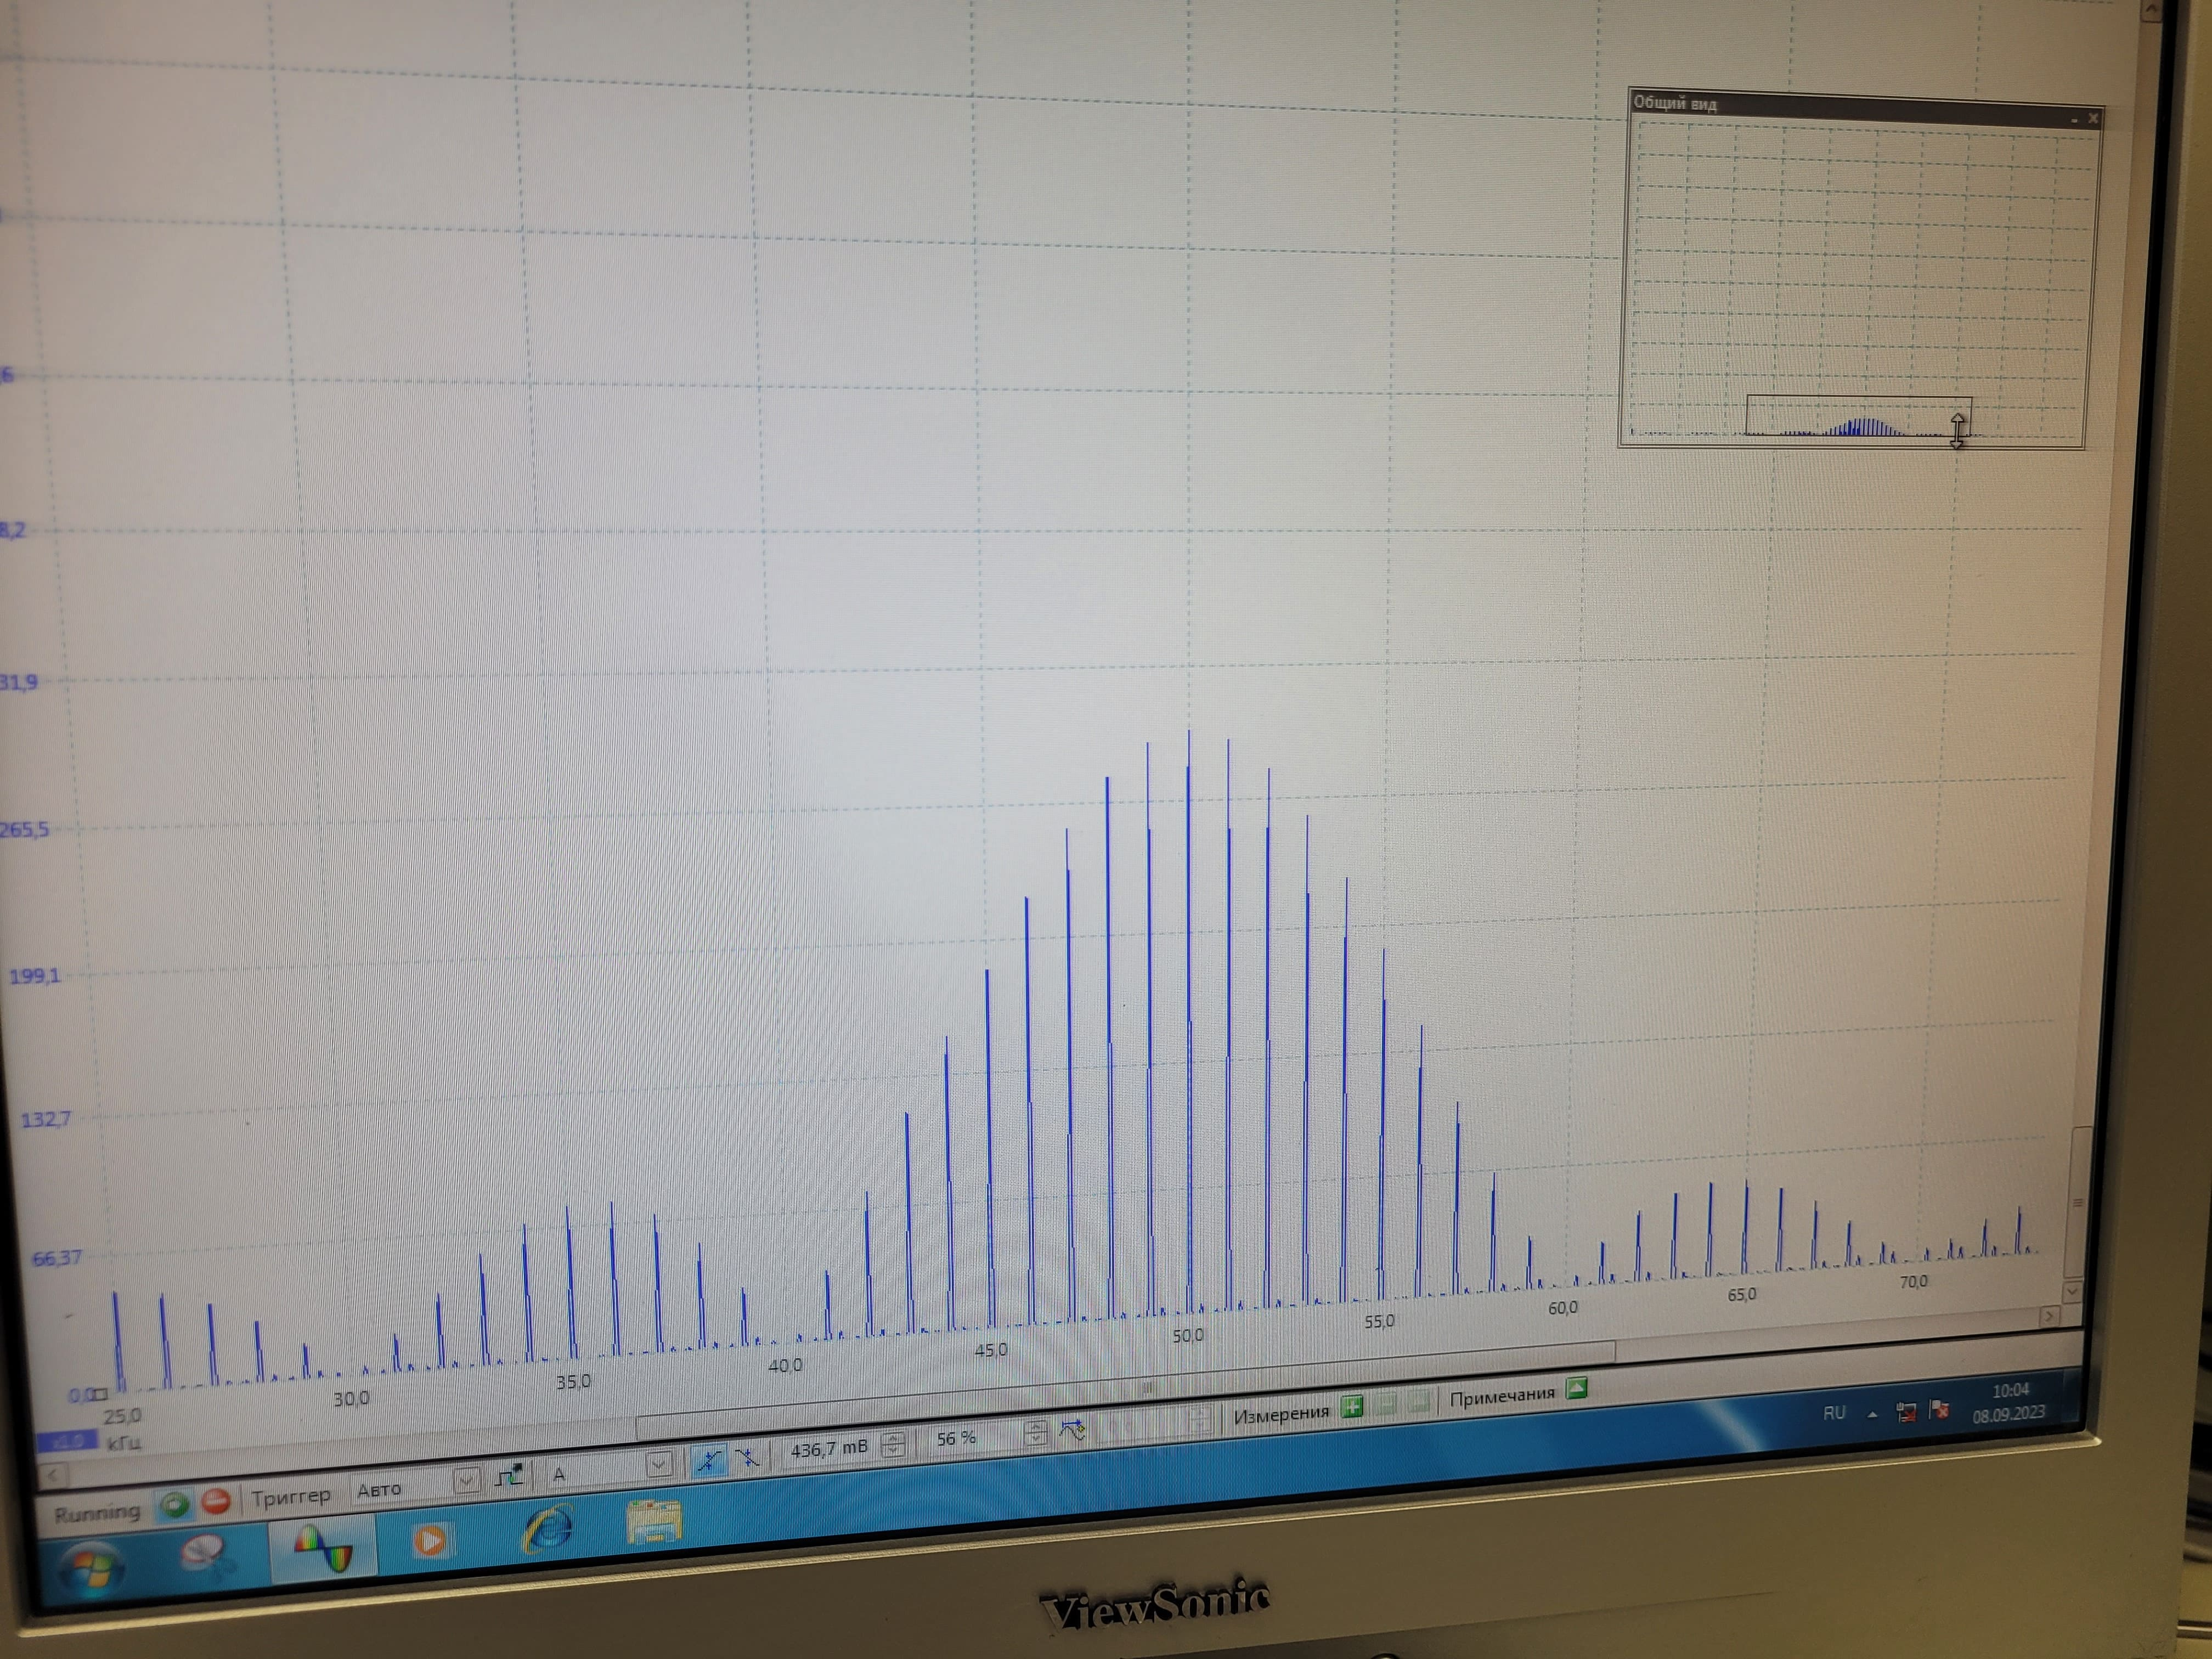
\includegraphics[width=1\linewidth]{B_50k_1k_5.jpg}} $\nu_0$ = 50 кГц, $\delta \nu$ = 1 кГц, $\Delta \nu$ = 10 кГц \\
\end{minipage}
\hfill
\caption{}
\label{ris:experimentalcorrelationsignals}
\end{figure}

Соотношение неопределённостей:
$$ \Delta \nu \cdot \tau = 6\cdot10^3\frac{5}{30\cdot10^3} = 8\cdot10^3\frac{5}{40\cdot10^3} = 10\cdot10^3\frac{5}{50\cdot10^3} = 1 $$\\
Видим, что в этом случае спектр не меняет свою форму, однако его центр смещается в соответсвии с изменением частоты несущей.


\newpage

\textbf{в.} Изменяем $\nu_\text{повт}$  при фиксированных N = 5 и $\nu_0$ = 50 кГц:

\begin{figure}[h]
\begin{minipage}[h]{0.47\linewidth}
\center{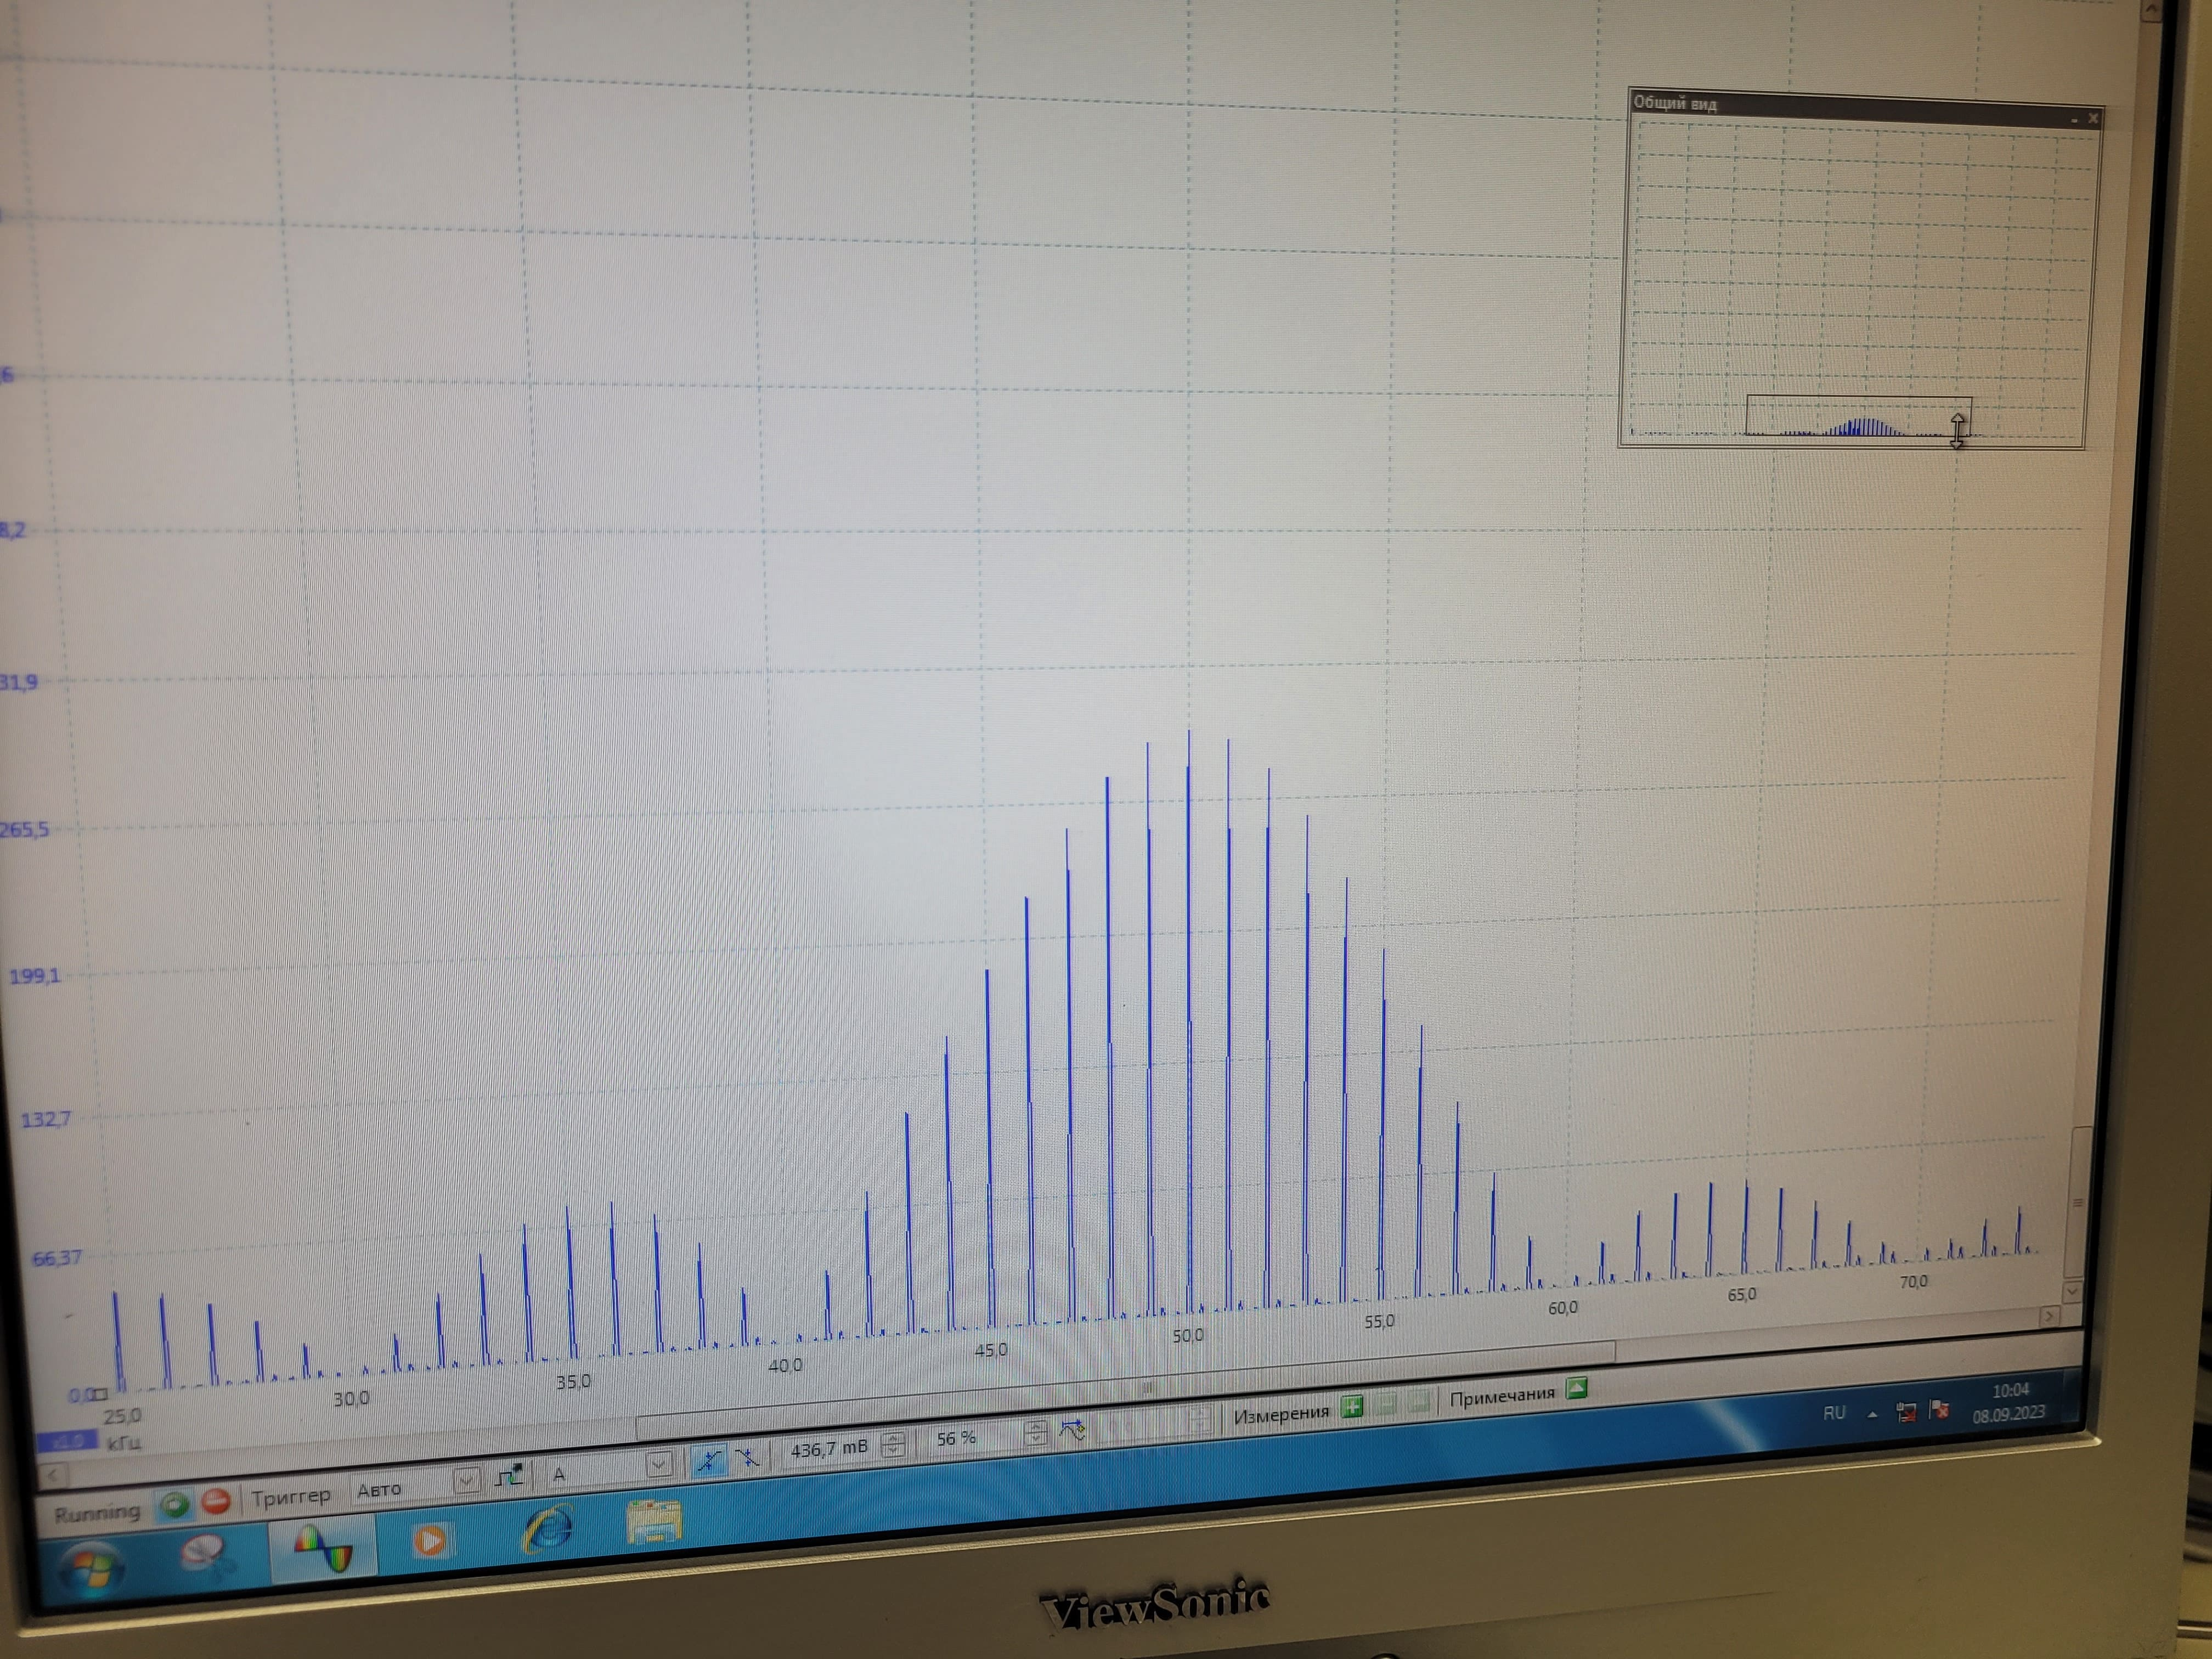
\includegraphics[width=1\linewidth]{B_50k_1k_5.jpg}} $\nu_\text{повт}$  = 1 кГц, $\delta \nu$ = 1 кГц, $\Delta \nu$ = 10 кГц \\
\end{minipage}
\hfill
\begin{minipage}[h]{0.47\linewidth}
\center{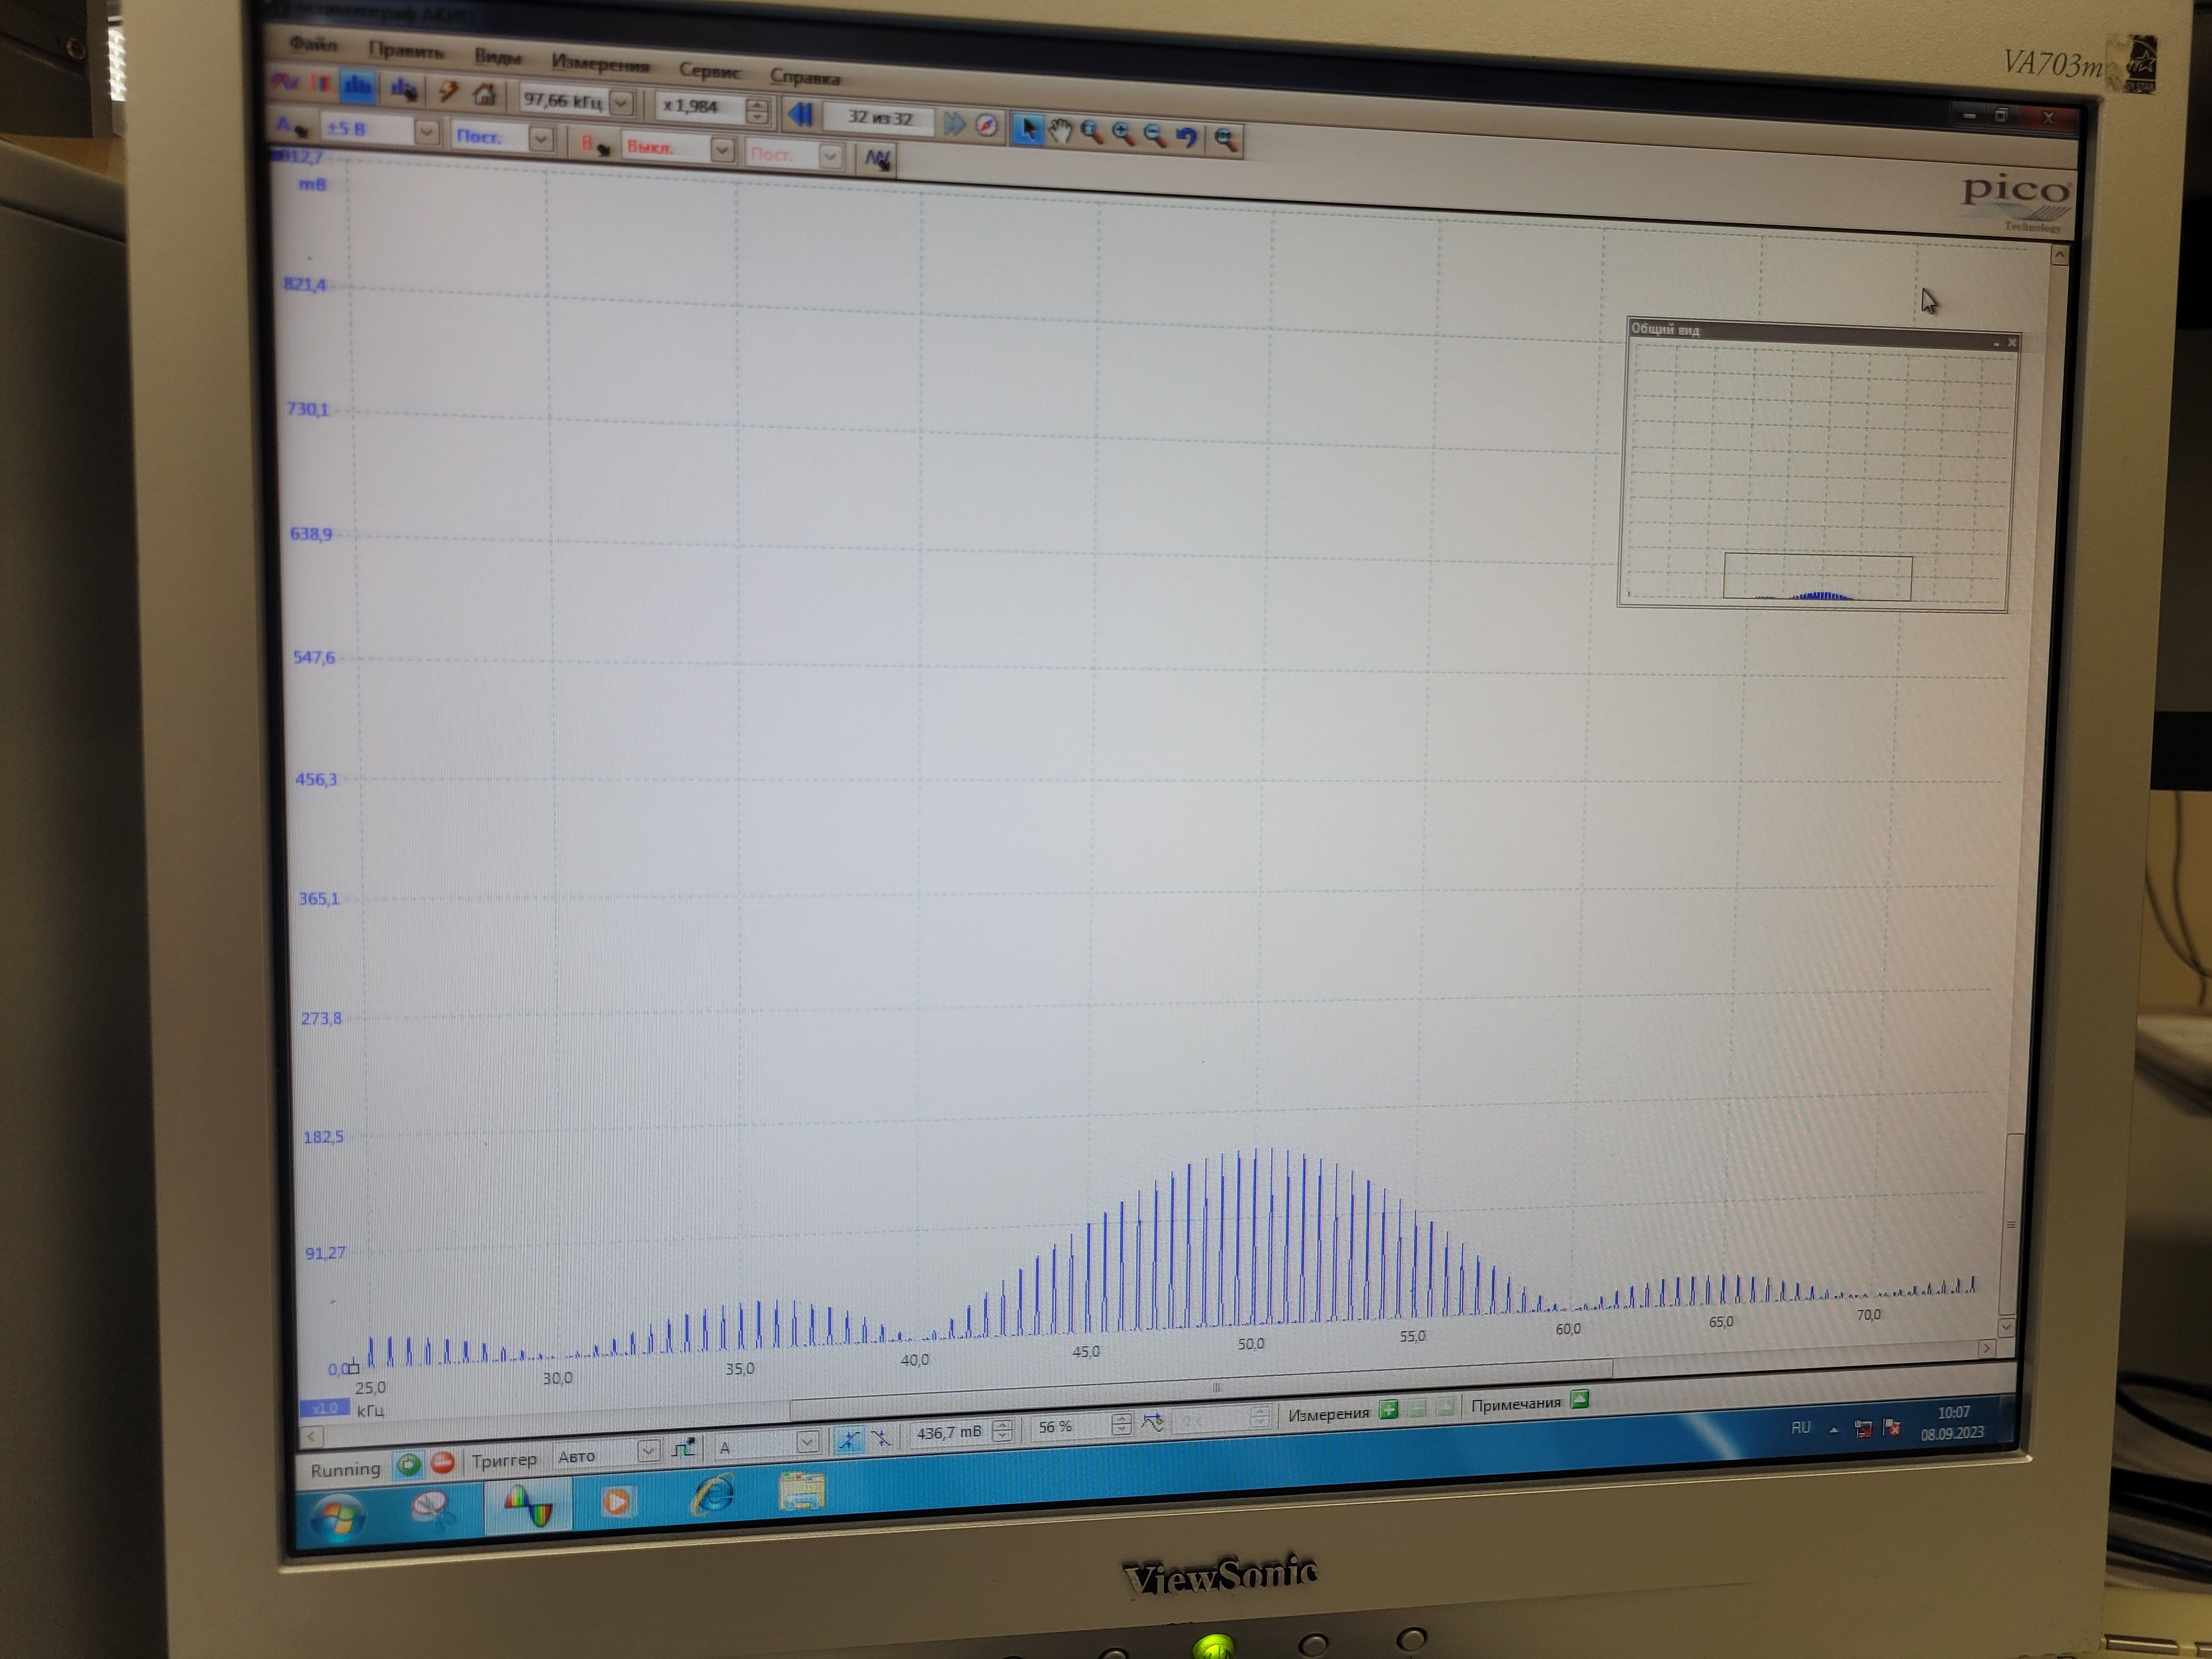
\includegraphics[width=1\linewidth]{B_50k_2k_5.jpg}} \\ $\nu_\text{повт}$  = 0.5 кГц, $\delta \nu$ = 0.5 кГц, $\Delta \nu$ = 10 кГц
\end{minipage}
\vfill
\begin{minipage}[h]{0.47\linewidth}
\center{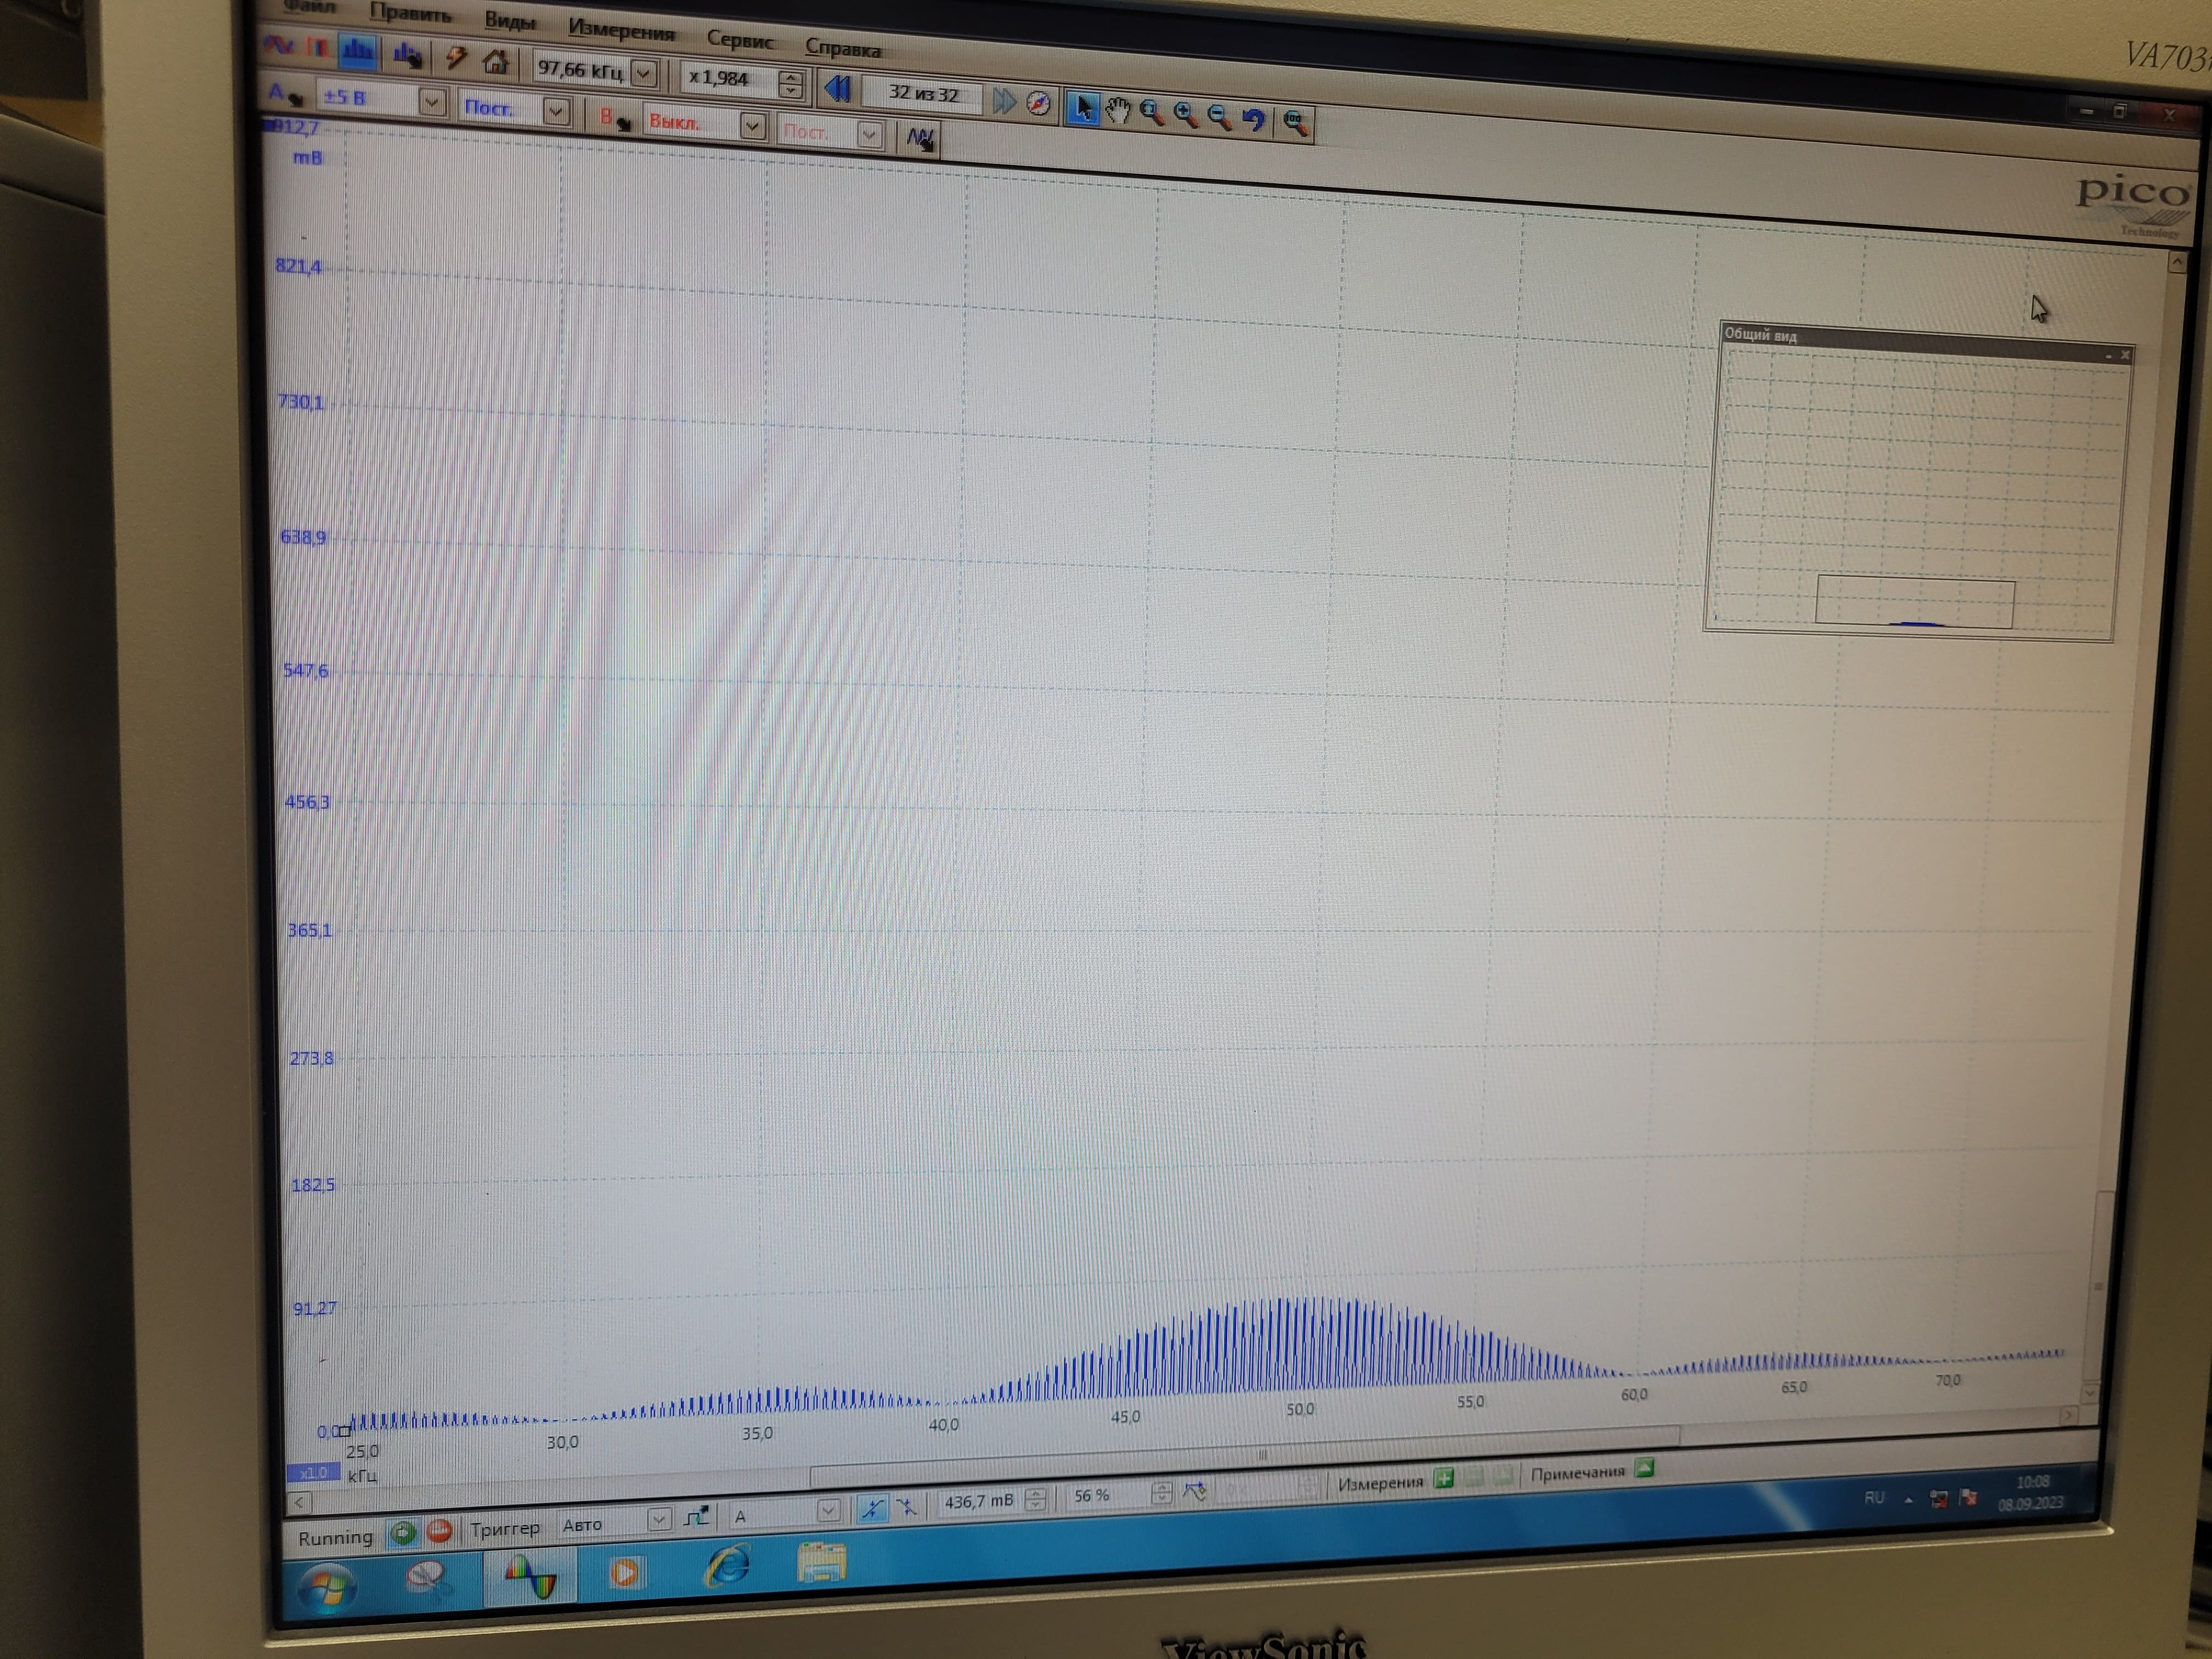
\includegraphics[width=1\linewidth]{B_50k_4k_5.jpg}} $\nu_\text{повт}$  = 0.25 кГц, $\delta \nu$ = 0.25 кГц, $\Delta \nu$ = 10 кГц \\
\end{minipage}
\hfill
\caption{}
\label{ris:experimentalcorrelationsignals}
\end{figure}

Видно, что соотношение неопределённости выполняется:
$$ \frac{\delta \nu}{\nu_\text{повт}} = \frac{1\cdot10^3}{1\cdot10^3} = \frac{0.5\cdot10^3}{0.5\cdot10^3} = \frac{0.25\cdot10^3}{0.25\cdot10^3} = 1 $$\\

Также видно, что при стремлении частоты повторения к нулю, стремится к нулю и расстояние между компонентами спектра.

\end{enumerate}


















\newpage

% \subsection*{В. Наблюдение спектра периодической последовательности гауссианов}
% \begin{figure}[h]
%     \centering
%     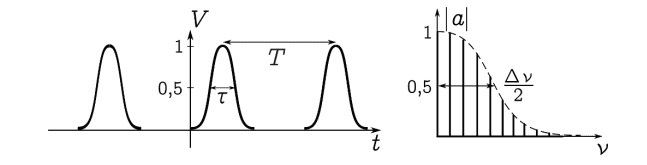
\includegraphics[width=0.7\linewidth]{gausiana.png}
%     \caption{Периодическая последовательность гауссианов и ее спектр}
%     \label{gausiana}
% \end{figure}

% \begin{enumerate}


% \item [\textbf{1.}] Настраиваем генератор в режим передачи периодической последовательности \textit{"гауссианов"} с несущей частотой $\nu_0$ = 50 кГц и периодом повторения $T$ = 10 мс.

% \item [\textbf{2.}] Получаем на экране спектр (Преобразование Фурье) сигнала.

% \textbf{a.} Изменяем $\nu_0$ при фиксированных $T$ = 10 мс.


% \begin{figure}[h]
% \begin{minipage}[h]{0.47\linewidth}
% \center{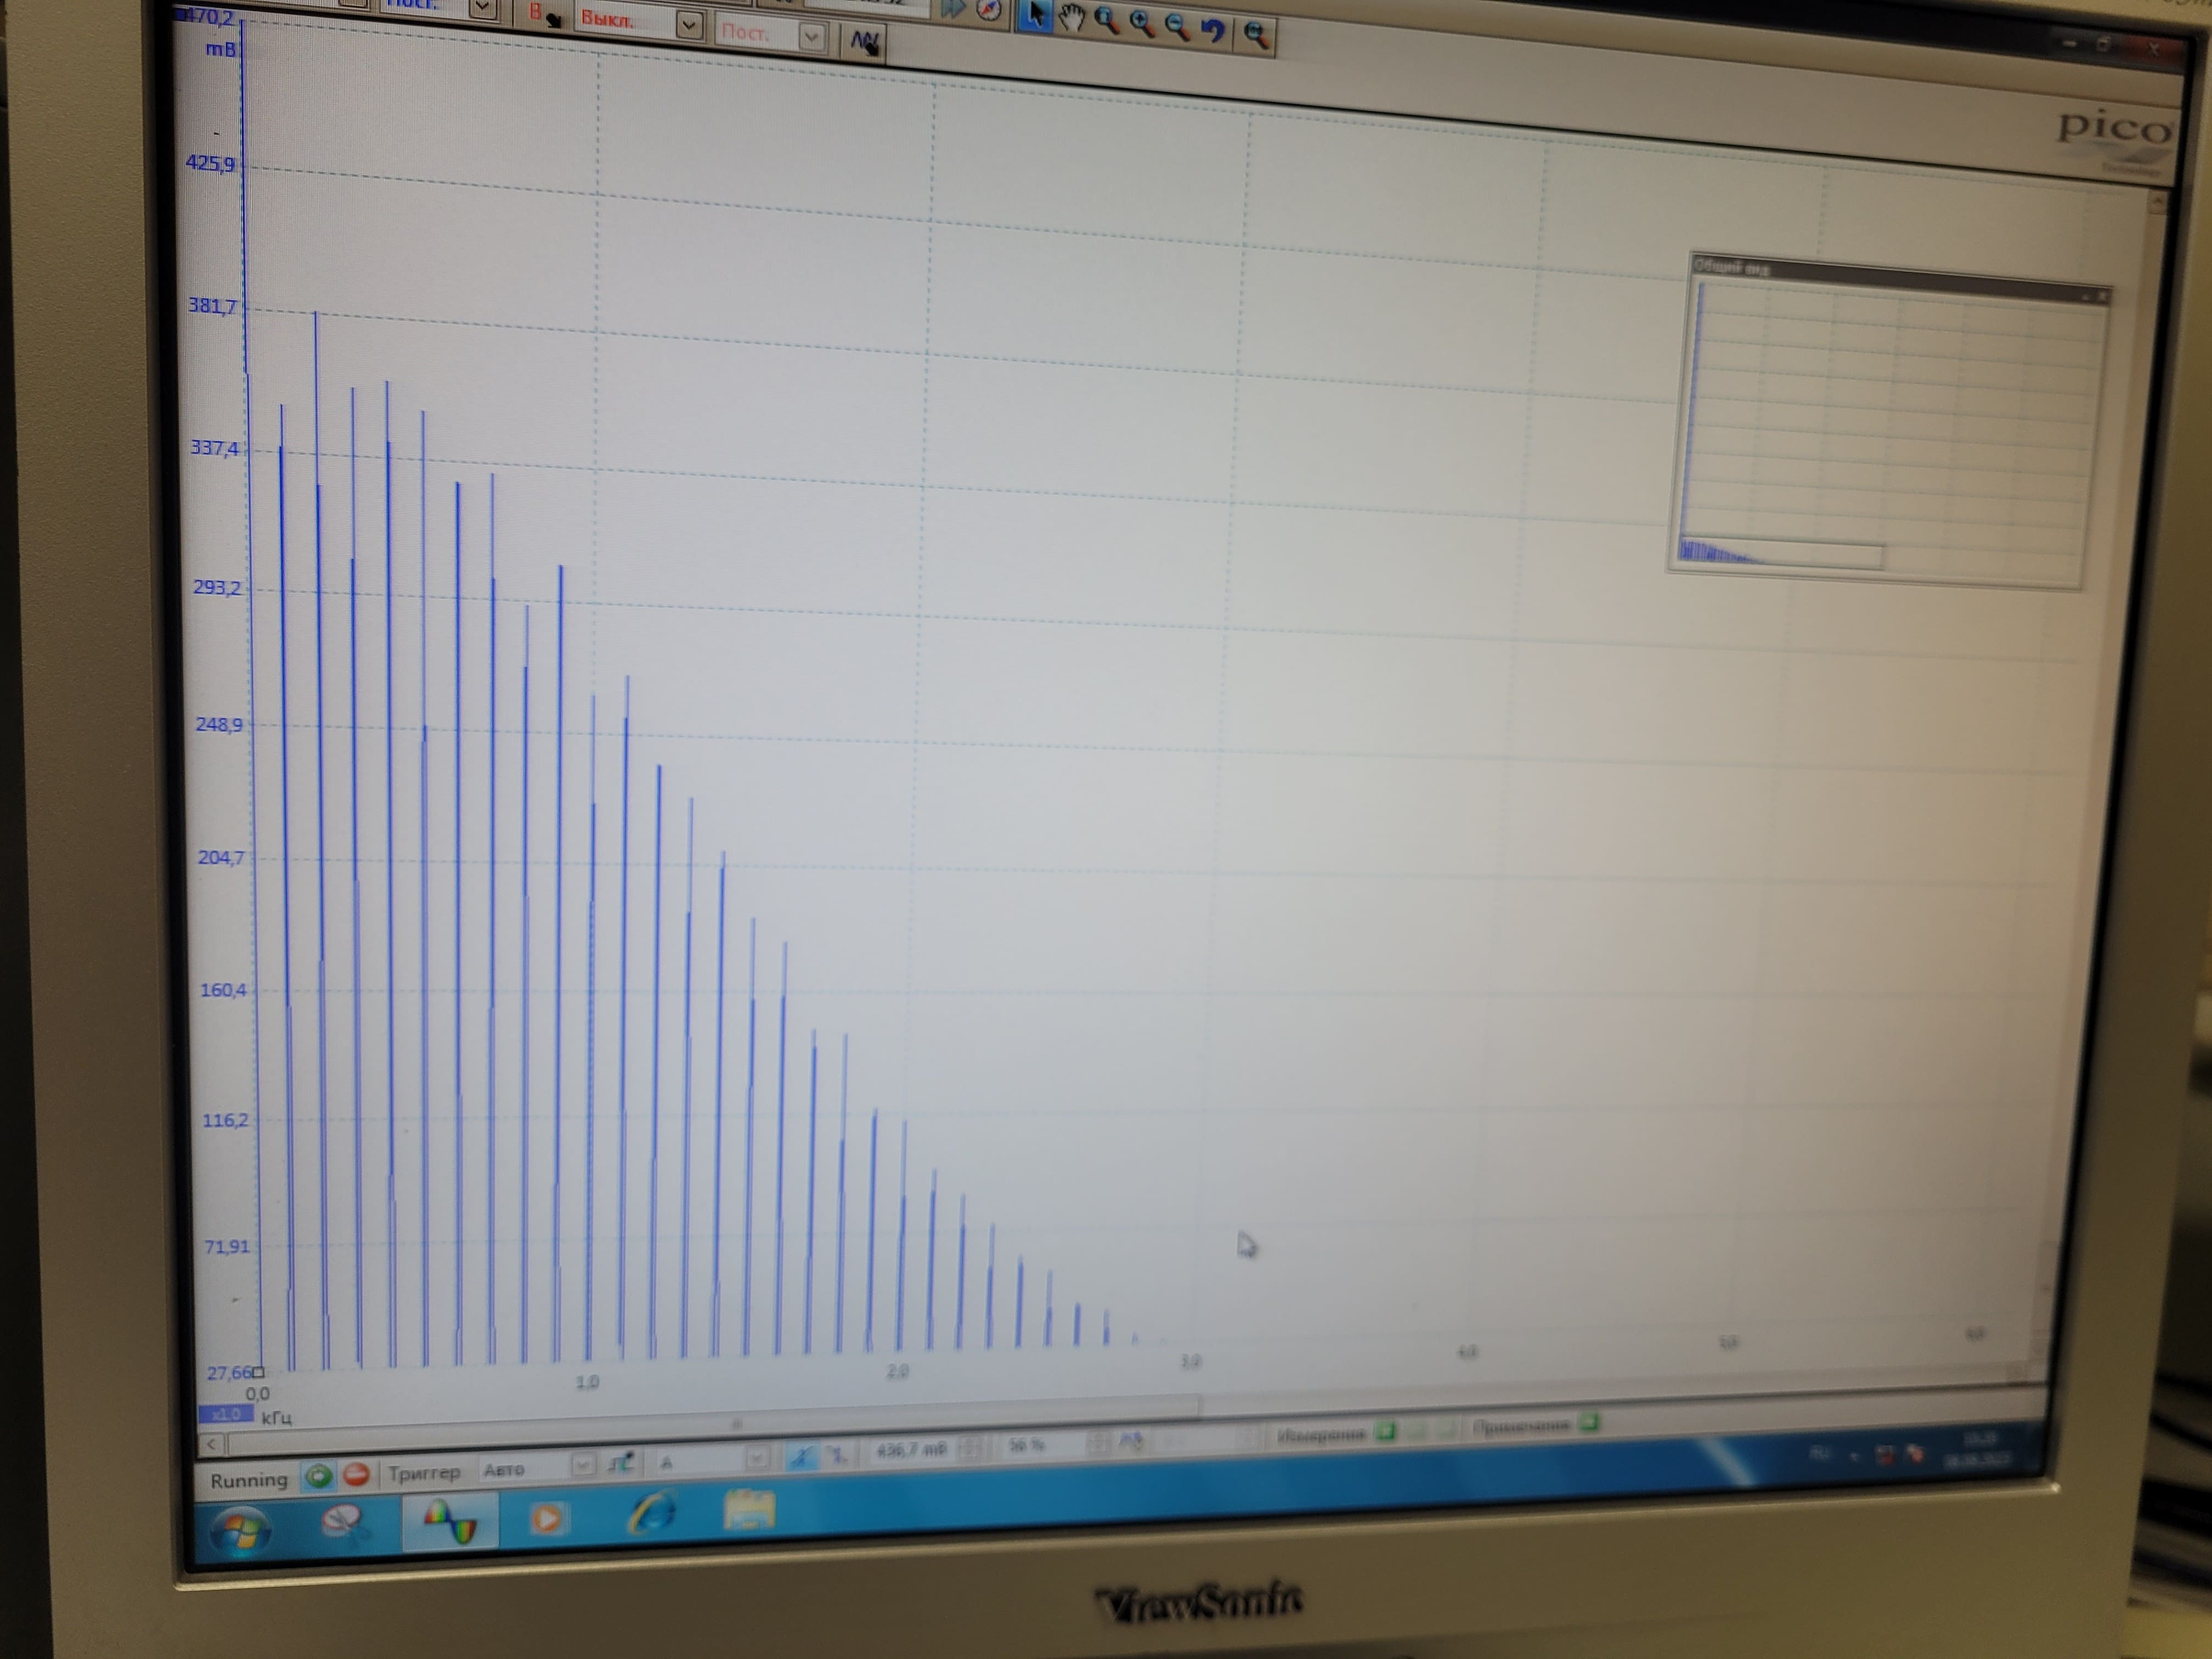
\includegraphics[width=1\linewidth]{V_1k_10T.jpg}} $\nu$ = 1 кГц \\
% \end{minipage}
% \hfill
% \begin{minipage}[h]{0.47\linewidth}
% \center{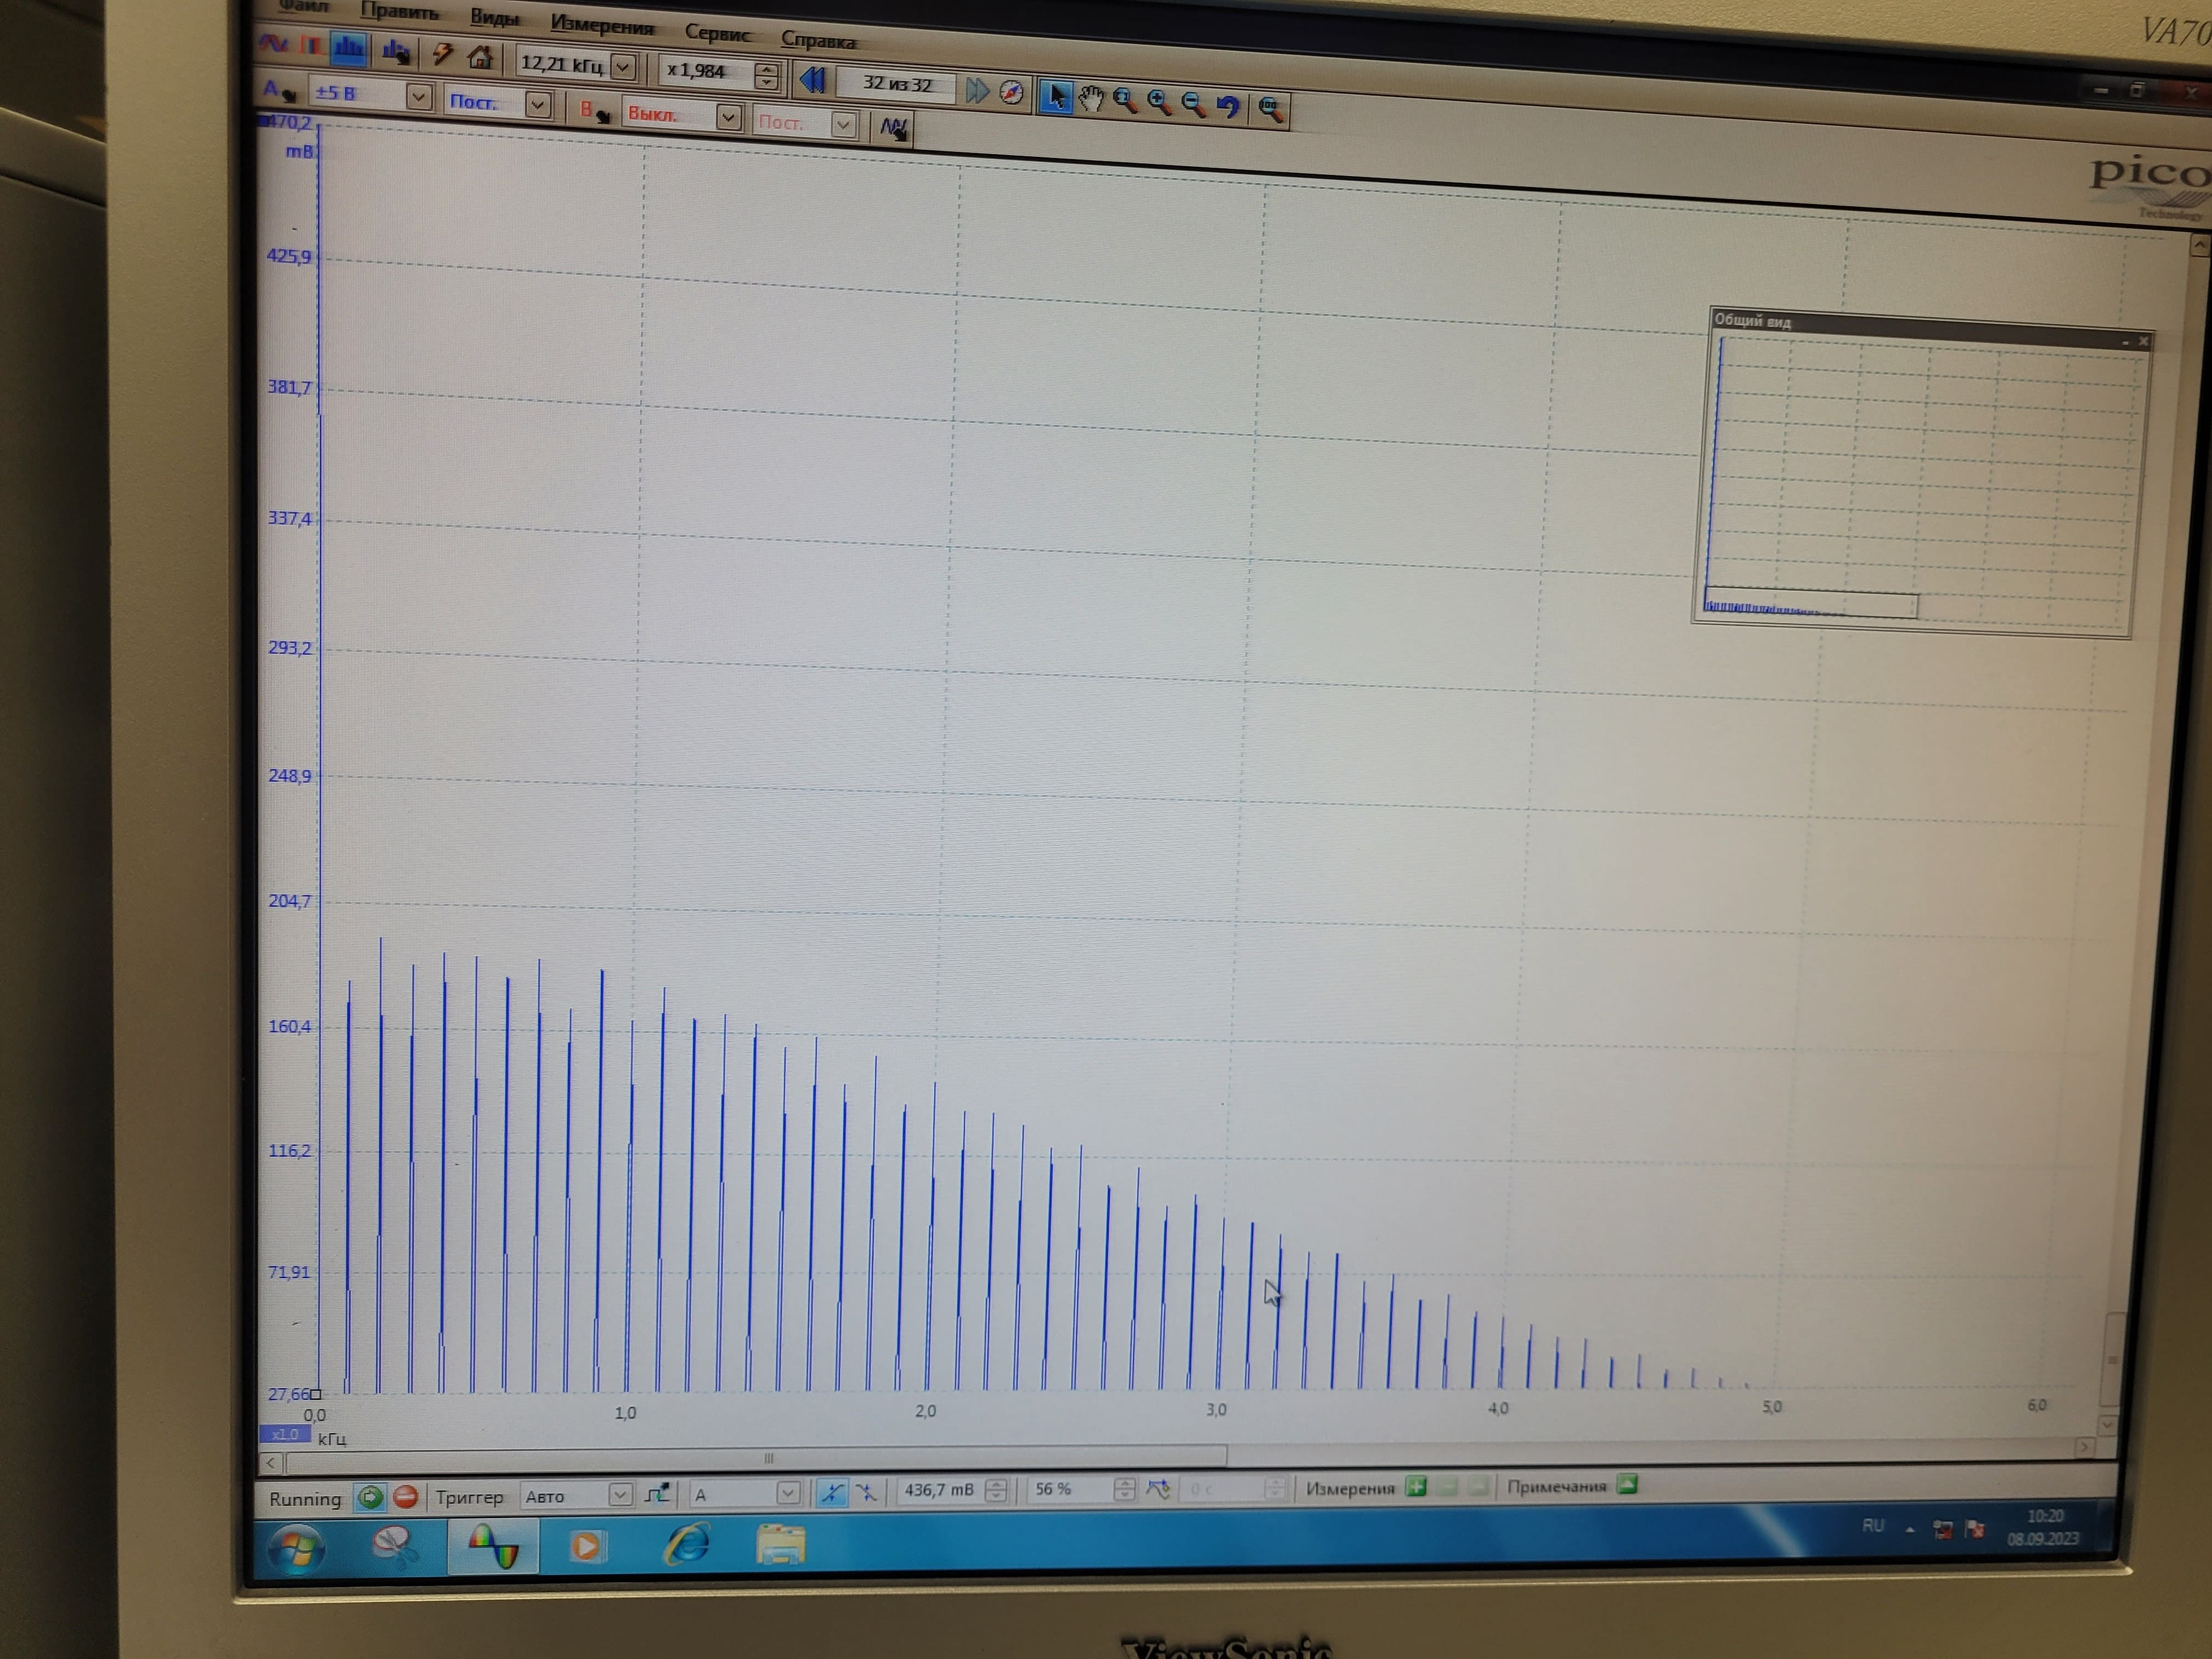
\includegraphics[width=1\linewidth]{V_2k_10T.jpg}} \\$\nu$ = 2 кГц
% \end{minipage}
% \vfill
% \begin{minipage}[h]{0.47\linewidth}
% \center{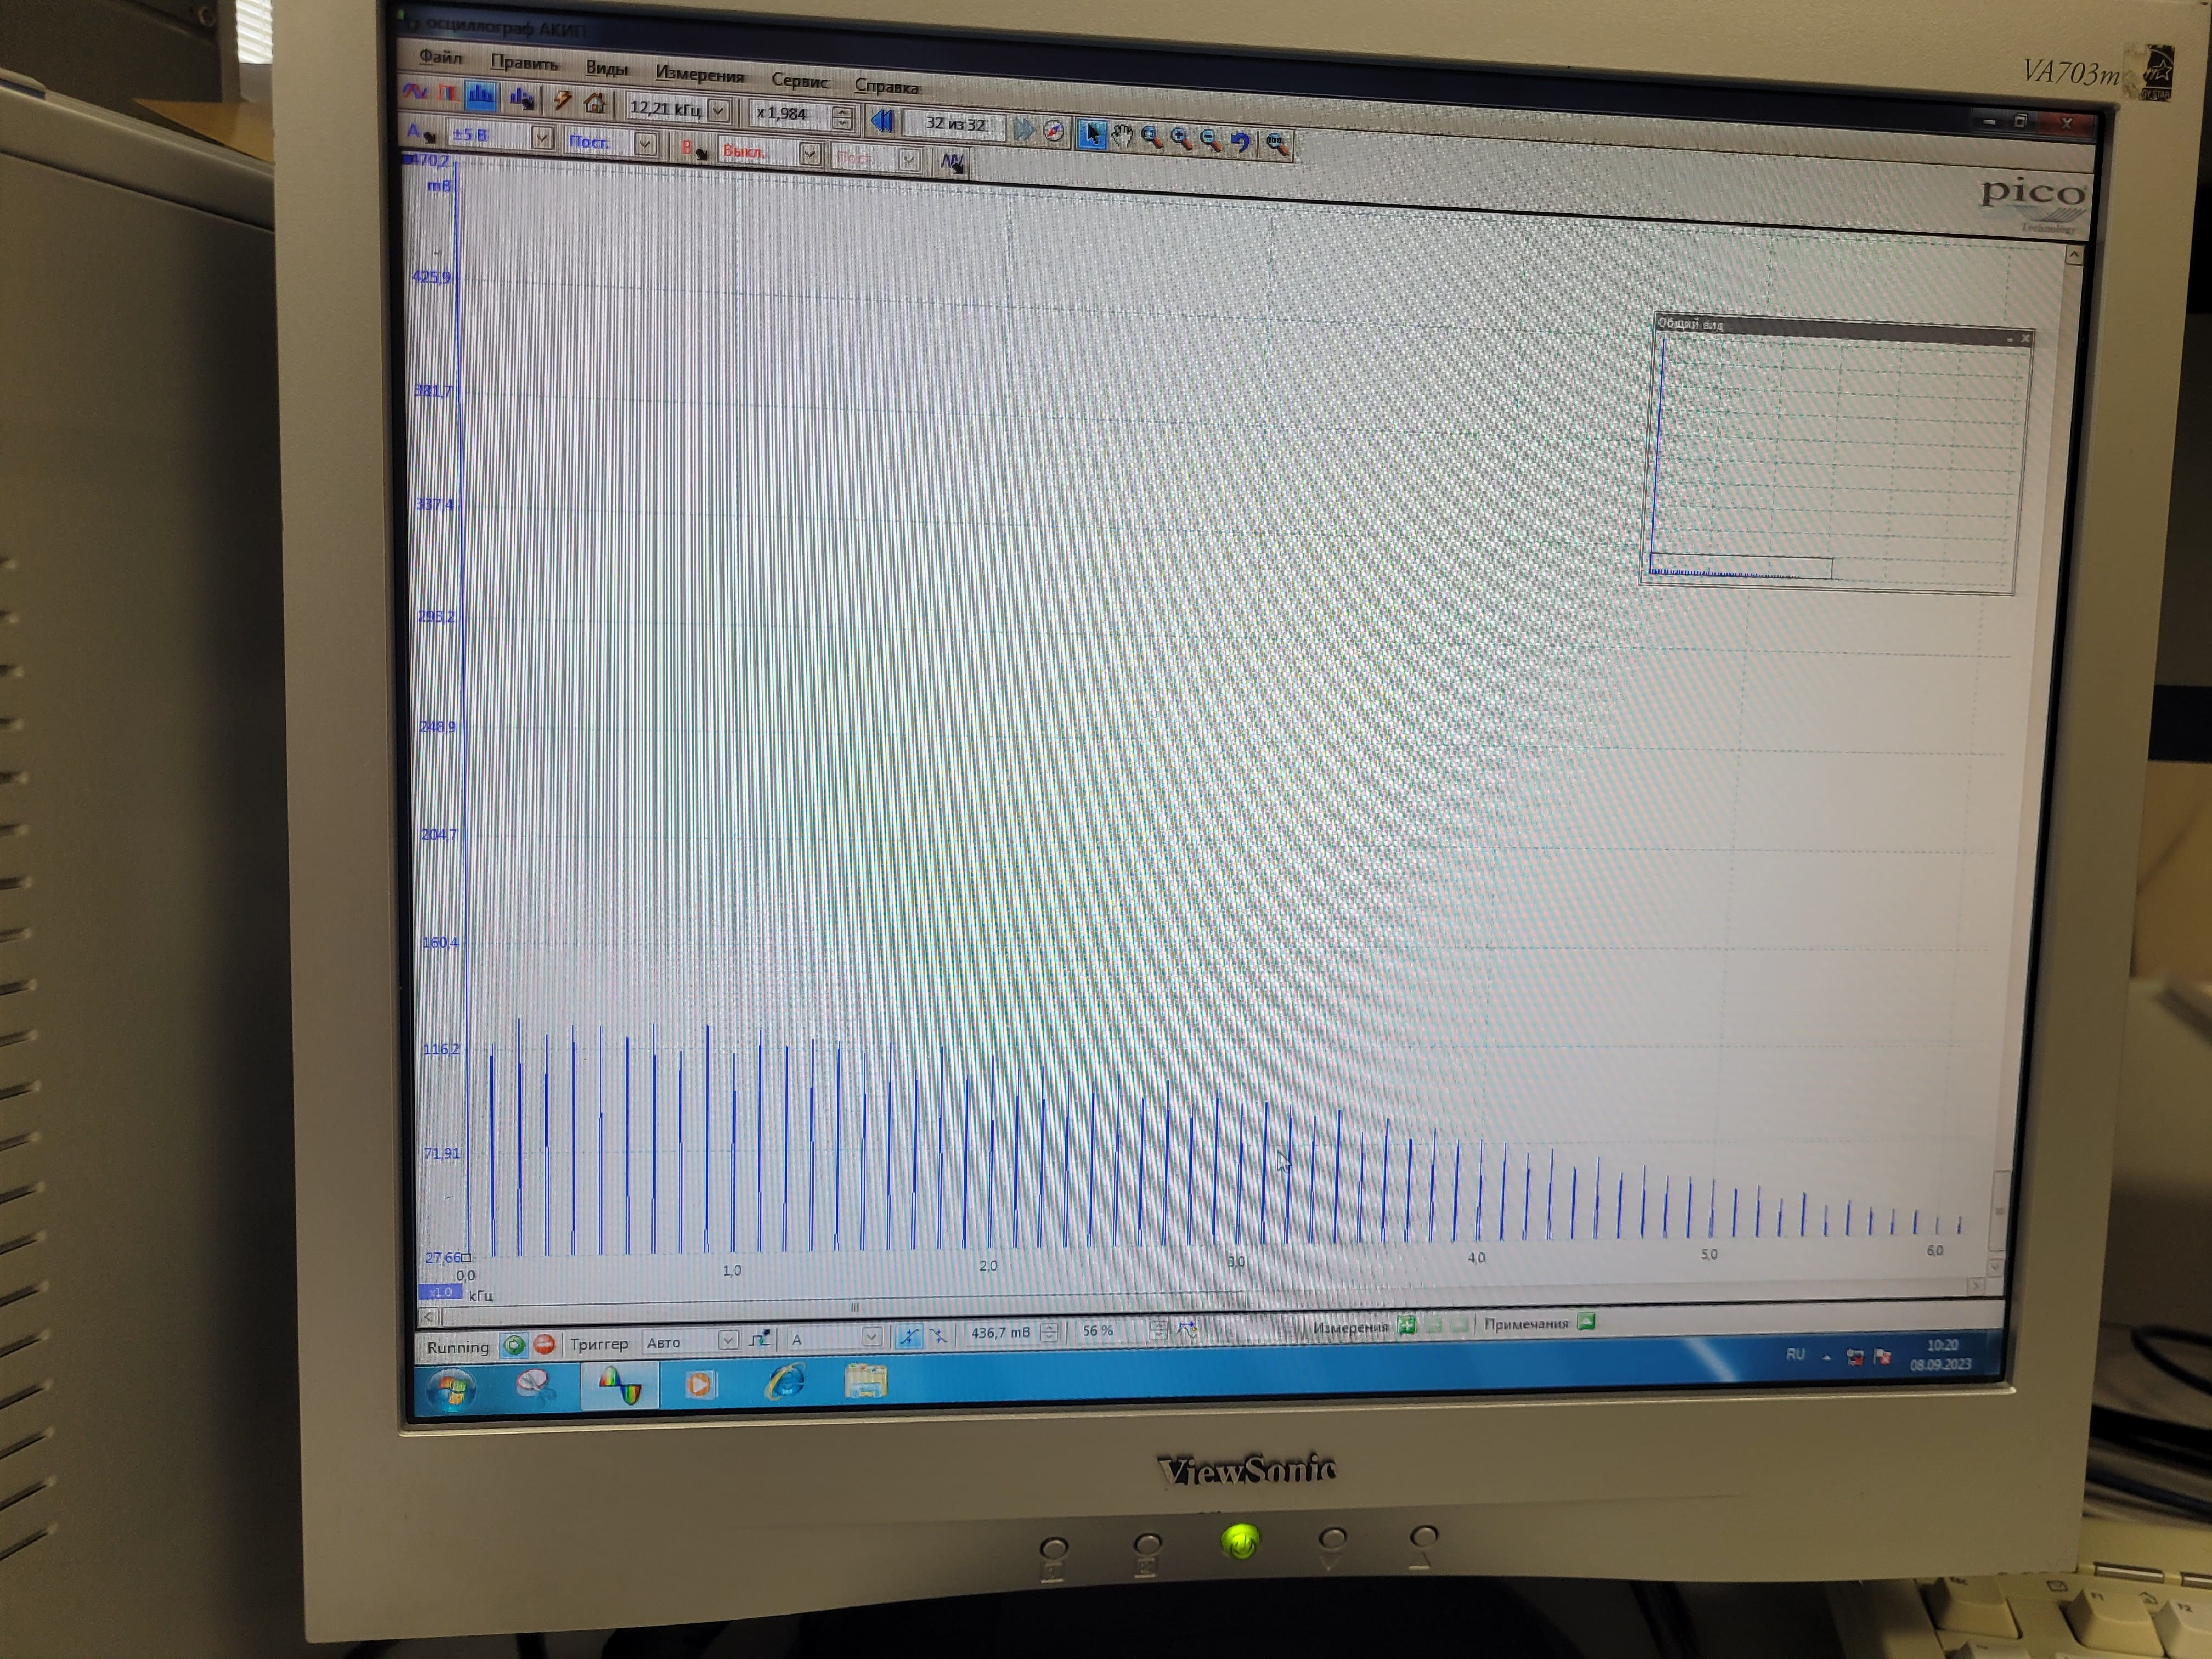
\includegraphics[width=1\linewidth]{V_3k_10T.jpg}} $\nu$ = 1 3Гц \\
% \end{minipage}
% \hfill
% \caption{}
% \label{ris:experimentalcorrelationsignals}
% \end{figure}


% \newpage

% \textbf{б.} Изменяем $T$ при фиксированных $\nu_0$ = 1 кГц.


% \begin{figure}[h]
% \begin{minipage}[h]{0.47\linewidth}
% \center{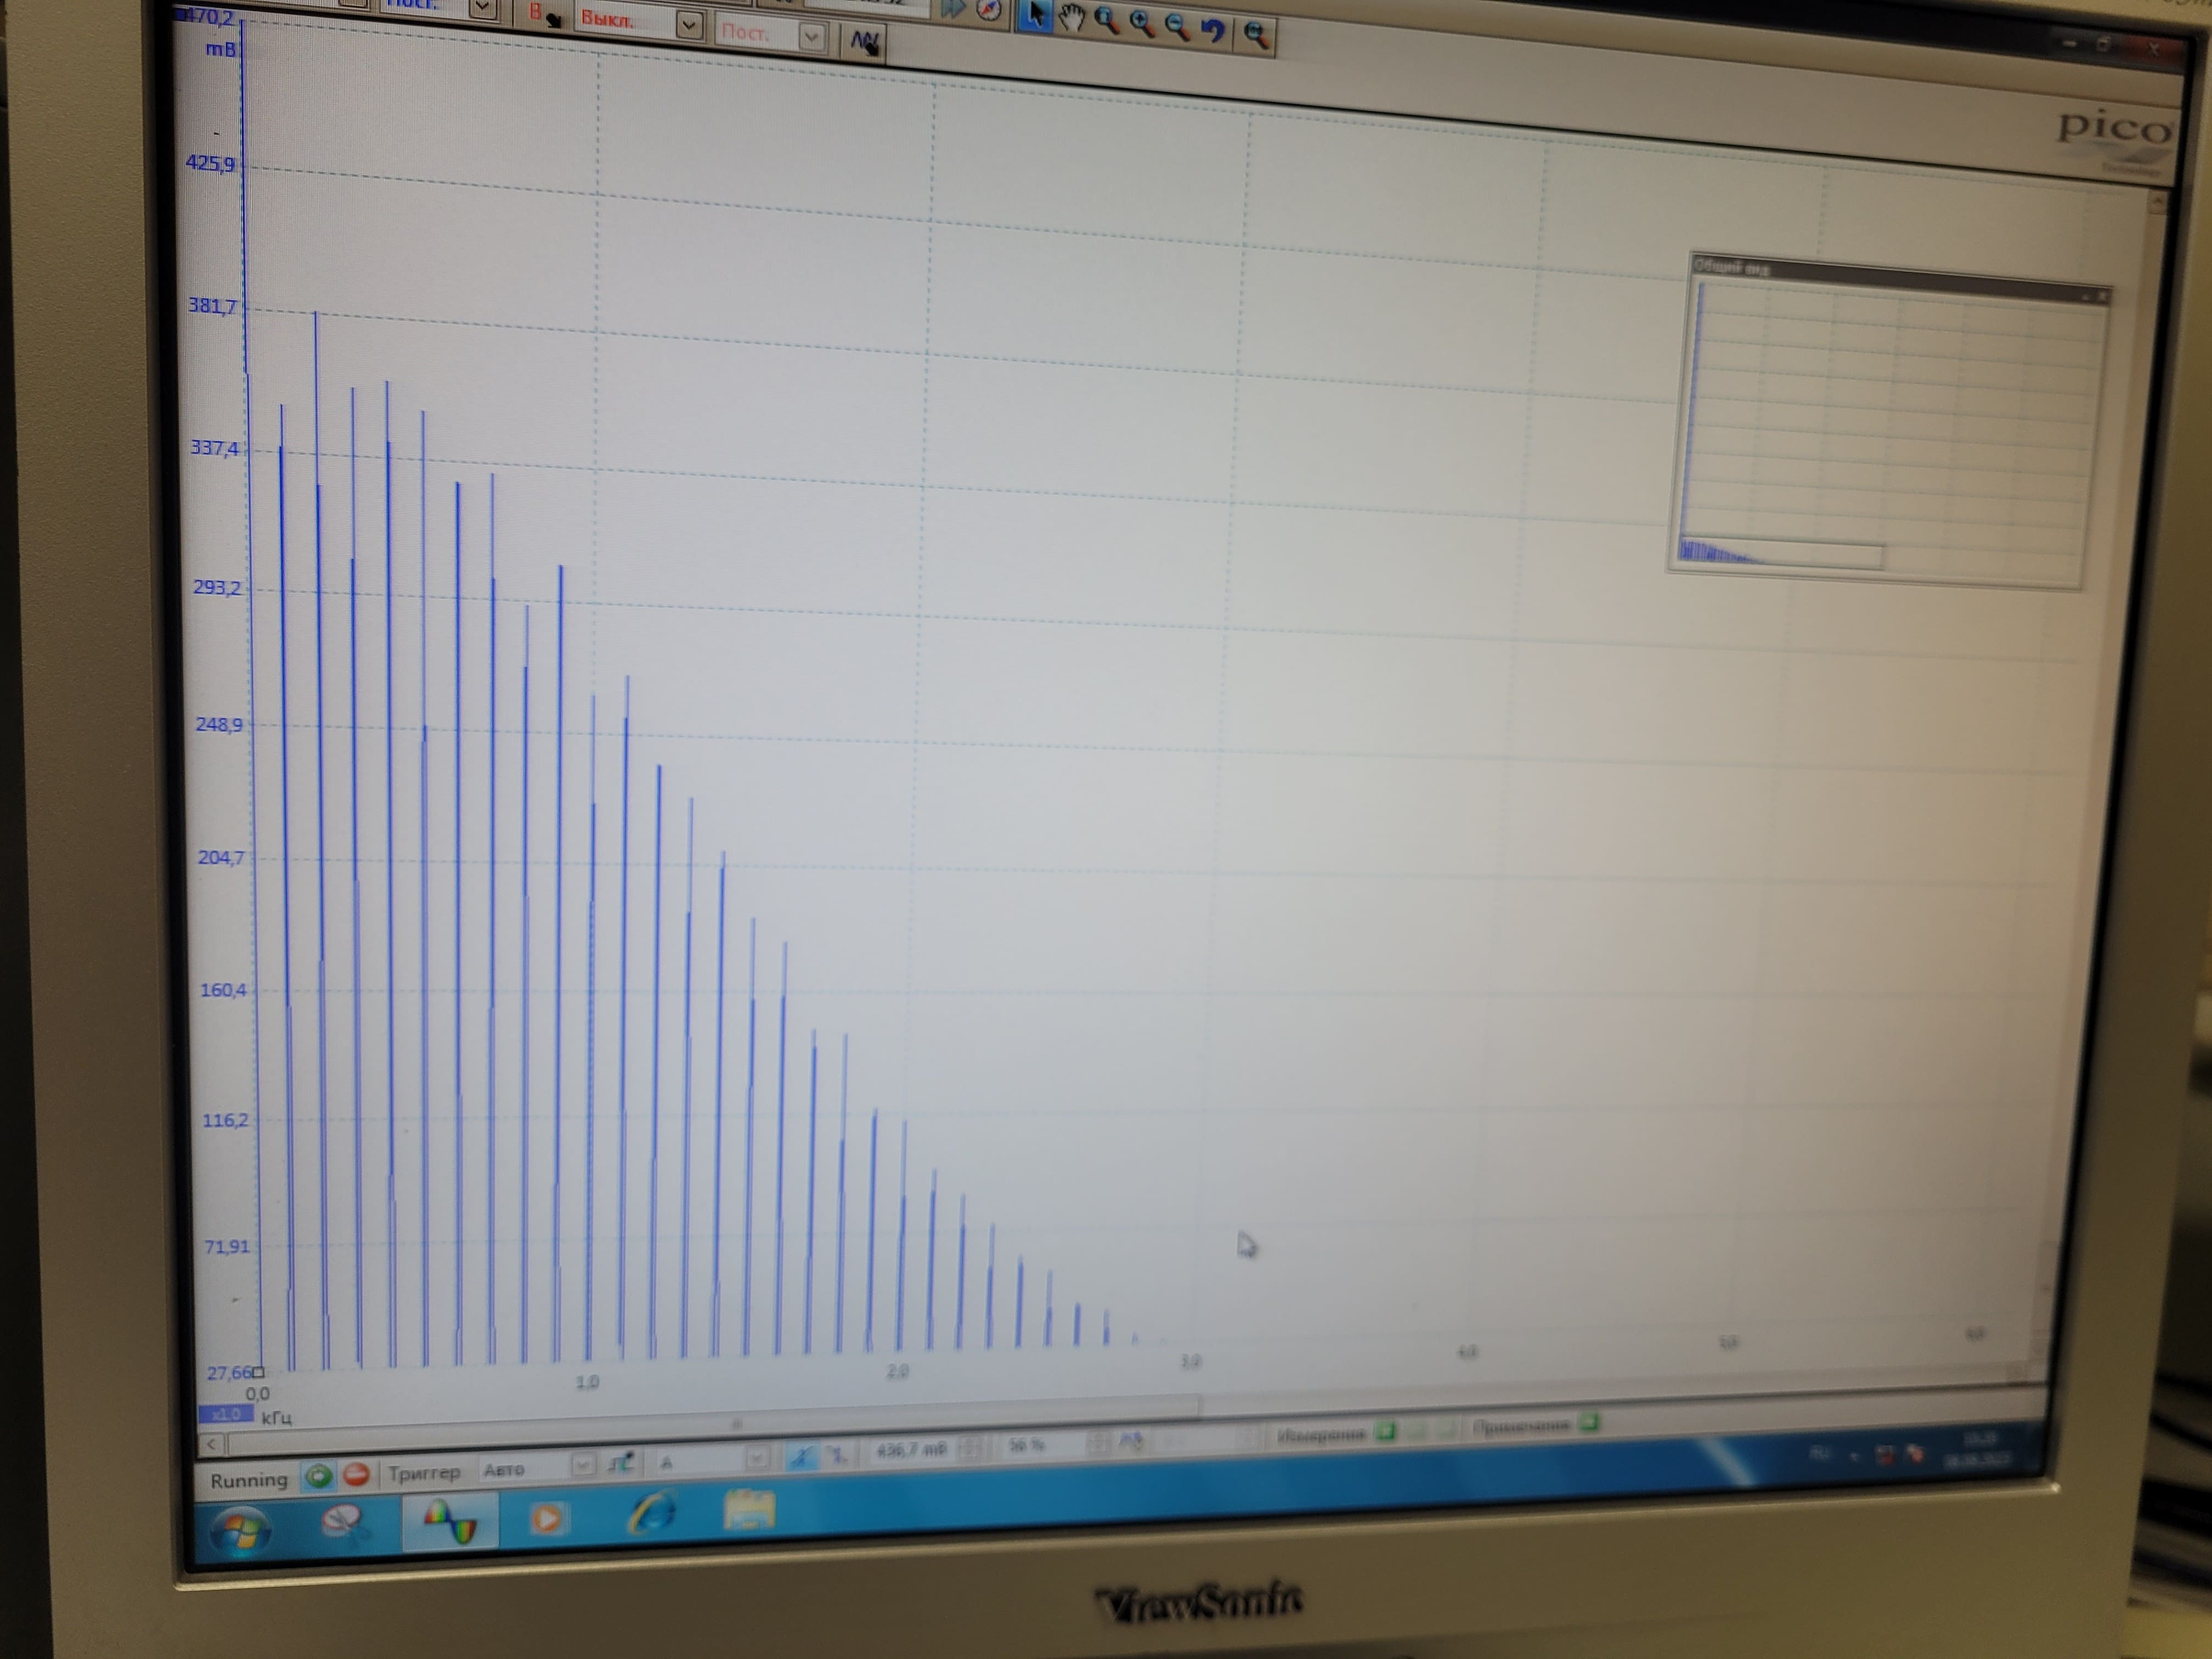
\includegraphics[width=1\linewidth]{V_1k_10T.jpg}} $T$ = 10 мс \\
% \end{minipage}
% \hfill
% \begin{minipage}[h]{0.47\linewidth}
% \center{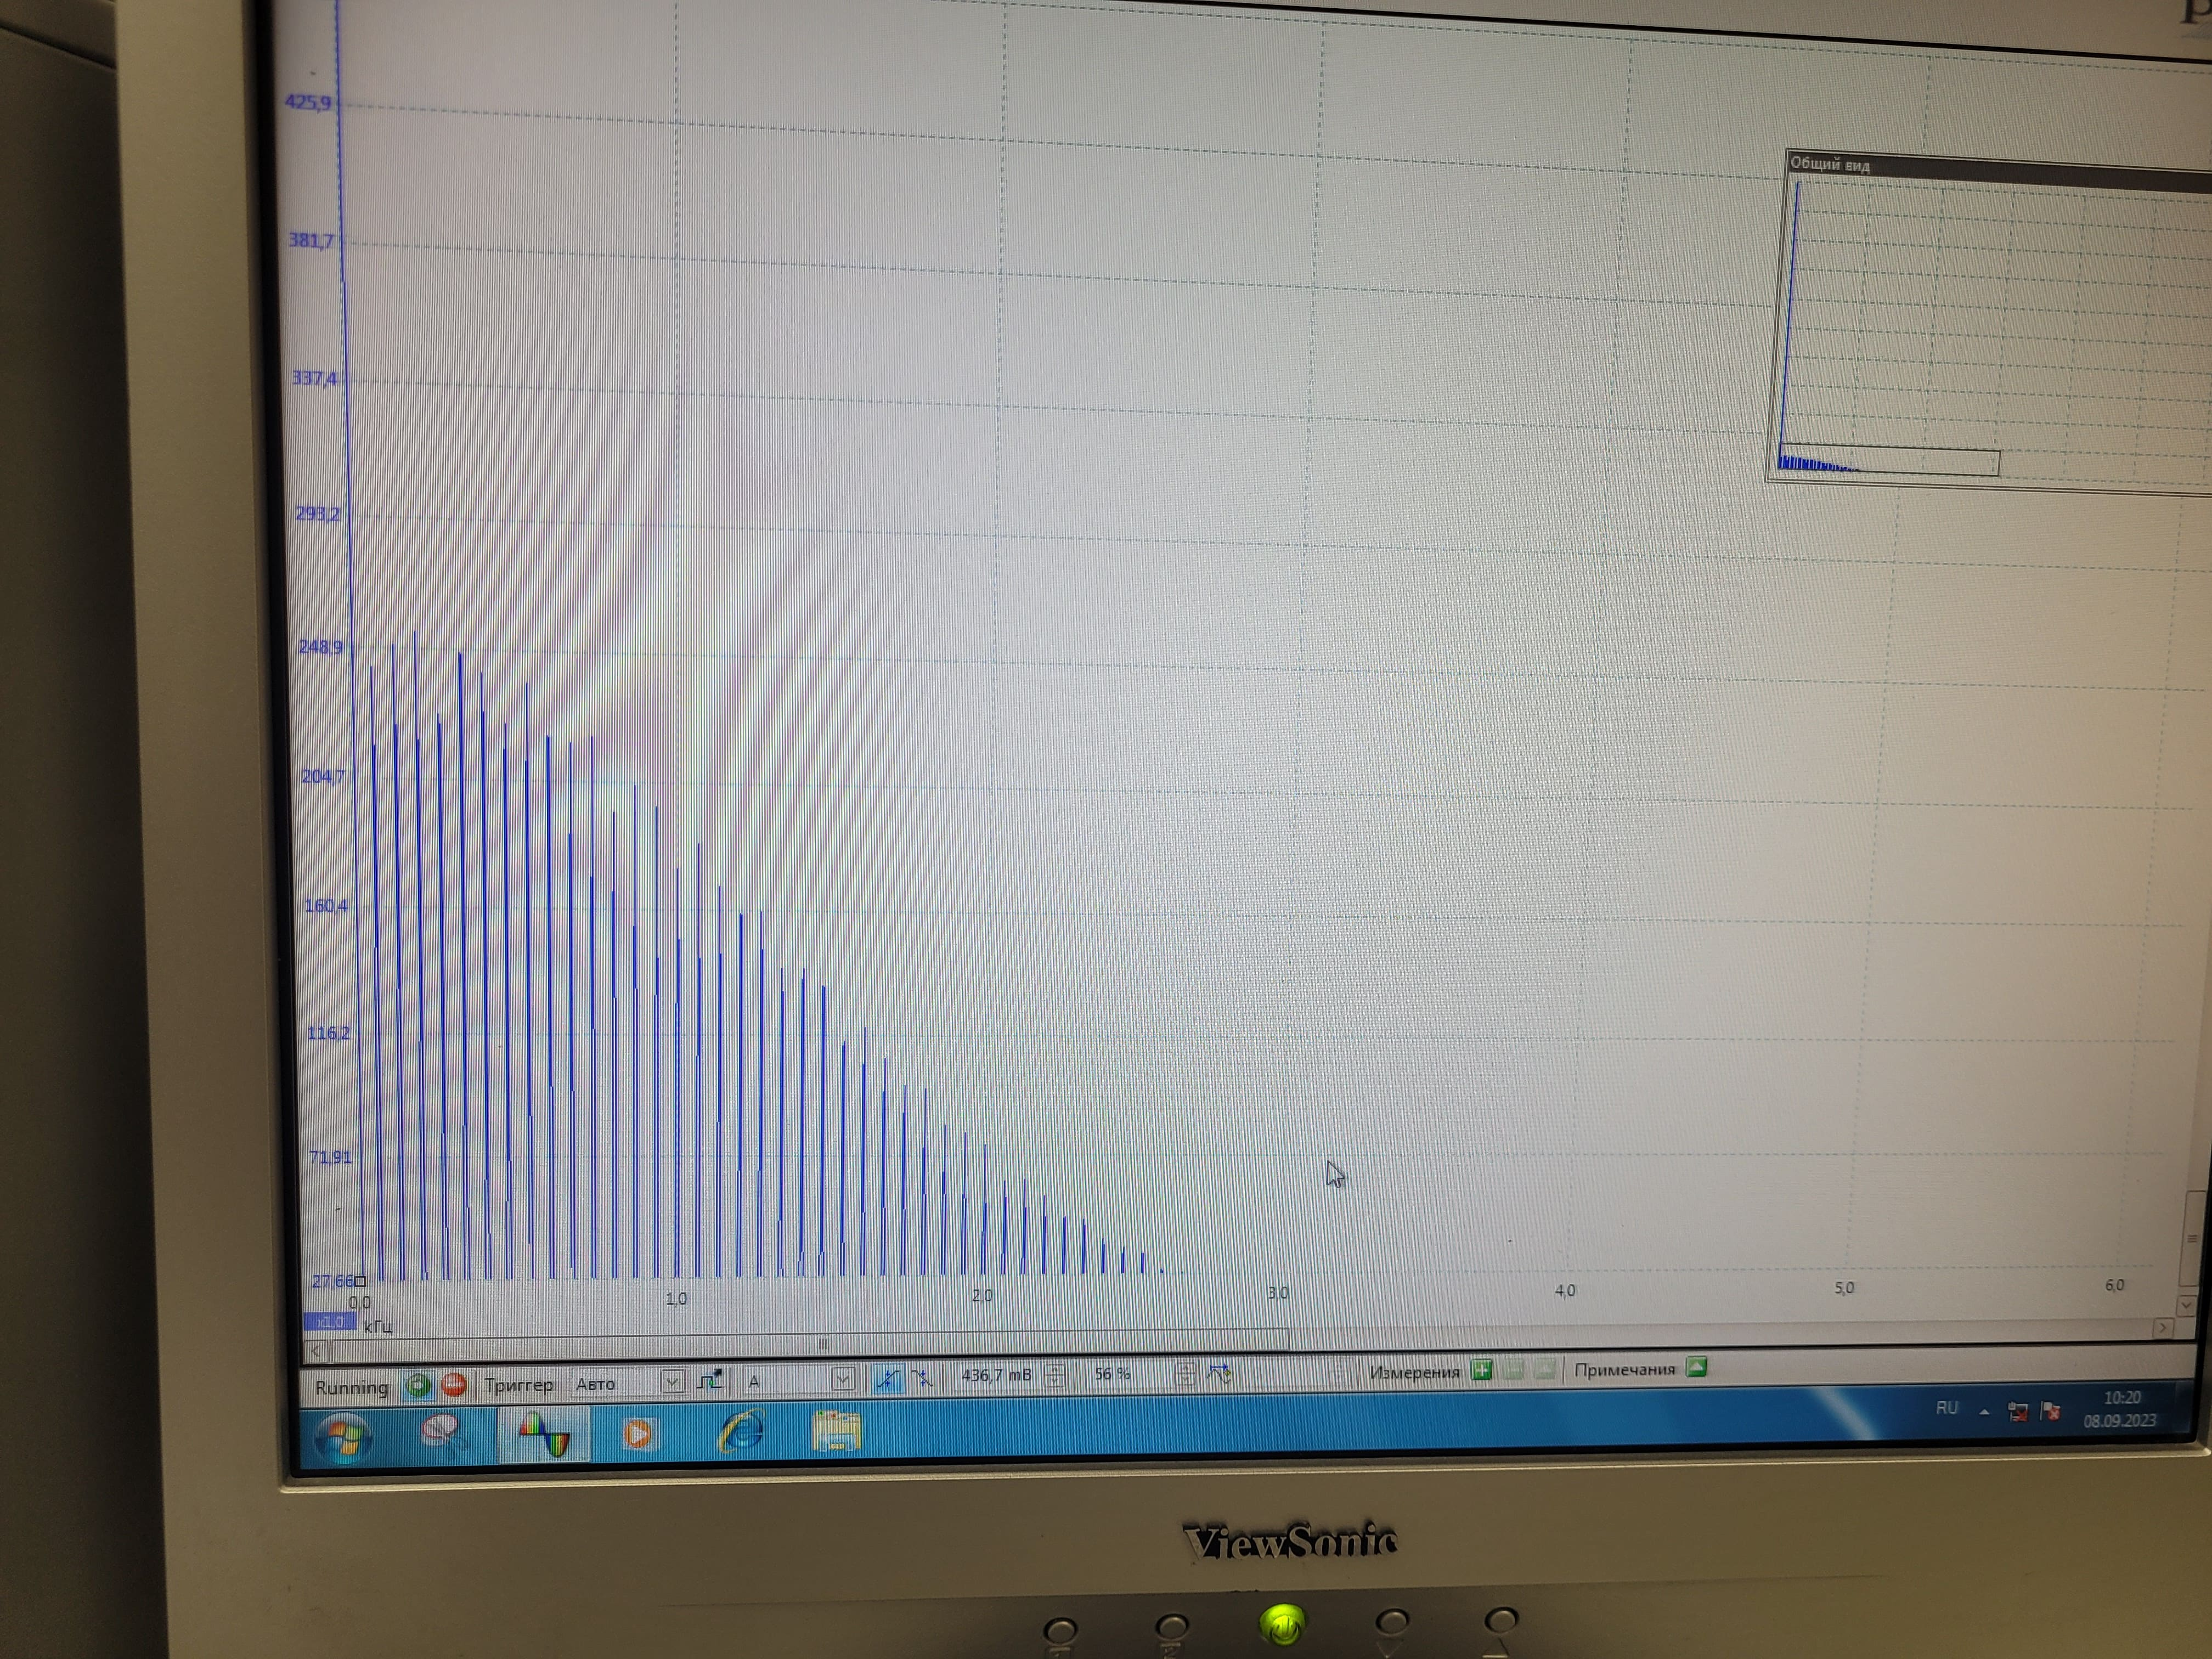
\includegraphics[width=1\linewidth]{V_1k_15T.jpg}} \\  $T$ = 15 мс
% \end{minipage}
% \vfill
% \begin{minipage}[h]{0.47\linewidth}
% \center{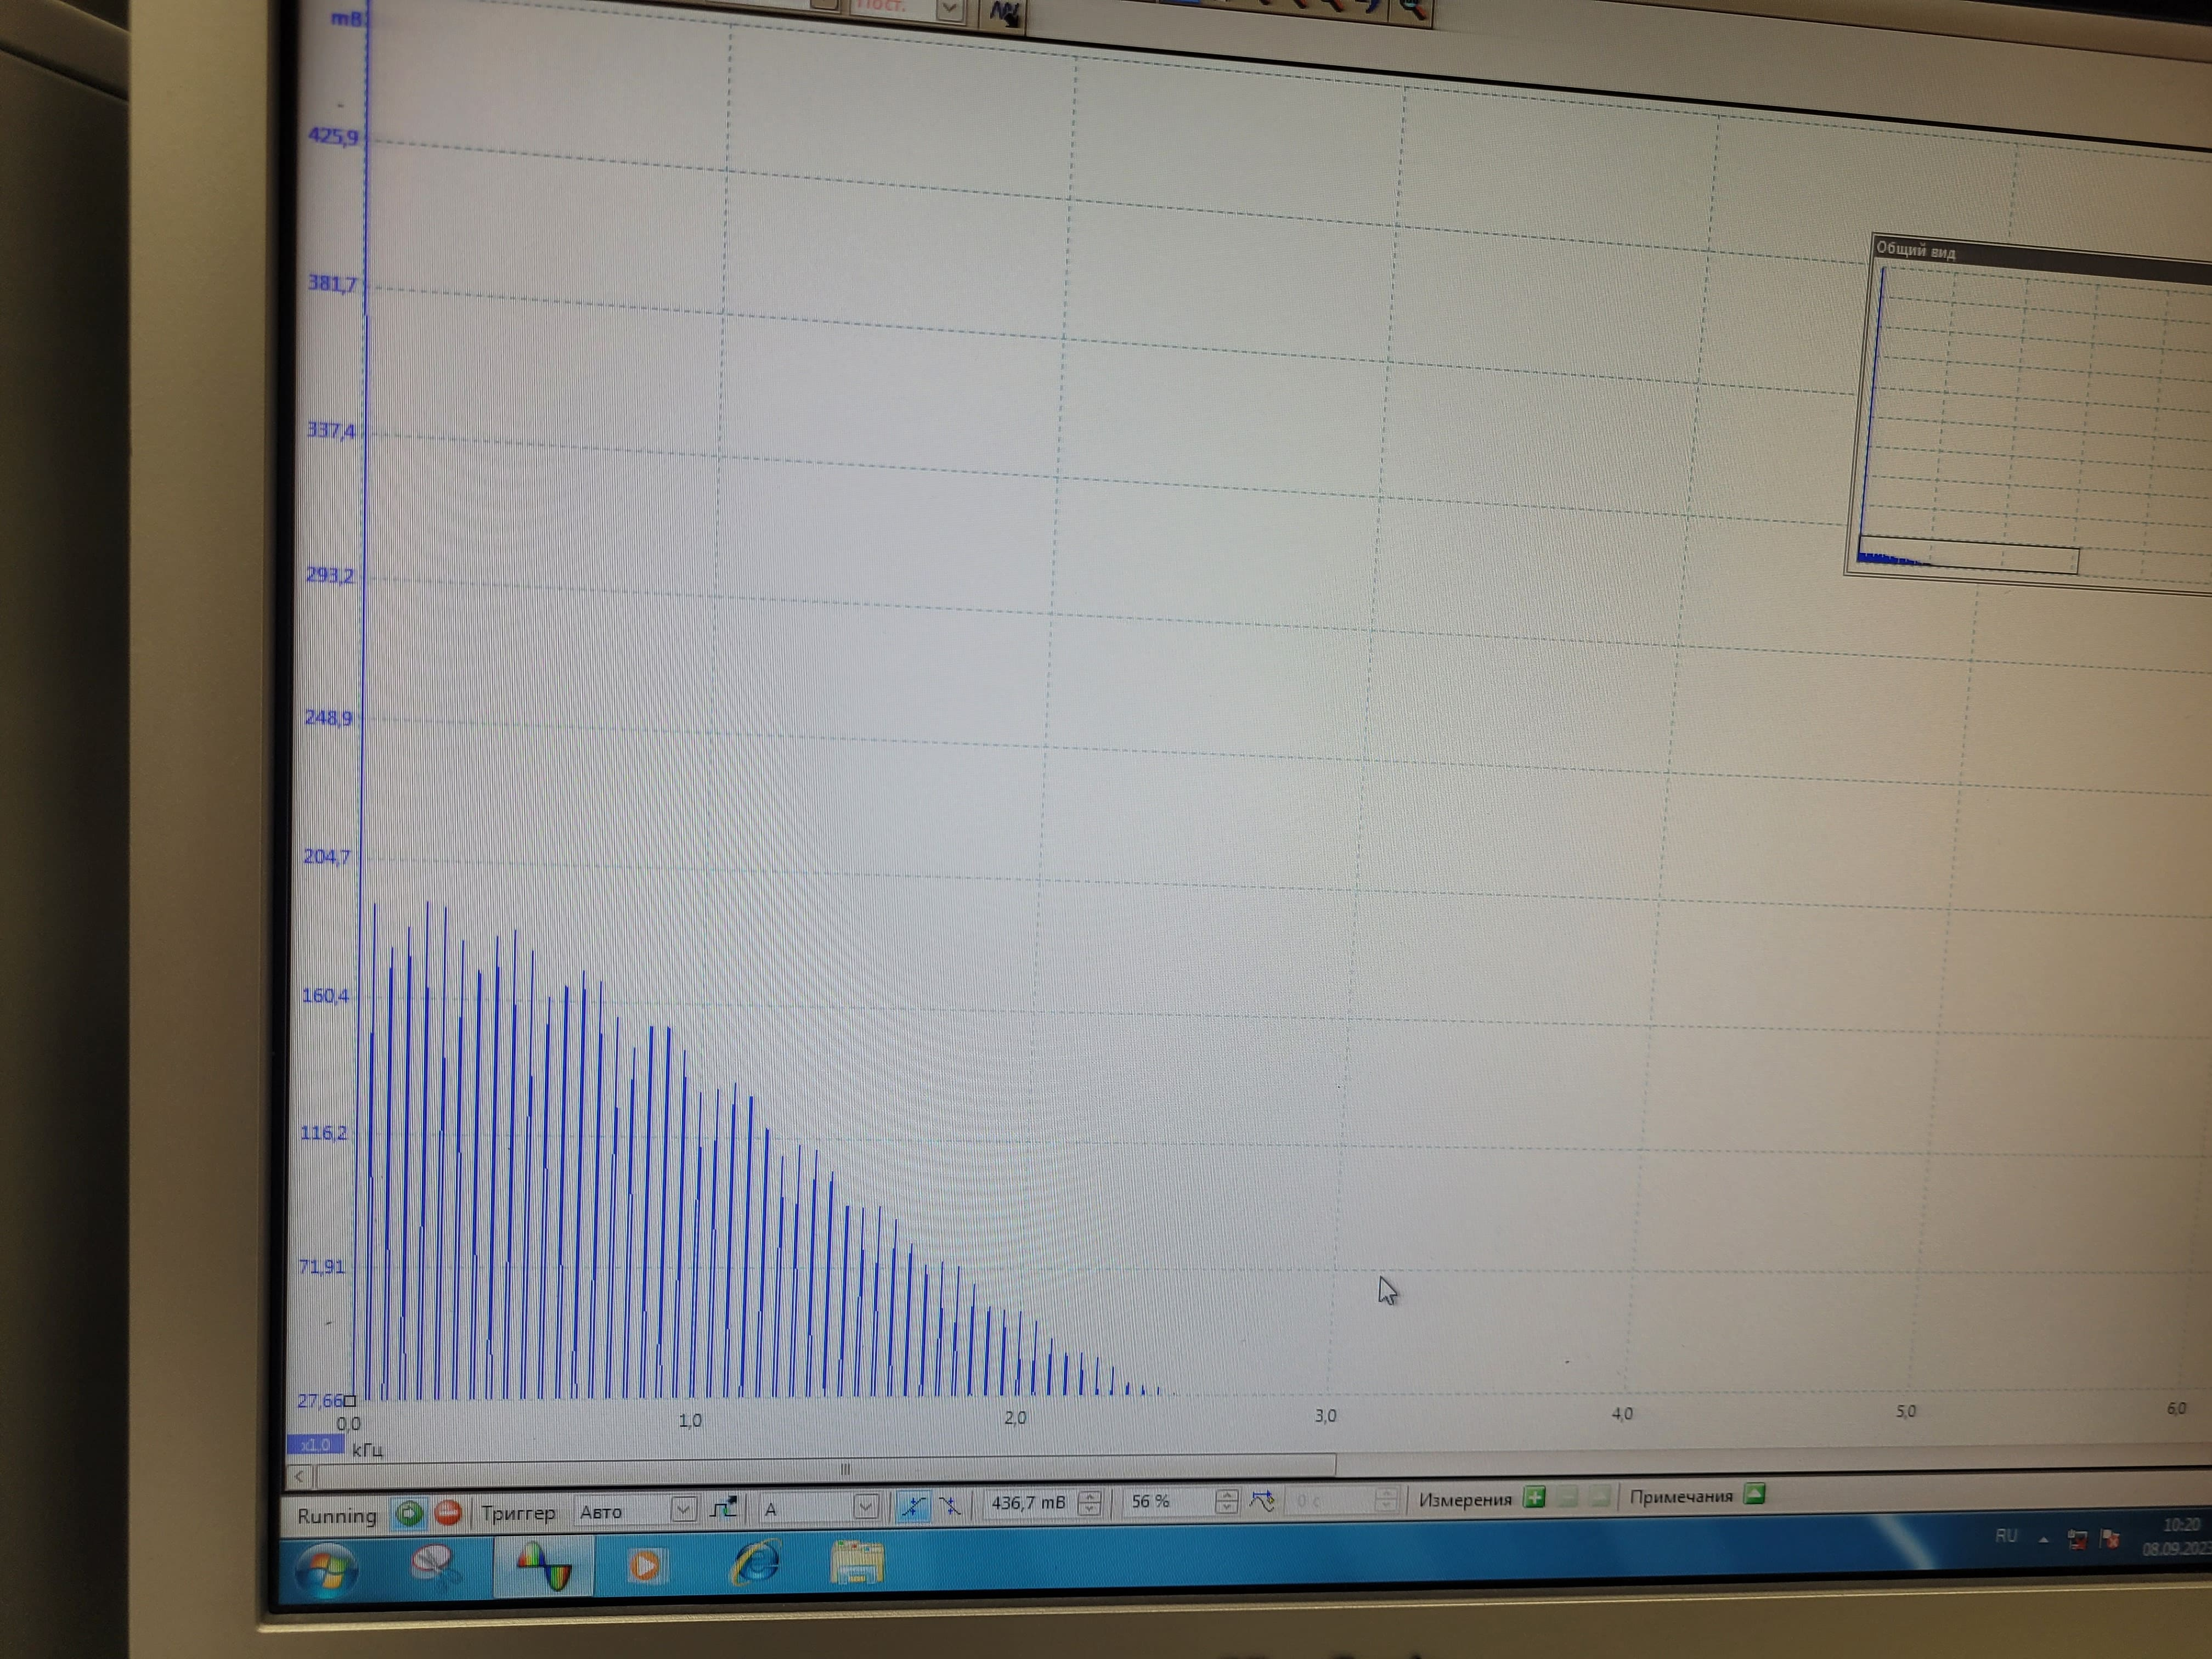
\includegraphics[width=1\linewidth]{V_1k_20T.jpg}} $T$ = 20 мс\\
% \end{minipage}
% \hfill
% \caption{}
% \label{ris:experimentalcorrelationsignals}
% \end{figure}

% \item [\textbf{3.}] Найдём ширину отдельного импульса $\tau$ и его спектра $\Delta \nu$:
% \begin{table}[h!]
%     \centering
%     \begin{tabular}{|c|c|c|}
% \hline
% $\nu$, кГц & 1 & 2 \\ \hline
% $\tau$, мкс & 299.5 & 148.2 \\ \hline
% $\frac{\Delta \nu}{2}$, кГц & 1.403 & 2.906 \\ \hline
% \end{tabular}
%     \caption{}
%     \label{table4}
% \end{table}
% \end{enumerate}

% Видно, что соотношение неопределённости выполняется, но численное значение отличается :
% $$\Delta \nu \cdot \tau = 1.403\cdot2\cdot10^3\cdot299.5\cdot10^\text{-6} = 0.84$$

% $$\Delta \nu \cdot \tau = 2.906\cdot2\cdot10^3\cdot148.2\cdot10^\text{-6} = 0.86$$


%\newpage

\subsection*{Г. Наблюдение спектра амплитудно-модулированного сигнала}


\begin{enumerate}


\item [\textbf{1.}] Настраиваем генератор в режим модулированного по амплитуде синусоидального сигнала с несущей частотой $\nu_0$ = 50 кГц, частотой модуляции $\nu_\text{мод}$ = 2 кГц и глубиной модуляции $m$ = 0.5.

\item [\textbf{2.}] Получаем на экране спектр (Преобразование Фурье) сигнала. Из графика получим $A_{max} = 3.057 \text{мВ}$ и $A_{min} = 1.027 \text{мВ}$ и убедимся в справедливости соотношения $$ m = \frac{A_\text{max} - A_\text{min}}{A_\text{max} + A_\text{min}} = \frac{2.03}{4.084} \approx 0.5 $$
Поскольку мы установили глубину модуляции на $0,5$, а из теории у нас получилась $0,497$, то мы видим, что формула \ref{eq8} верна.

\item [\textbf{3.}]
Изменяя на генераторе глубину модуляции $m$ в диапазоне от 10 \% до 100 \% (всего 6-8 точек), измерим отношение амплитуд боковой и основной
спектральных линий $a_{\text{бок}}/a_{\text{осн}}$. Построим график зависимости $a_{\text{бок}}/a_{\text{осн}}$ от $m$ и проверим, совпадает ли
результат с теоретическим.

\begin{center}
\begin{tabular}{|c|c|c|c|c|c|c|c|}
\hline
$m$, \% & 10 & 20 & 30 & 40 & 50 & 80 & 100 \\ \hline
$a_{\text{бок}}$, мВ & 69.02 & 136.3 & 207.1 & 283.2 & 352.2 & 559.2 & 669.0 \\ \hline
\multicolumn{8}{|c|}{$a_{\text{осн}}$ = 1318 мВ} \\ \hline
$a_{\text{бок}}/a_{\text{осн}}$ & 0.05 & 0.10 & 0.16 & 0.21 & 0.27 & 0.42 & 0.51 \\ \hline
\end{tabular}

\textbf{Таблица 3.} Исследование зависимости $a_{\text{бок}}/a_{\text{осн}}$ от $m$.
\end{center}
\begin{figure}[h]
    \centering
    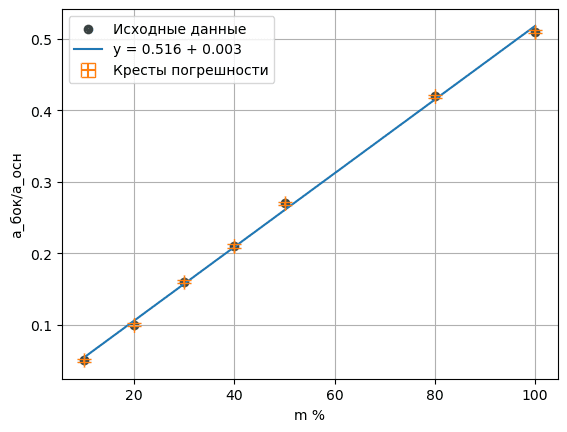
\includegraphics[width=0.7\linewidth]{grafic3.png}
    \caption{Зависимость $a_{\text{бок}}/a_{\text{осн}}$ от $m$}
    \label{grafic3}
\end{figure}
Построим график $\frac{a_{\text{бок}}}{a_{\text{осн}}}(m)$. Используя МНК, получим $k=0.516x\pm0,00007$, что подтверждает $\frac{a_{\text{бок}}}{a_{\text{осн}}}=\frac{m}{2}$, т.е. совпадает с теоретическим предсказанием. График приведён на рис.\ref{grafic3}.




\end{enumerate}








\newpage



\subsection*{Д. Наблюдение спектра сигнала, модулированного по фазе}



\begin{enumerate}


\item [\textbf{1.}] Настраиваем генератор в режим модулированного по фазе синусоидального сигнала с несущей частотой $\nu_0$ = 50 кГц, частотой модуляции $\nu_\text{мод}$ = 2 кГц и максимальным отклонением (глубиной модуляцией) $\varphi$ = 10$\degree$.

\item [\textbf{2.}] Получаем на экране спектр (Преобразование Фурье) сигнала.

\begin{figure}[h]
\begin{minipage}[h]{0.44\linewidth}
\center{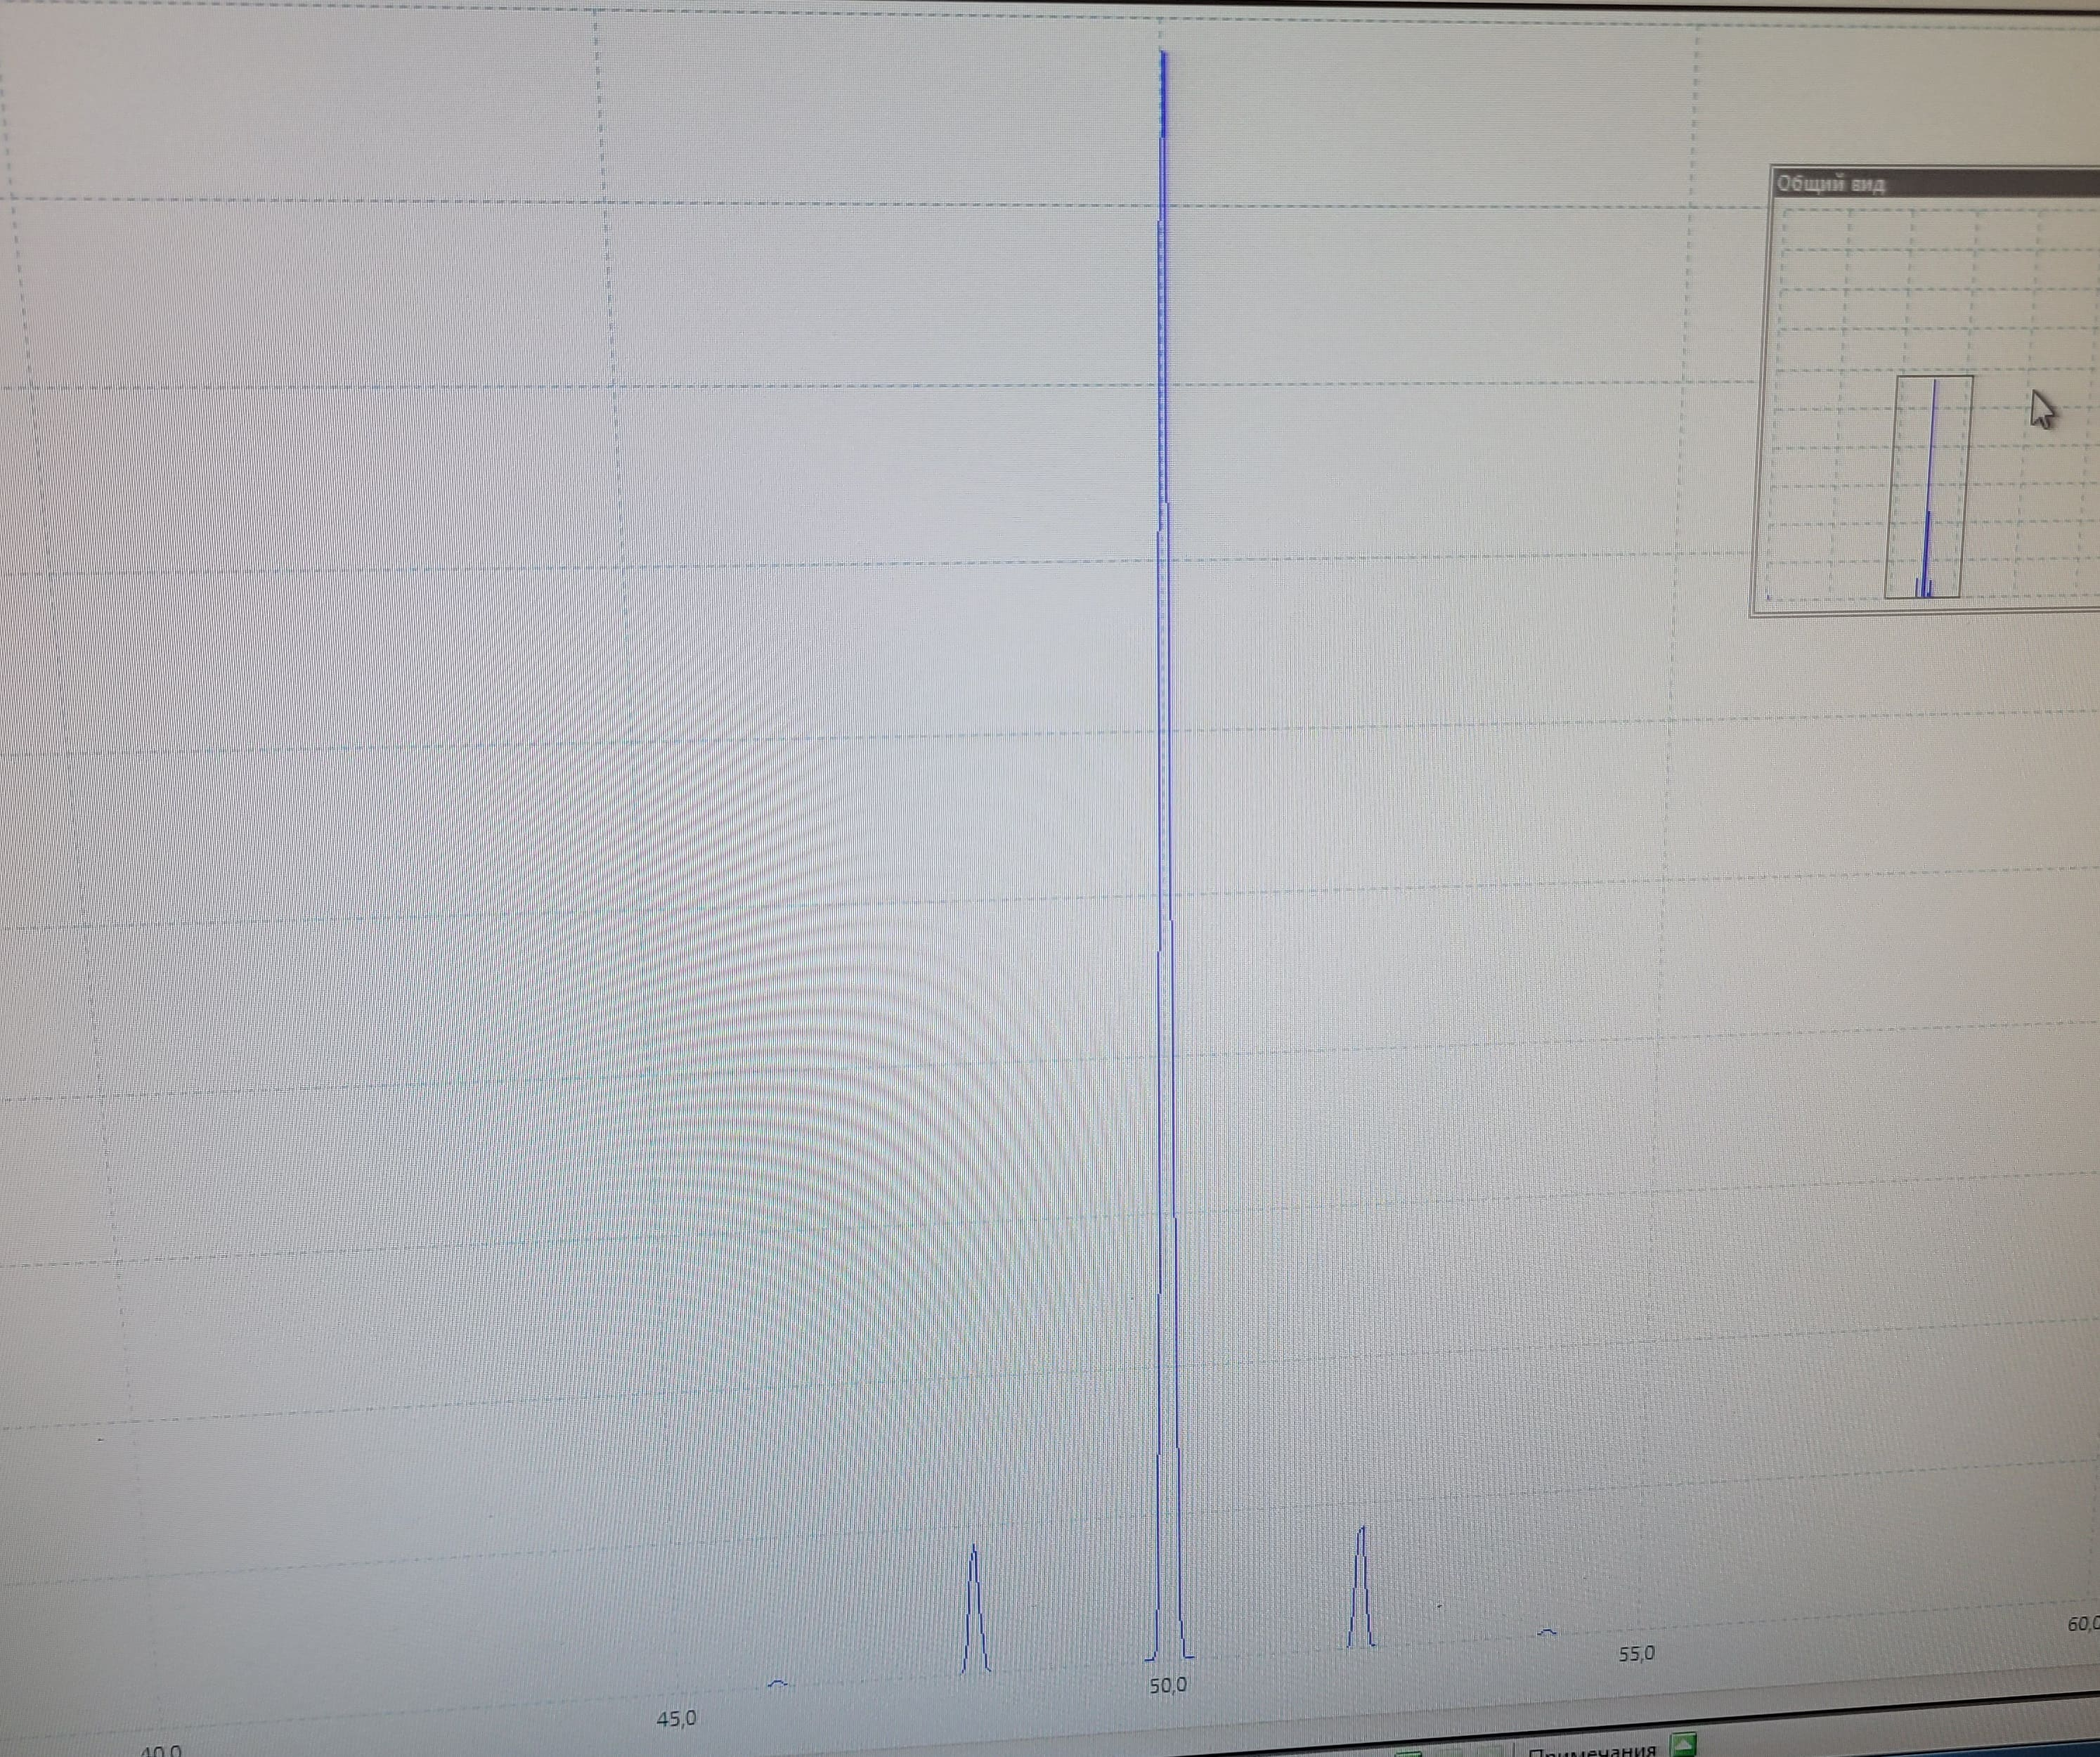
\includegraphics[width=1\linewidth]{D_50k_2k_10f.jpg}} $\nu_0$ = 50 кГц, $\nu_\text{мод}$ = 2 кГц, $\varphi$ = 10$\degree$  \\
\end{minipage}
\hfill
\begin{minipage}[h]{0.44\linewidth}
\center{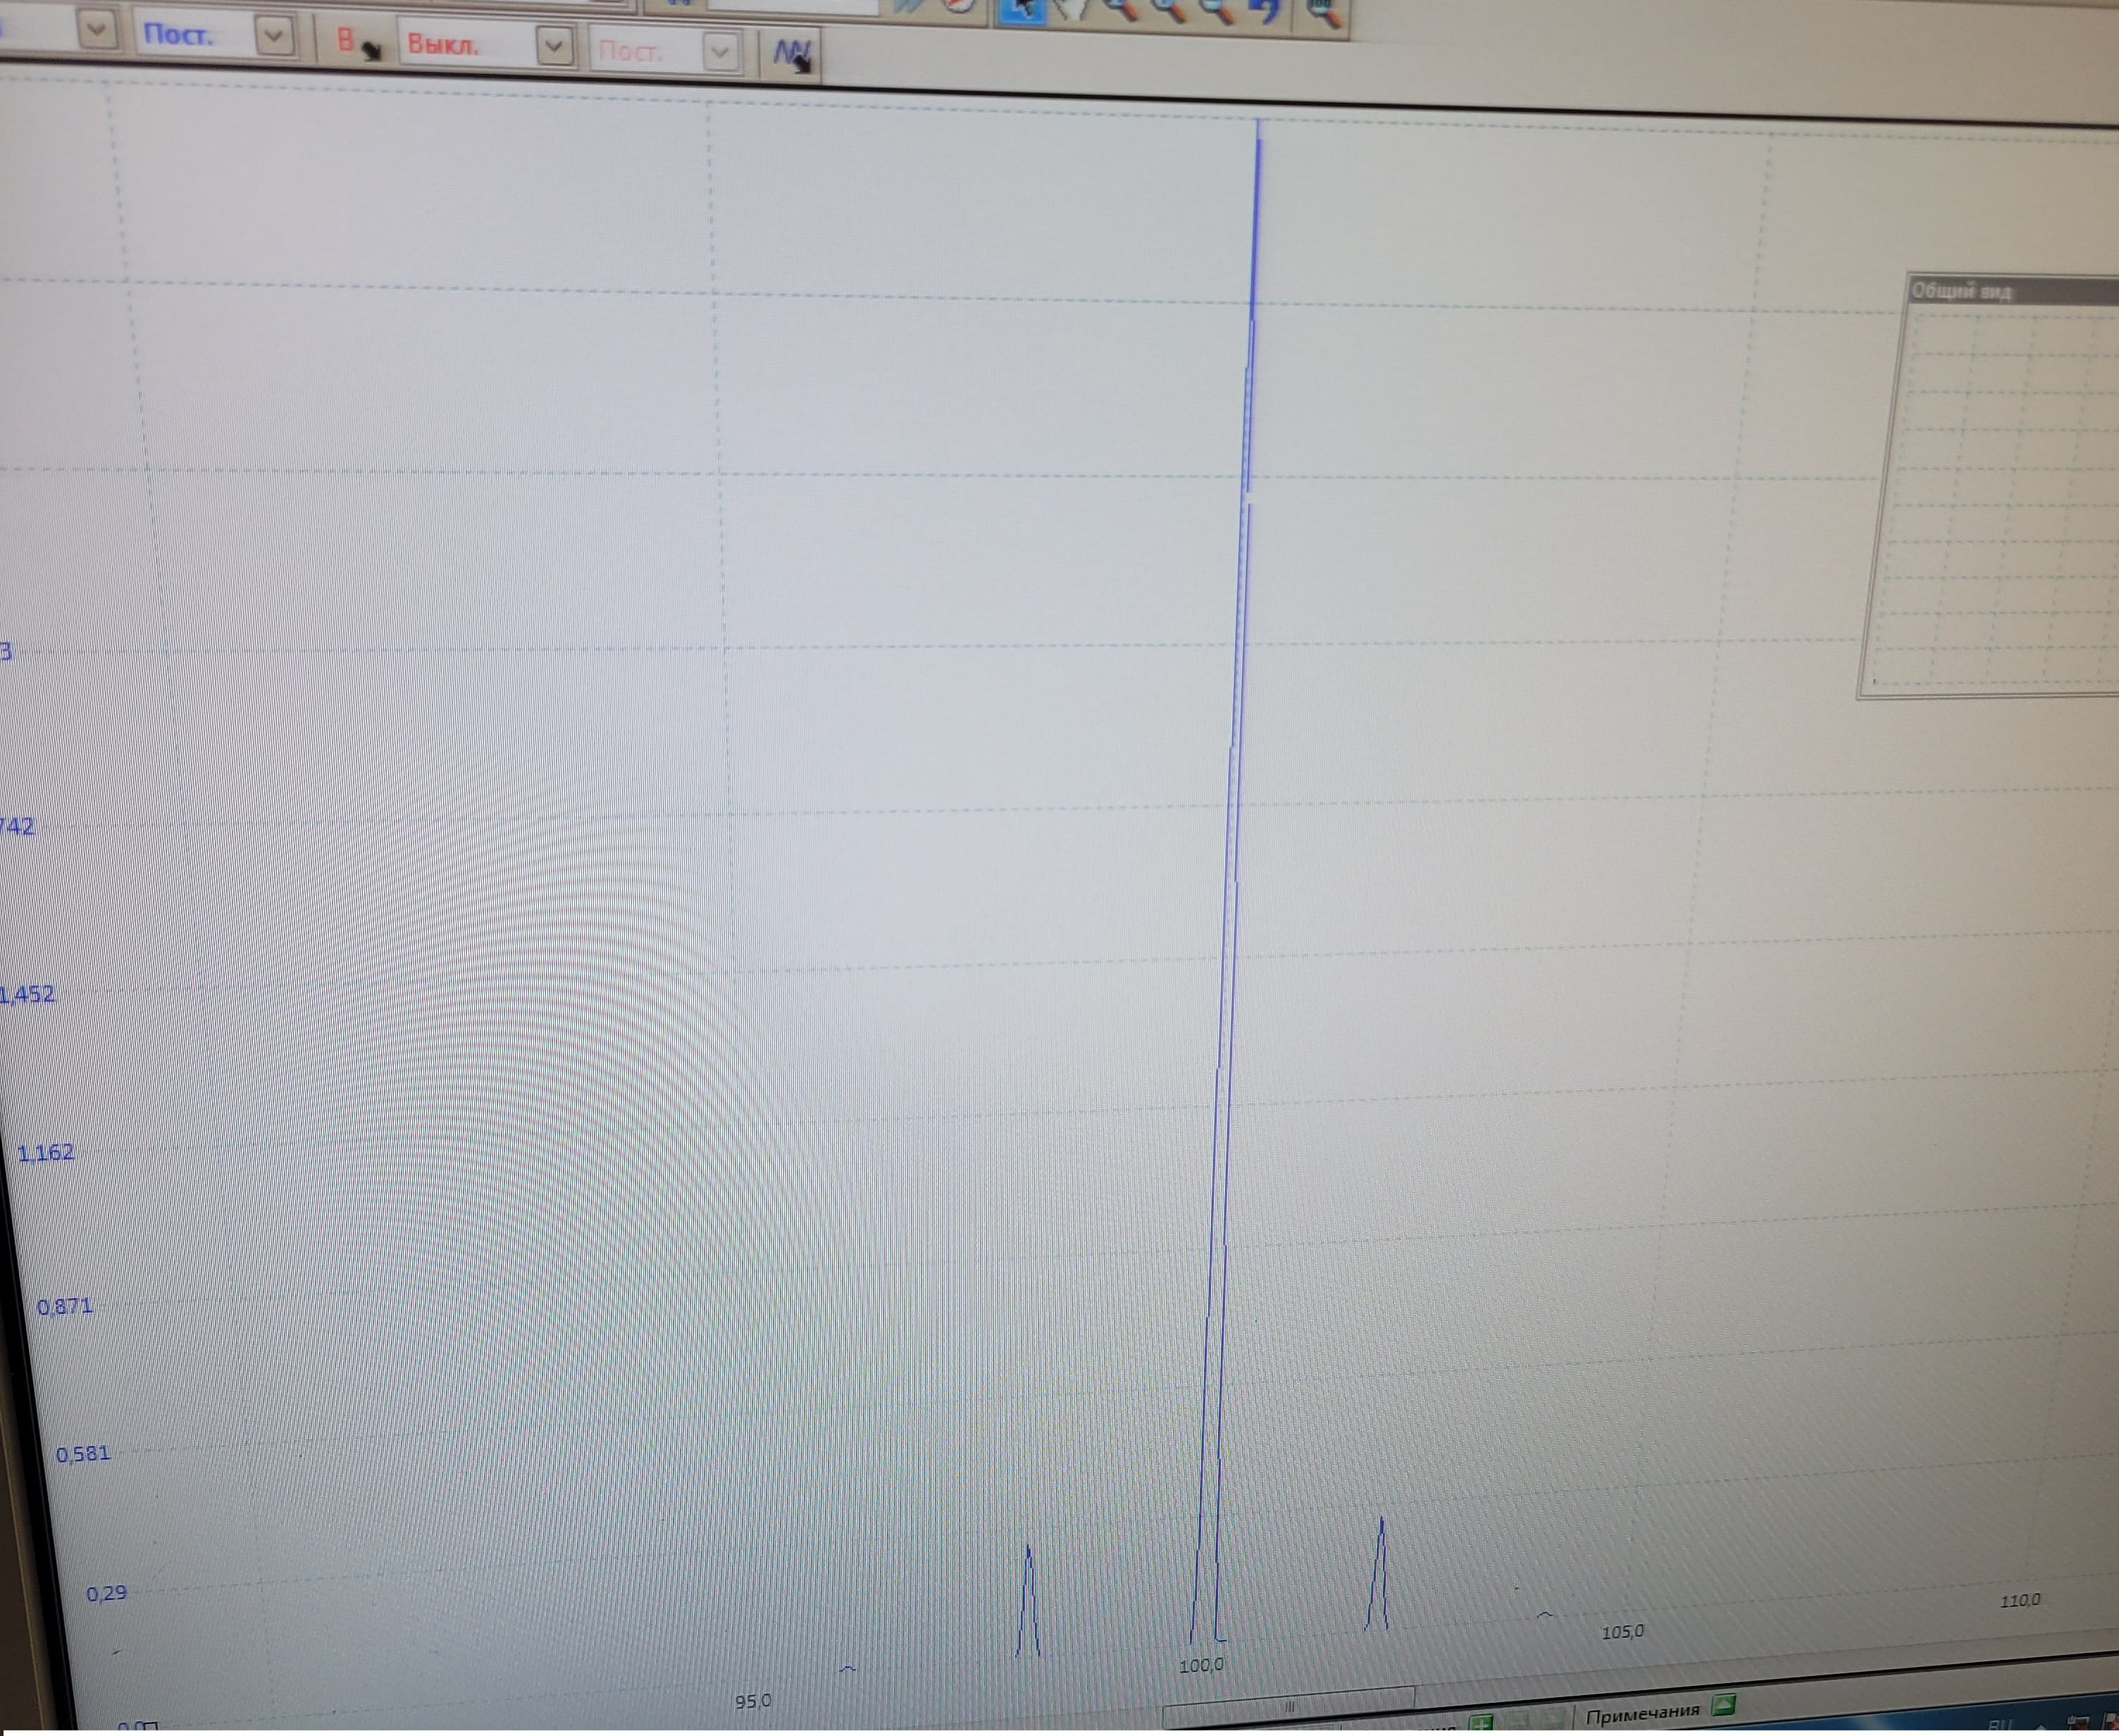
\includegraphics[width=1\linewidth]{D_100k_2k_10f.jpg}} \\  $\nu_0$ = 100 кГц, $\nu_\text{мод}$ = 2 кГц, $\varphi$ = 10$\degree$
\end{minipage}
\vfill
\begin{minipage}[h]{0.44\linewidth}
\center{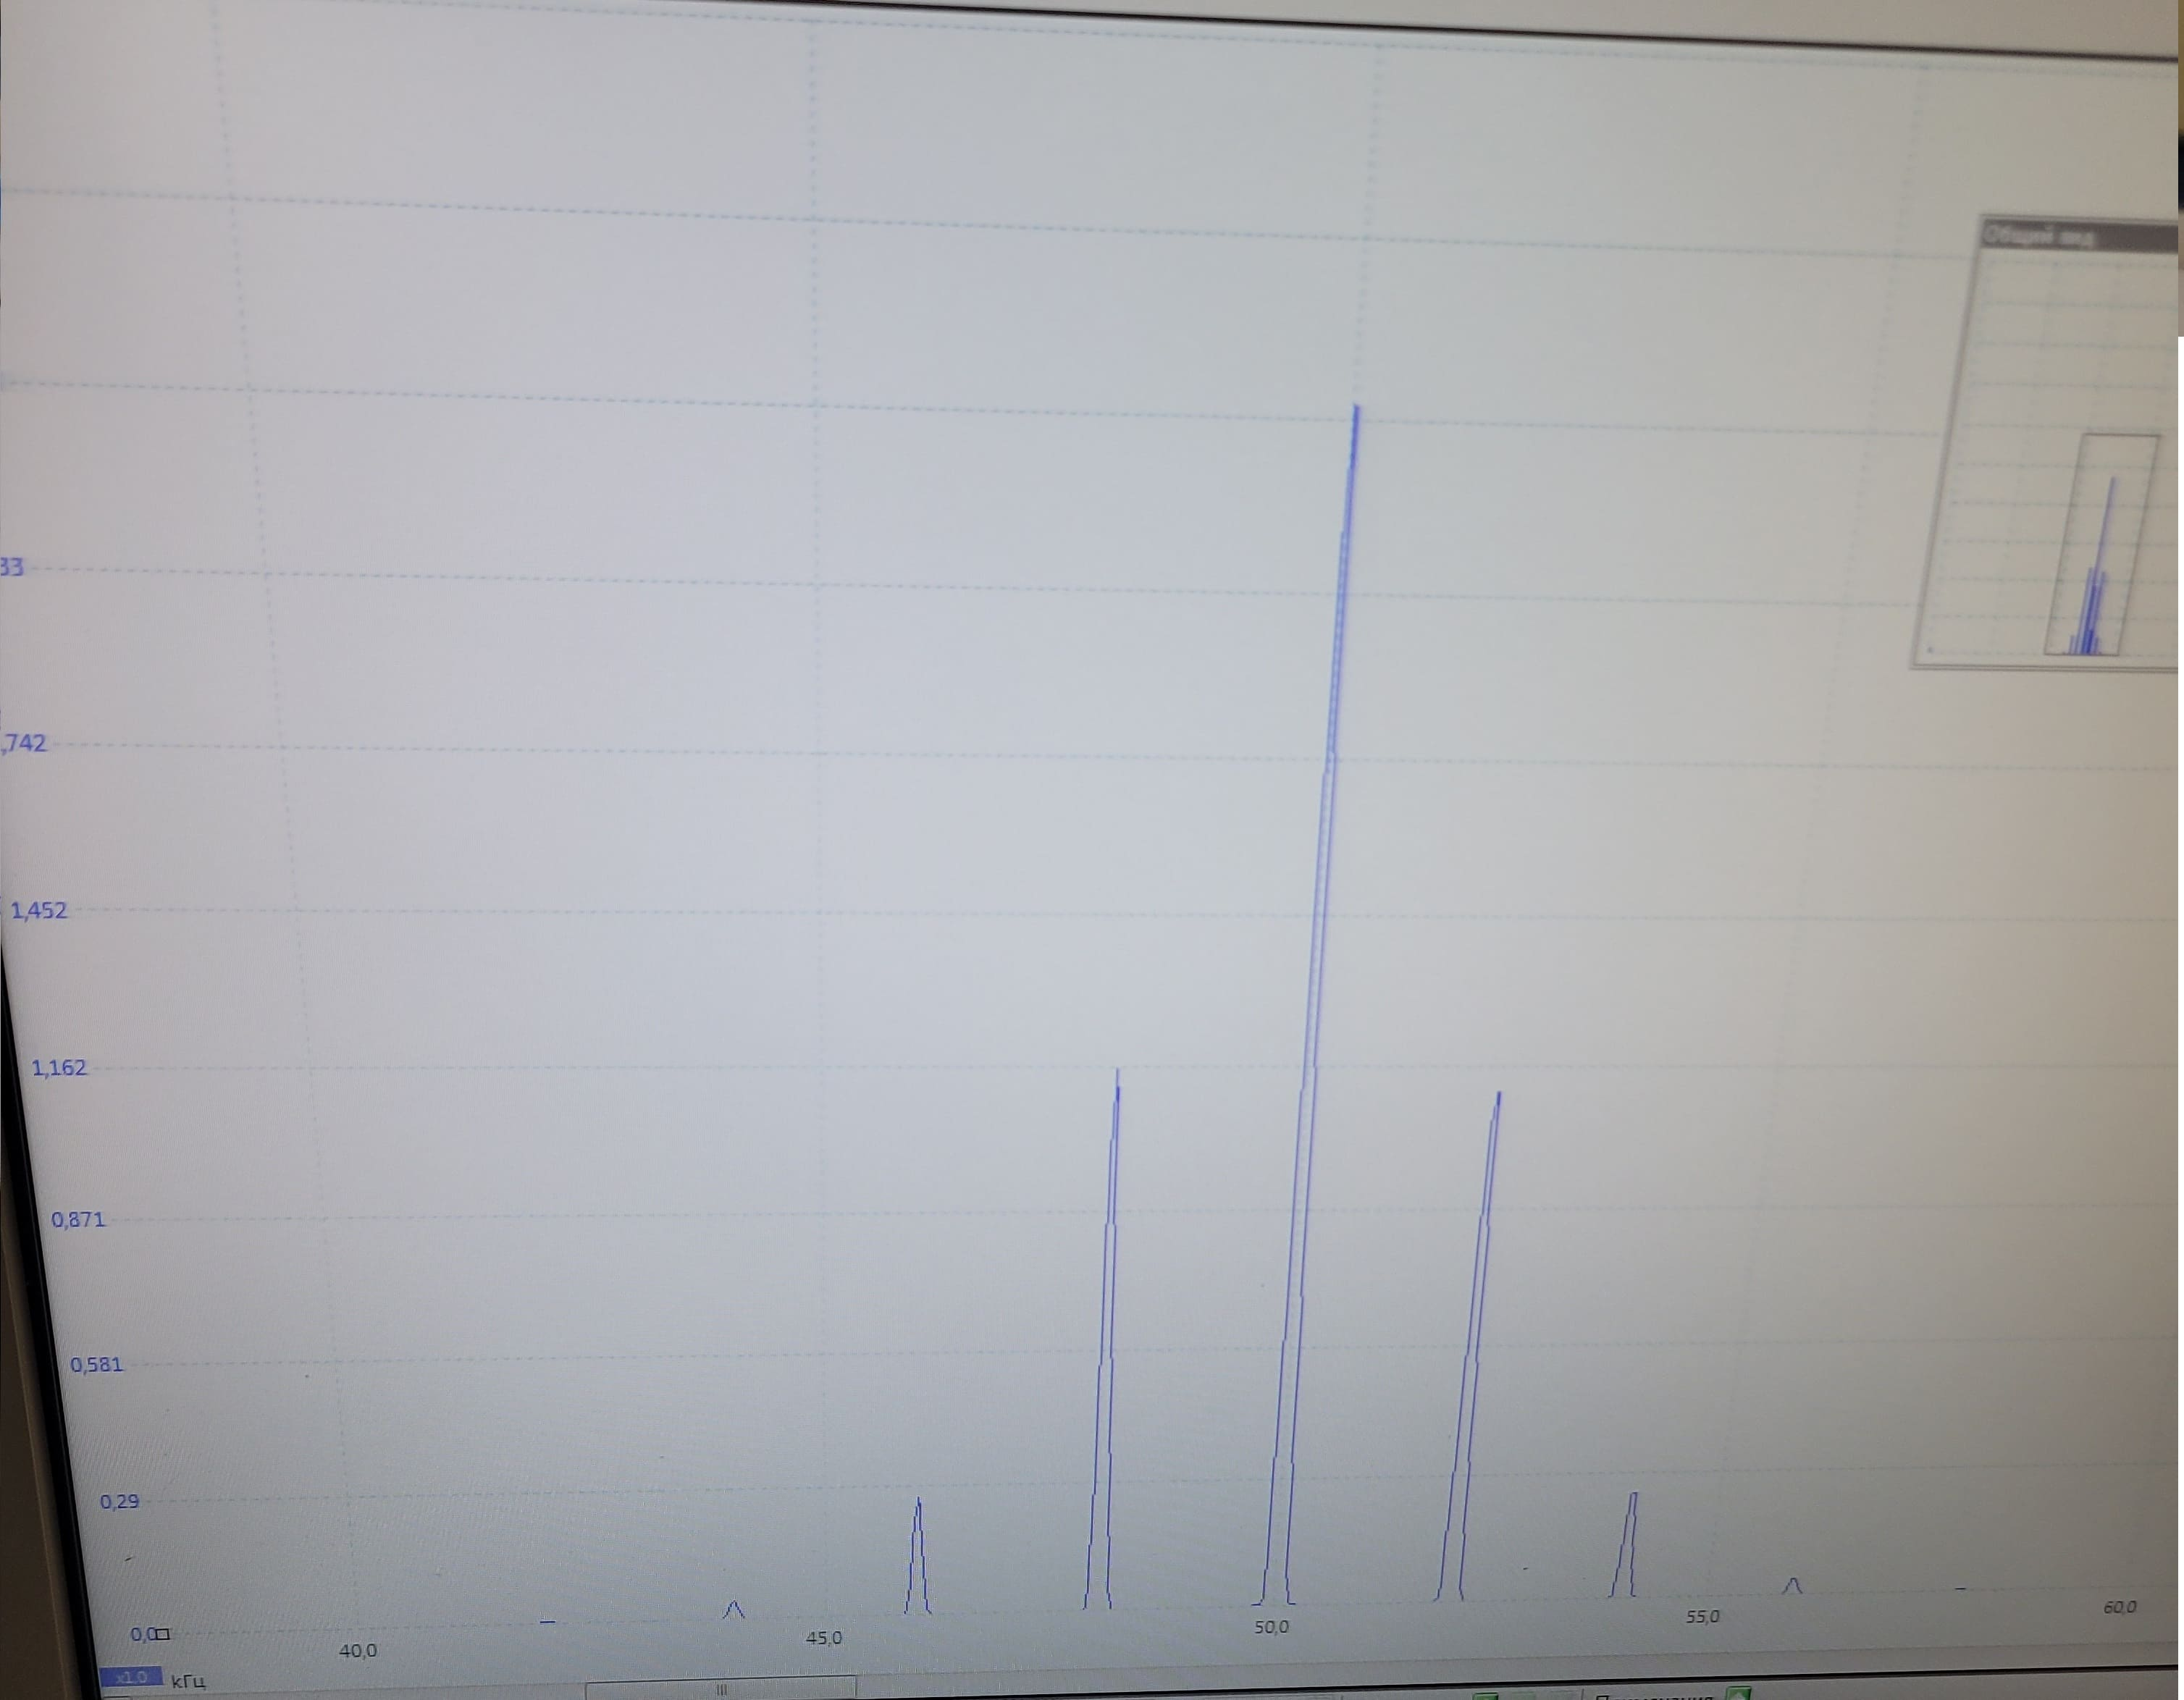
\includegraphics[width=1\linewidth]{D_50k_2k_50f.jpg}} $\nu_0$ = 50 кГц, $\nu_\text{мод}$ = 2 кГц, $\varphi$ = 50$\degree$   \\
\end{minipage}
\hfill
\begin{minipage}[h]{0.44\linewidth}
\center{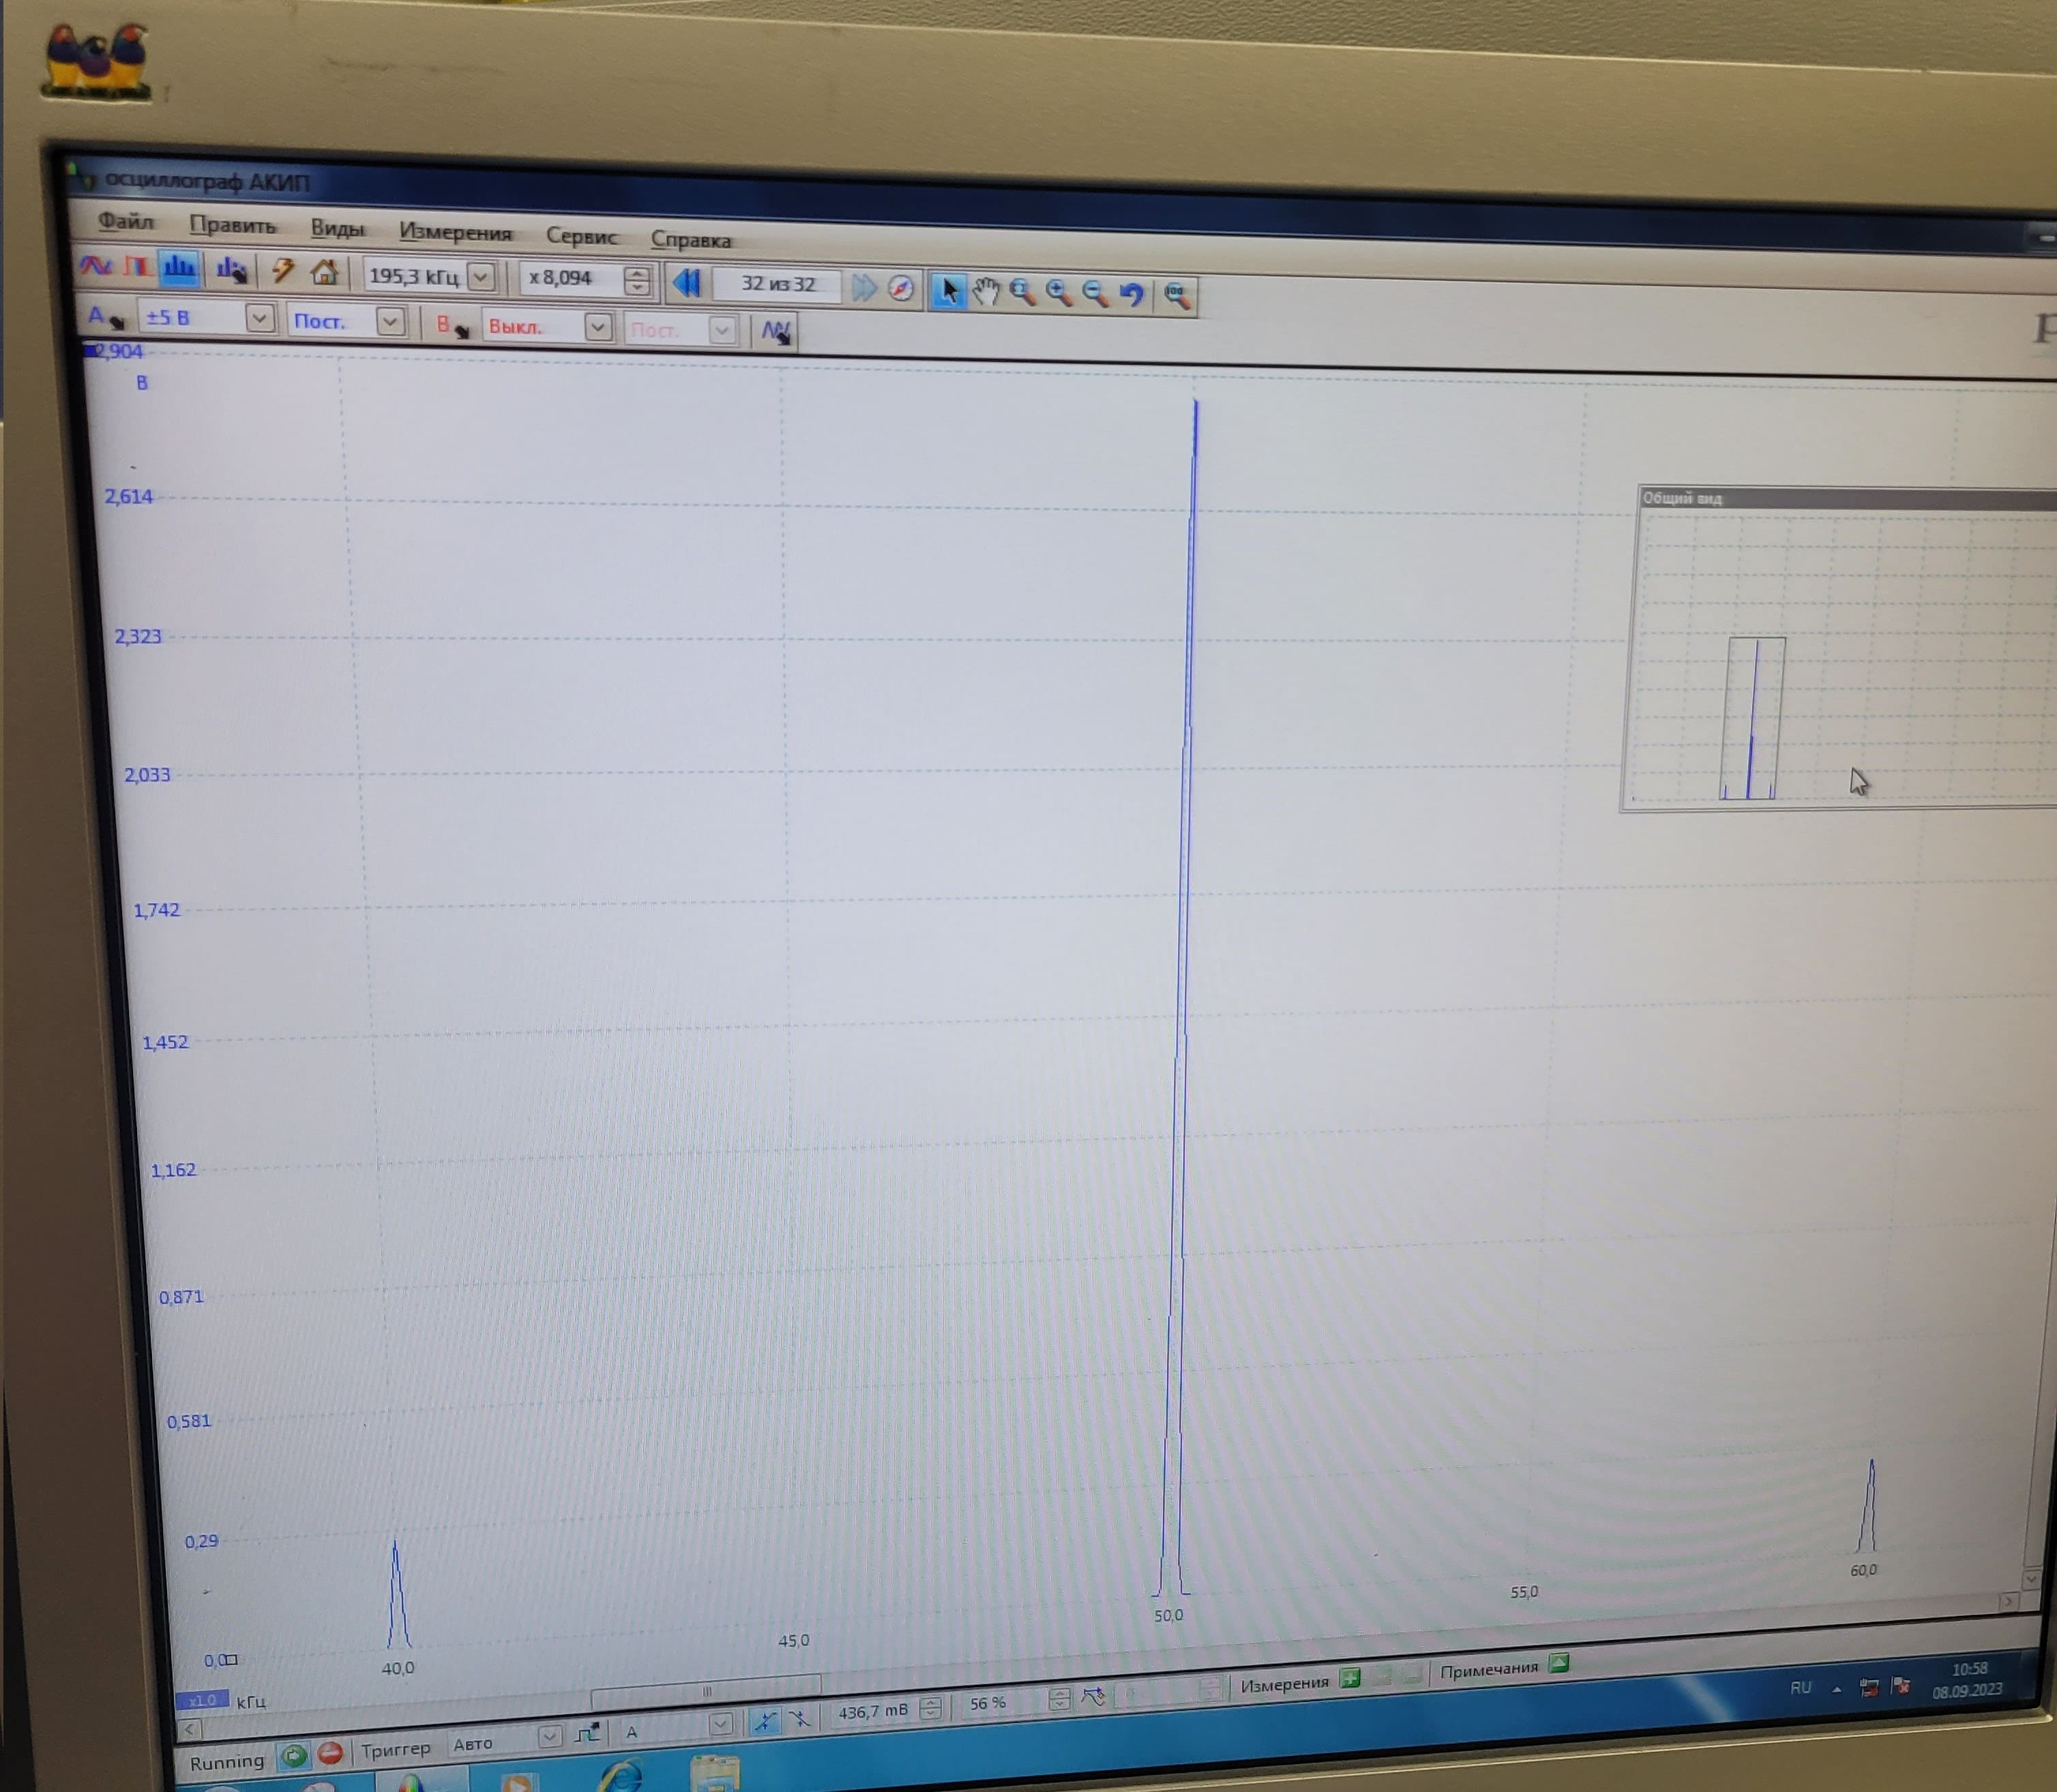
\includegraphics[width=1\linewidth]{D_50k_10k_10f.jpg}} $\nu_0$ = 50 кГц, $\nu_\text{мод}$ = 10 кГц, $\varphi$ = 10$\degree$  \\
\end{minipage}
\vfill
\caption{}
\label{ris:experimentalcorrelationsignals}
\end{figure}


\newpage




\begin{figure}[h]
\begin{minipage}[h]{0.44\linewidth}
\center{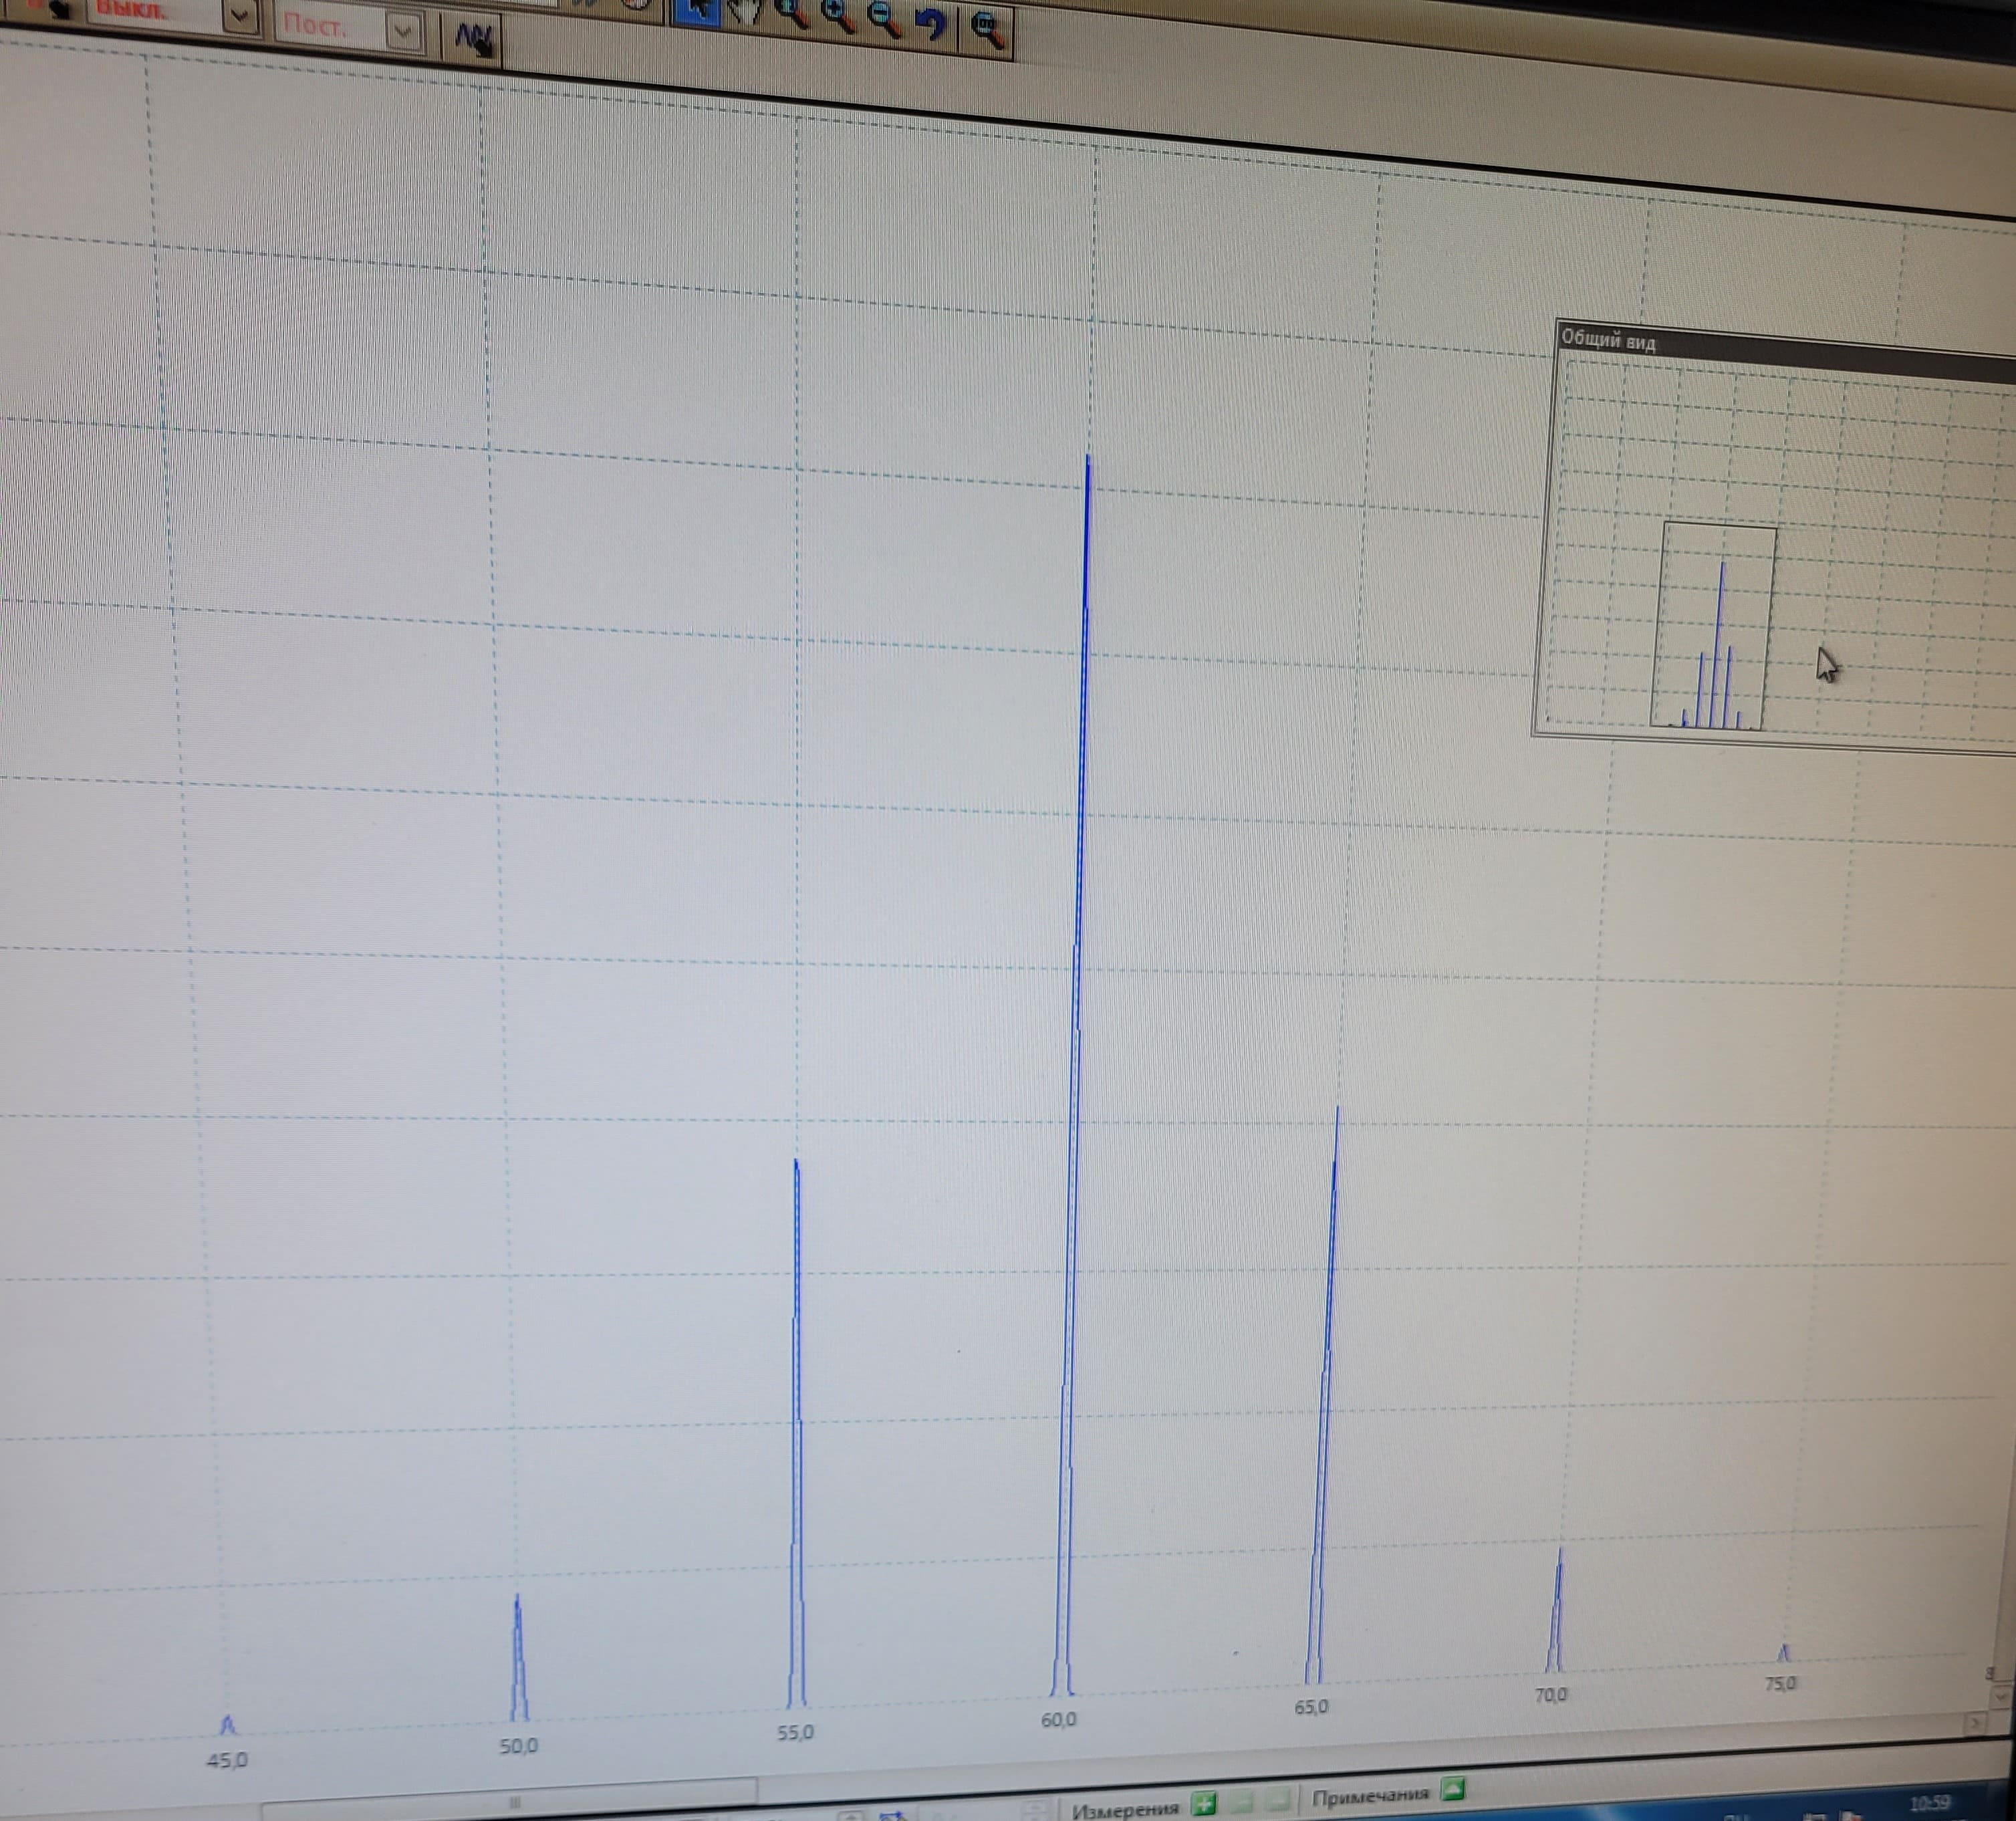
\includegraphics[width=1\linewidth]{D_60k_5k_50f.jpg}} $\nu_0$ = 60 кГц, $\nu_\text{мод}$ = 5 кГц, $\varphi$ = 50$\degree$  \\
\end{minipage}
\label{ris:experimentalcorrelationsignals}
\end{figure}




\end{enumerate}


\newpage










\subsection*{Е. Изучение фильтрации сигналов}



\begin{enumerate}


\item [\textbf{1.}] Подключаем $RC$ цепочку с сопротивлением $R = 3$ кОм и ёмкостью $C = 1000$ пФ. Получаем характерное время $\tau_{RC} = RC = 3 $ мкс. Подаём на вход $RC$-цепочки последовательность прямоугольных импульсов с периодом повторения $T \sim \tau_{RC}$.


\item [\textbf{2.}] Получаем на экране спектр (Преобразование Фурье) сигнала.

\begin{figure}[h]
\begin{minipage}[h]{0.44\linewidth}
\center{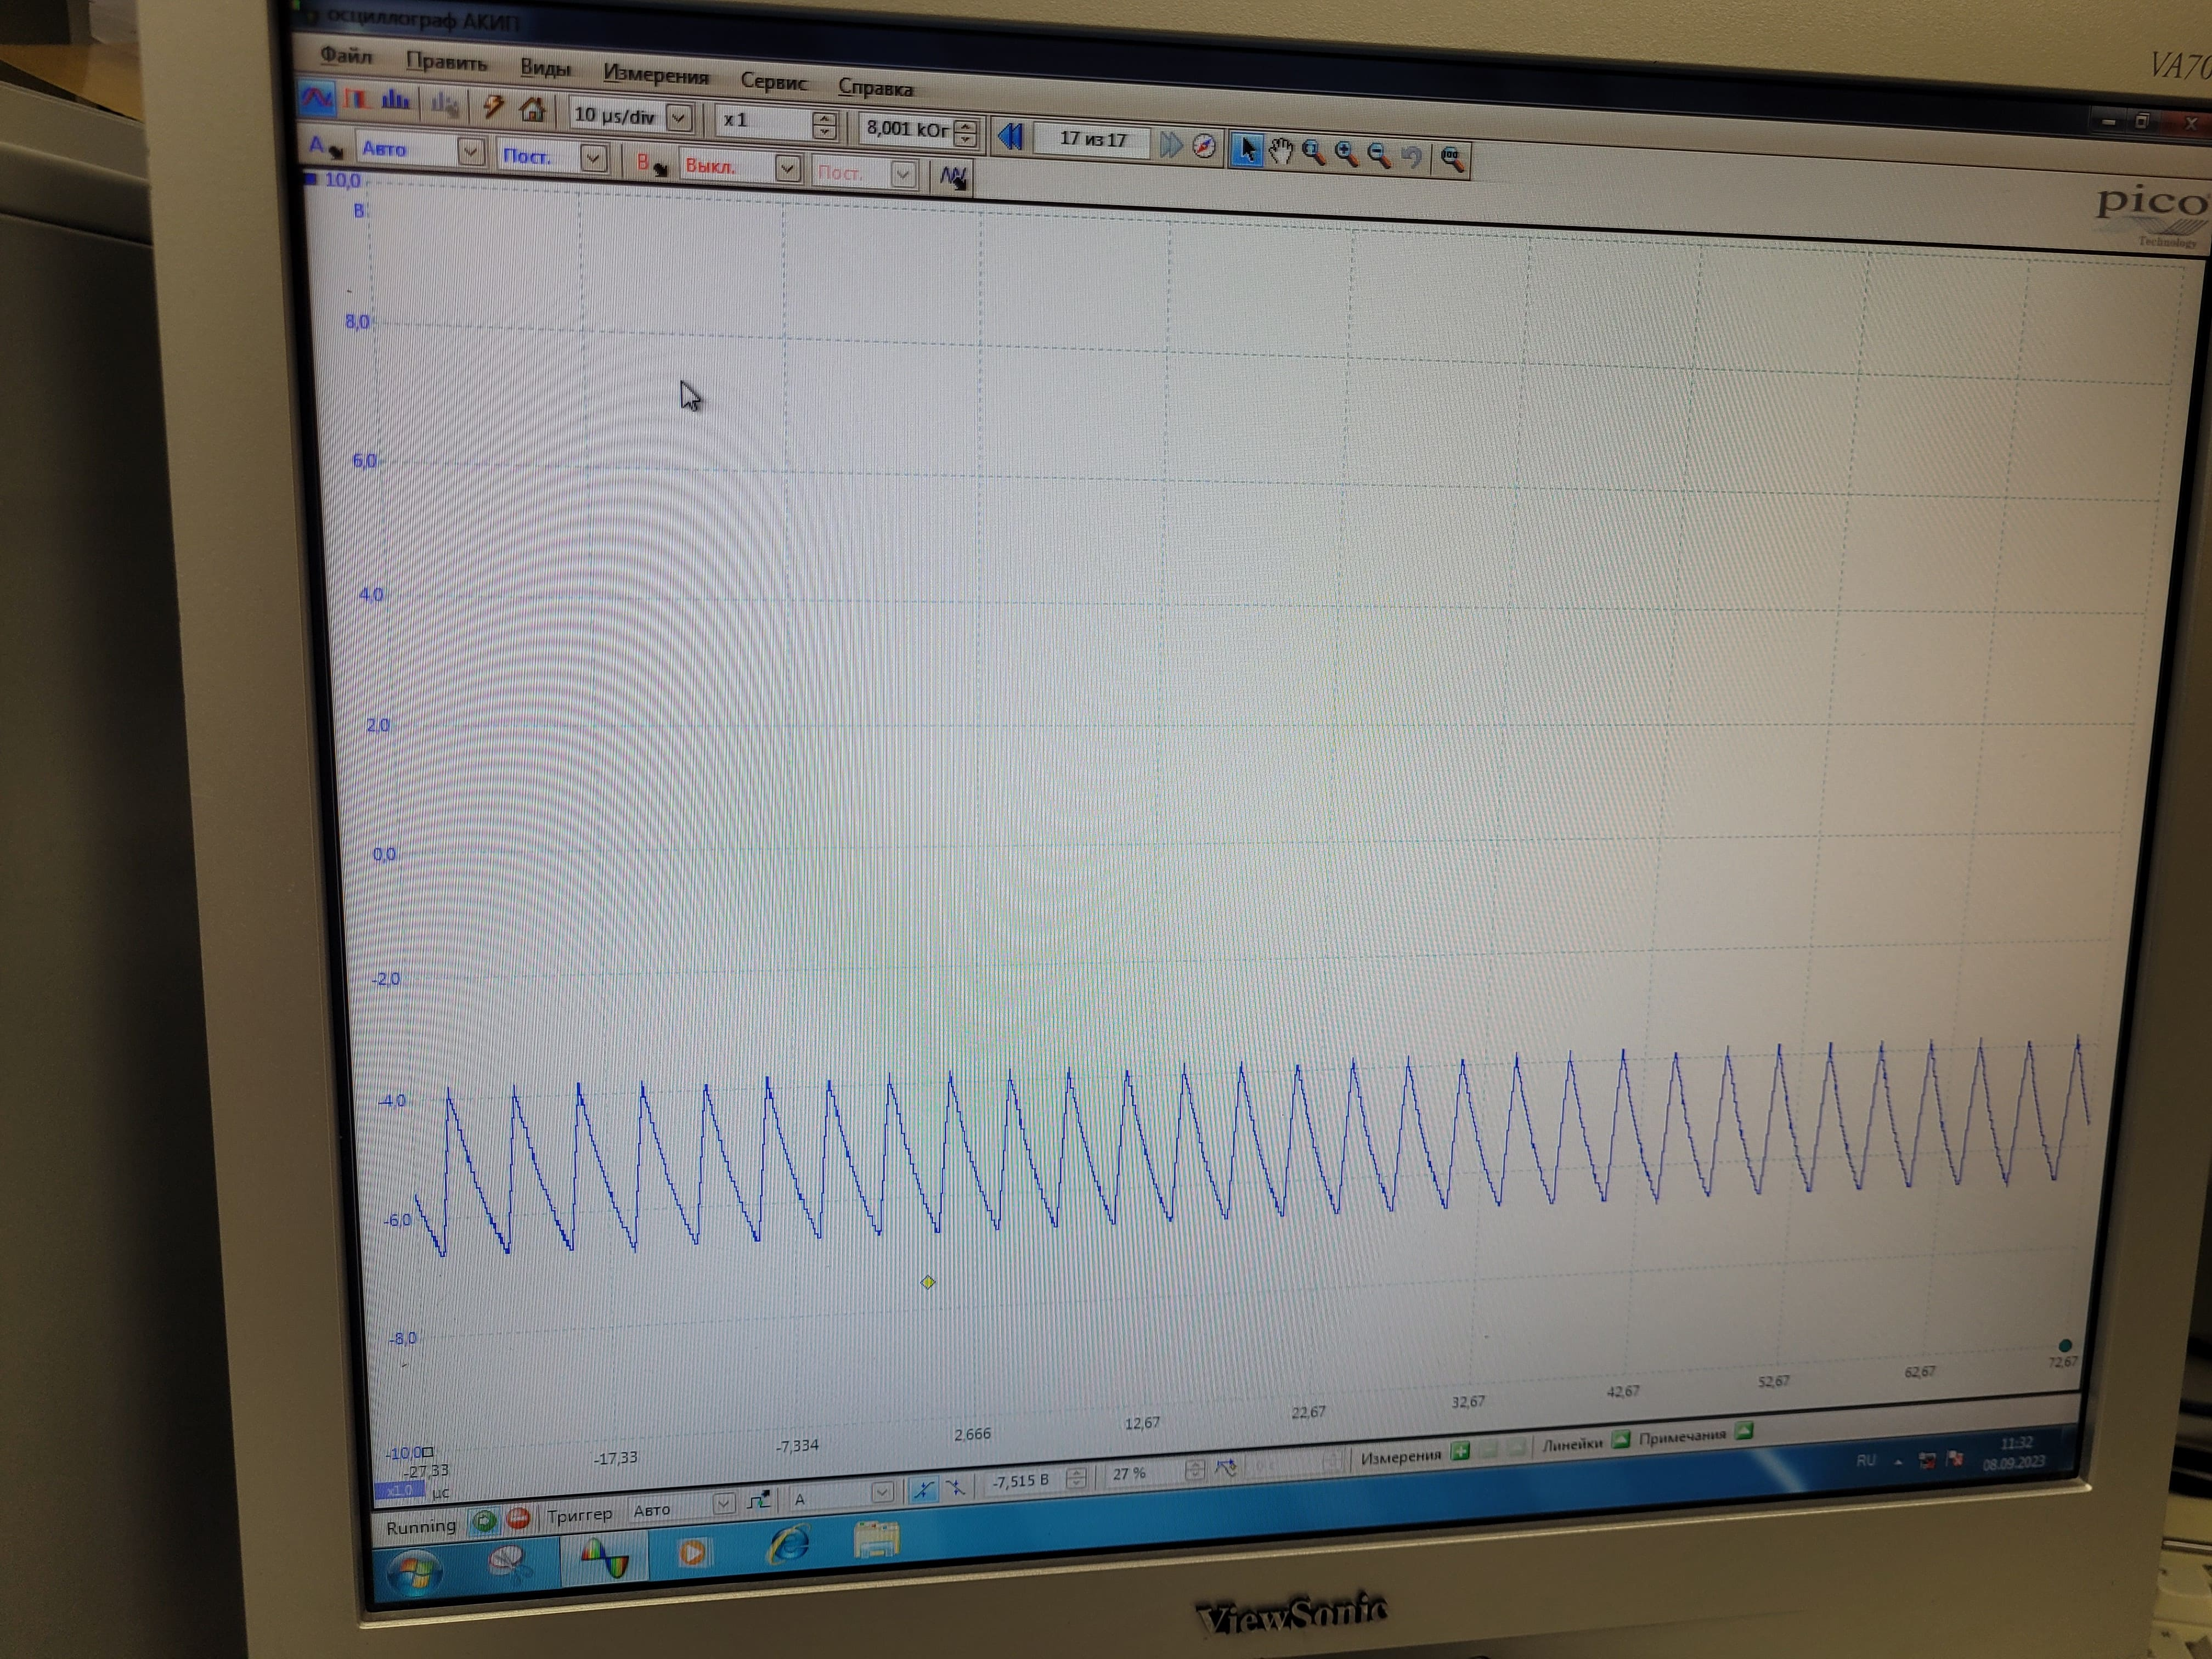
\includegraphics[width=1\linewidth]{E_sign_300k_510ns.jpg}} Сигнал при $\nu_0 = $ 300 кГц и $\tau$ = 510 нс.  \\
\end{minipage}
\hfill
\begin{minipage}[h]{0.44\linewidth}
\center{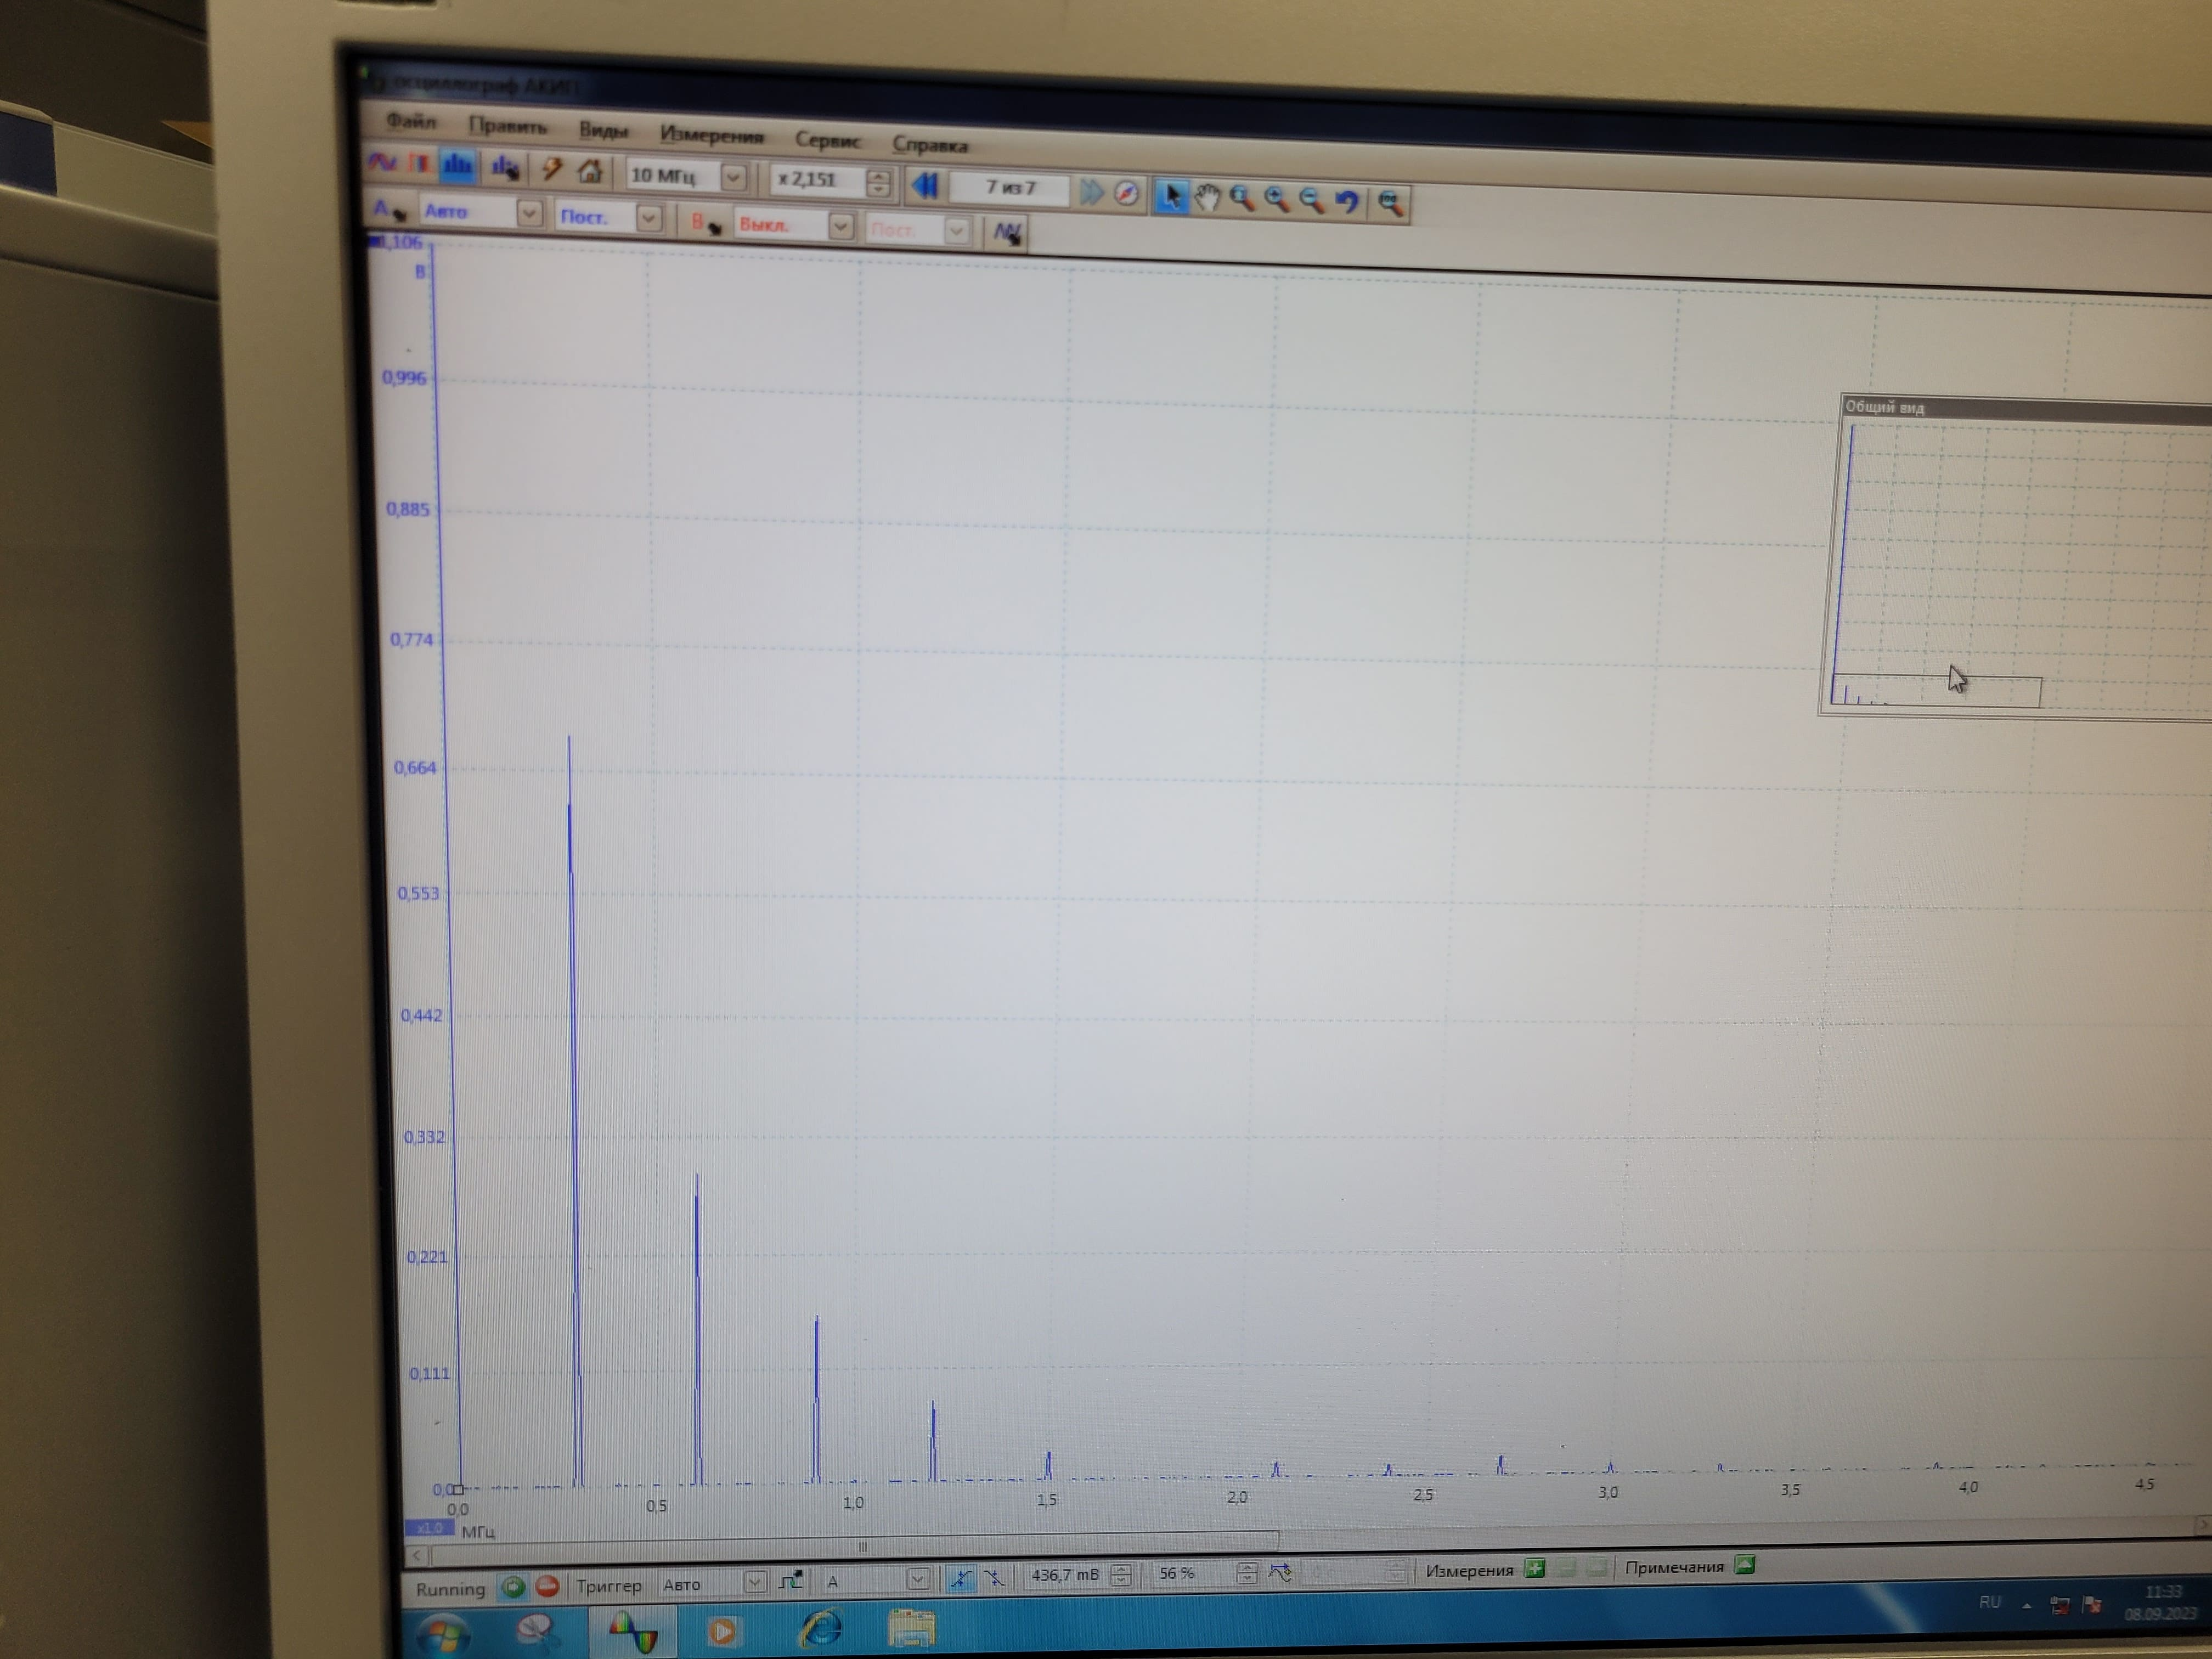
\includegraphics[width=1\linewidth]{E_spectr_300k_510ns.jpg}} \\  Спектр при $\nu_0 = $ 300 кГц и $\tau$ = 510 нс.
\end{minipage}
\vfill
\begin{minipage}[h]{0.44\linewidth}
\center{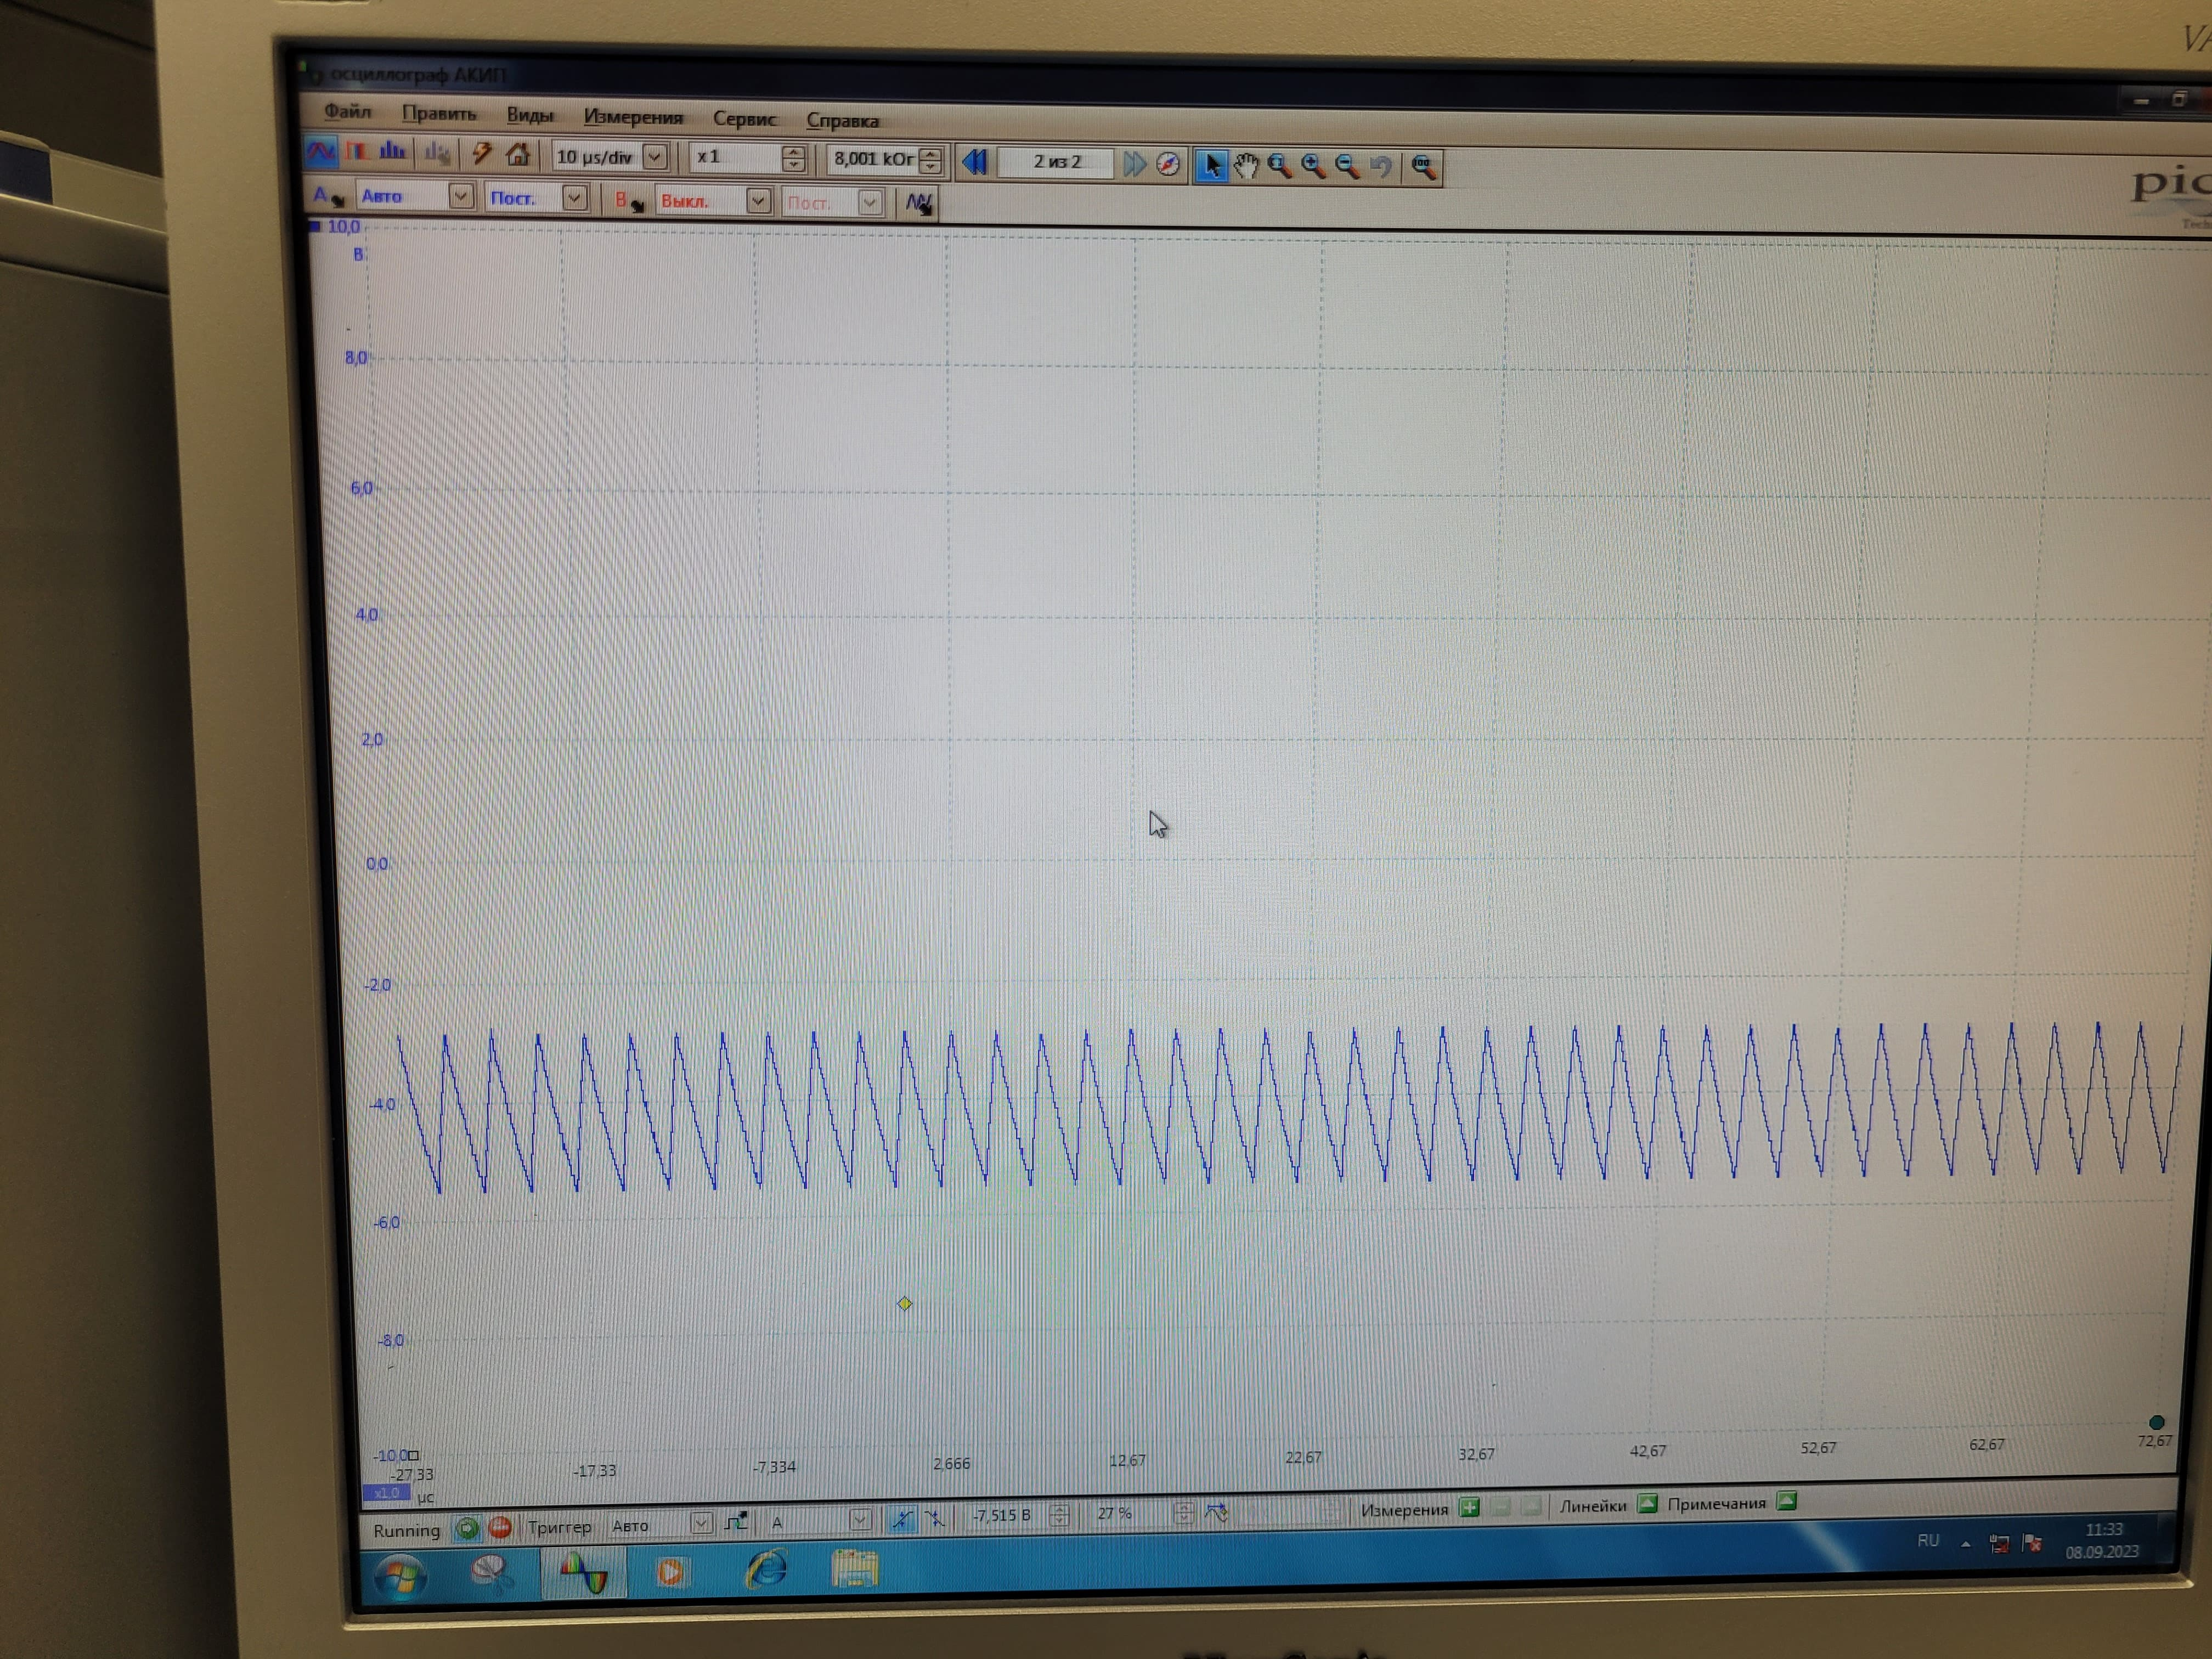
\includegraphics[width=1\linewidth]{E_sign_400k_510ns.jpg}} Сигнал при $\nu_0 = $ 400 кГц и $\tau$ = 510 нс.  \\
\end{minipage}
\hfill
\begin{minipage}[h]{0.44\linewidth}
\center{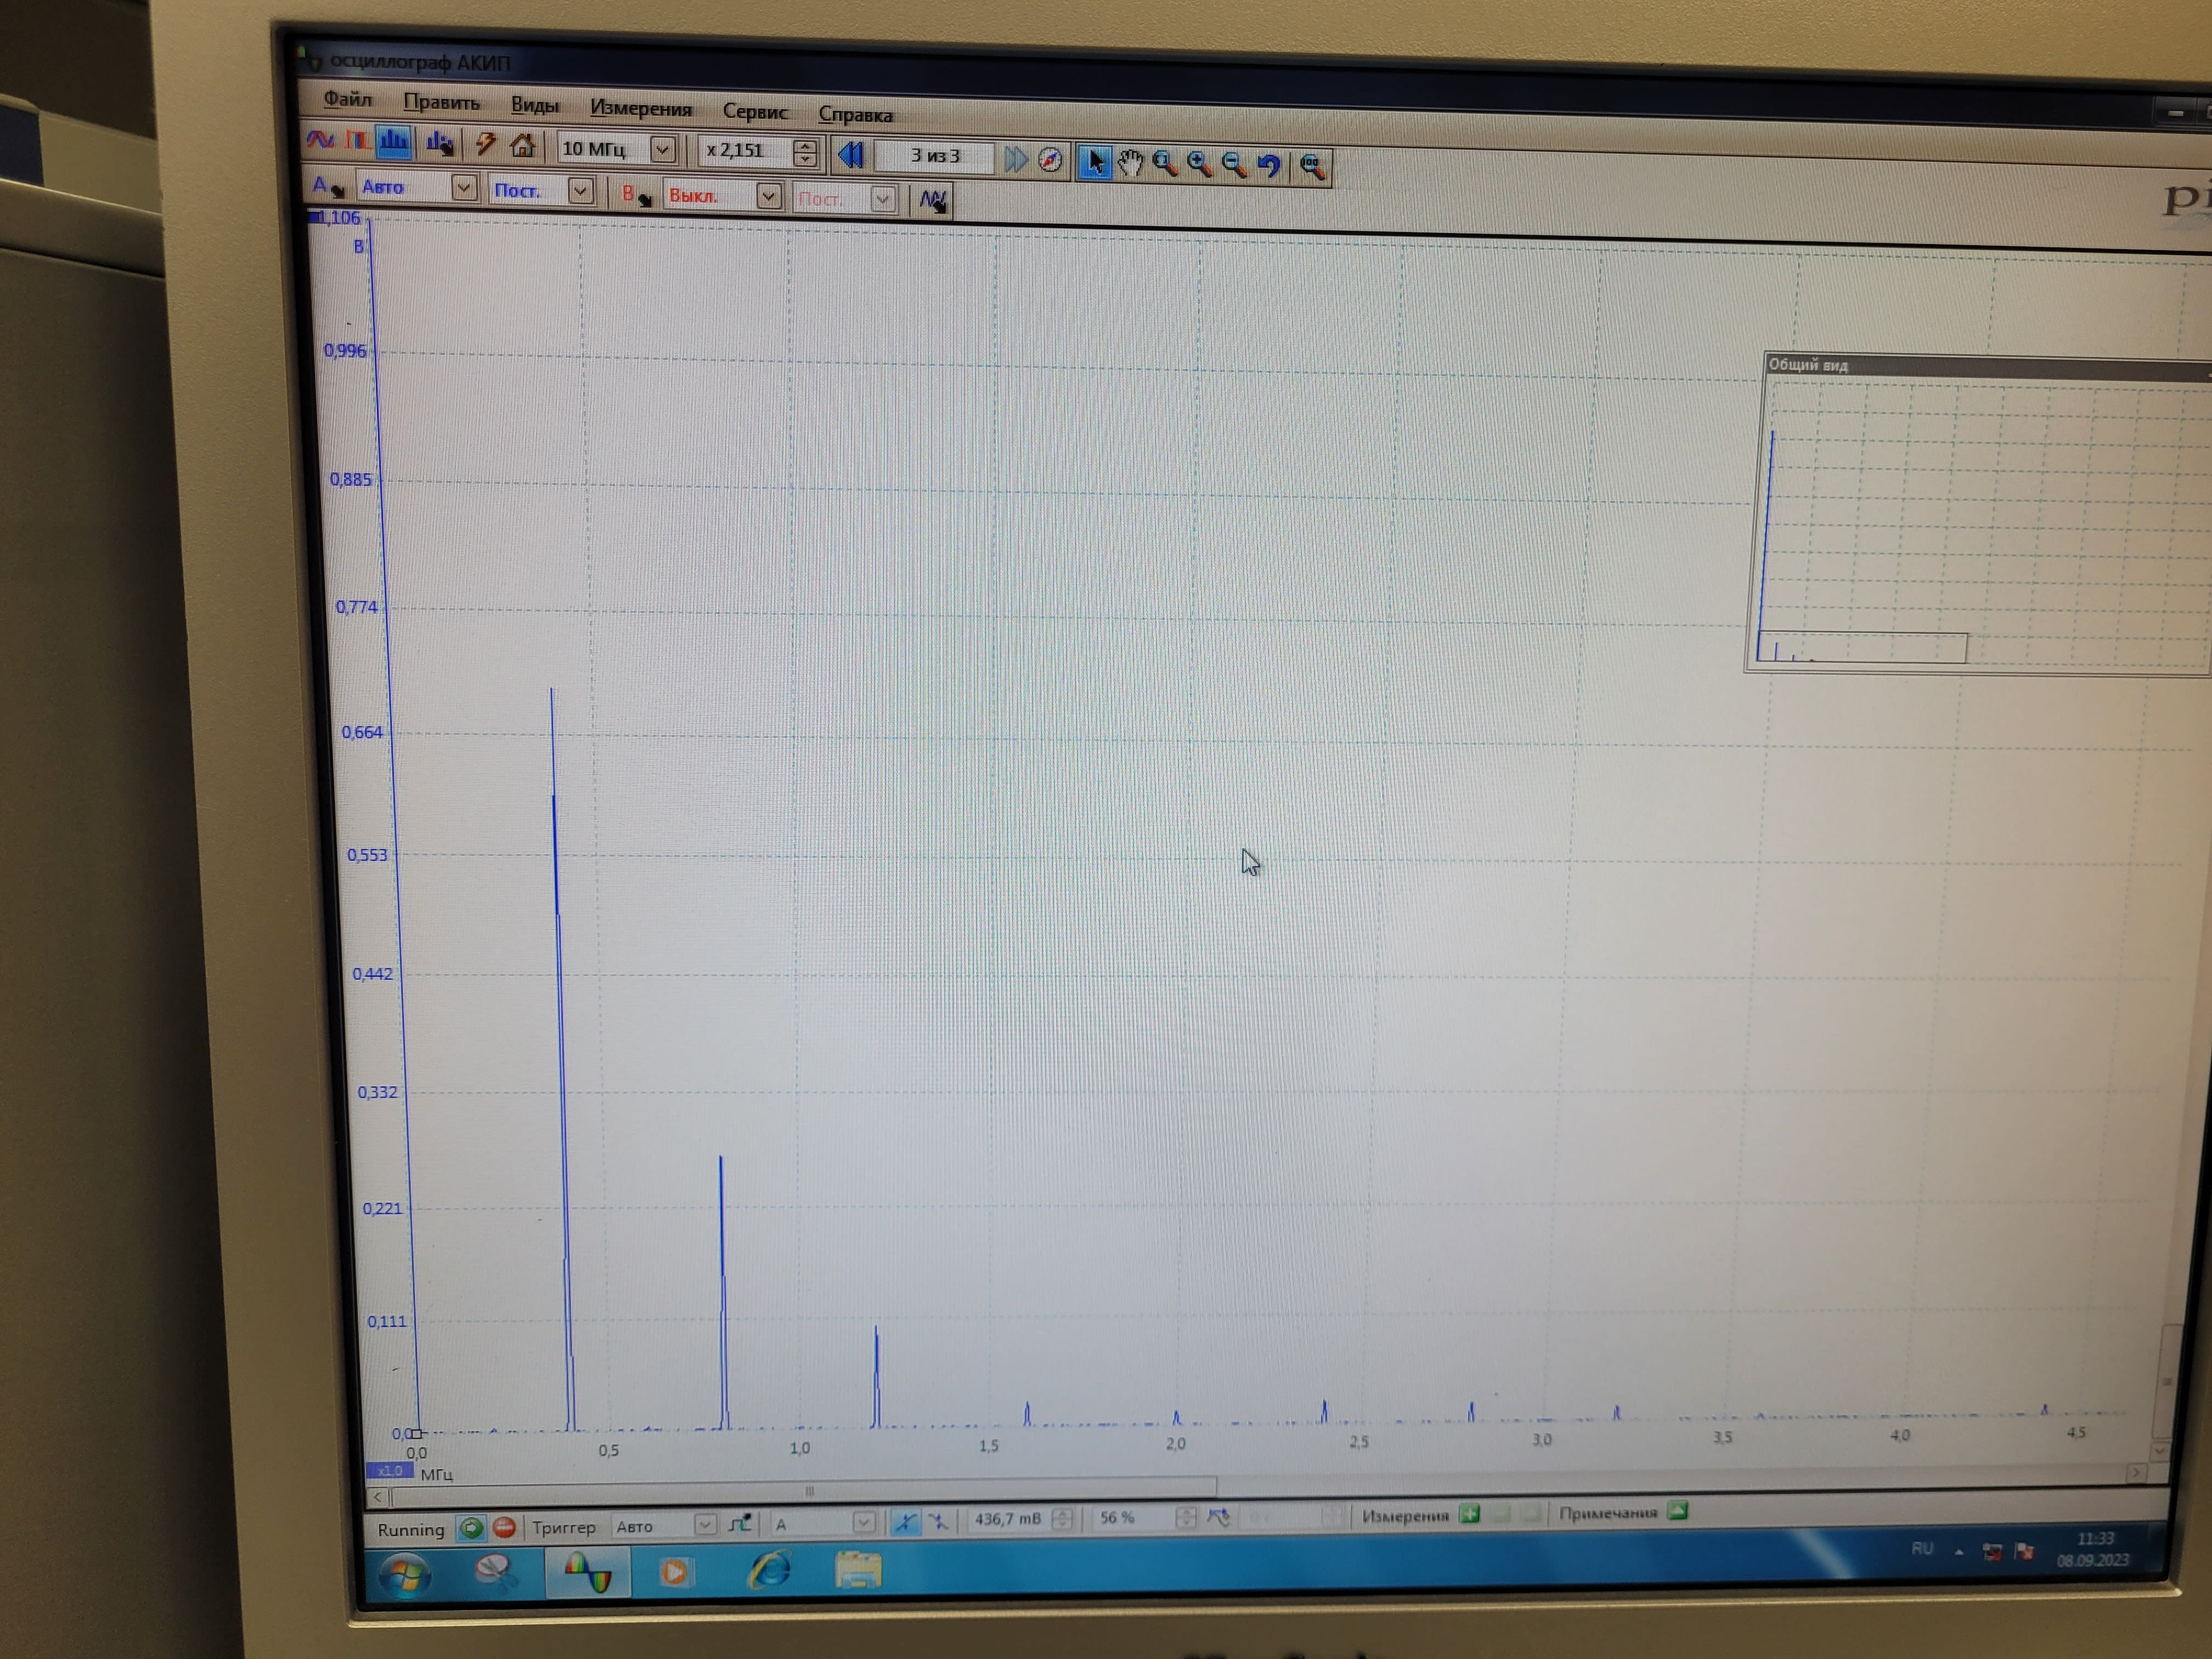
\includegraphics[width=1\linewidth]{E_spectr_400k_510ns.jpg}} Спектр при $\nu_0 = $ 400 кГц и $\tau$ = 510 нс. \\
\end{minipage}
\vfill
\caption{}
\label{ris:experimentalcorrelationsignals}
\end{figure}

\item [\textbf{3.}]
При фиксированной частоте $\nu = 300$ кГц проведем измерения отношений амплитуд соответствующих спектральных гармоник (для 7–9 гармоник) фильтрованного и исходного сигналов: $K_n = |a_n^\text{ф}|/|a_n^0|$. Для измерения
амплитуд $a_n^0$ спектра исходного сигнала переподключим генератор к осциллографу напрямую.

\begin{table}[h!]
    \centering
    \begin{tabular}{|c|c|c|c|c|c|c|c|c|c|}
\hline
$n$ & 1 & 2 & 3 & 4 & 5 & 6 & 7 & 8 & 9 \\ \hline
$a_n^\text{ф}$, мВ & 695.0 & 295.4 & 166.6 & 82.17 & 27.76 & 0 & 15.55 & 12.28 & 19.15 \\ \hline
$a_n^0$, мВ & 4452 & 3768 & 3151 & 1991 & 891 & 0 & 647 & 897 & 1008 \\ \hline
$K_n = |a_n^\text{ф}|/|a_n^0|$ & 0.156 & 0.078 & 0.0529 & 0.041 & 0.031 & ? & 0.024 &0.014 & 0.019 \\ \hline
\end{tabular}
    \caption{}
    \label{table4}
\end{table}

Построим график зависимости амплитудного коэффициента фильтрации $K(\nu)$ от частоты $\nu = n\nu_0$.
\begin{figure}[h]
    \centering
    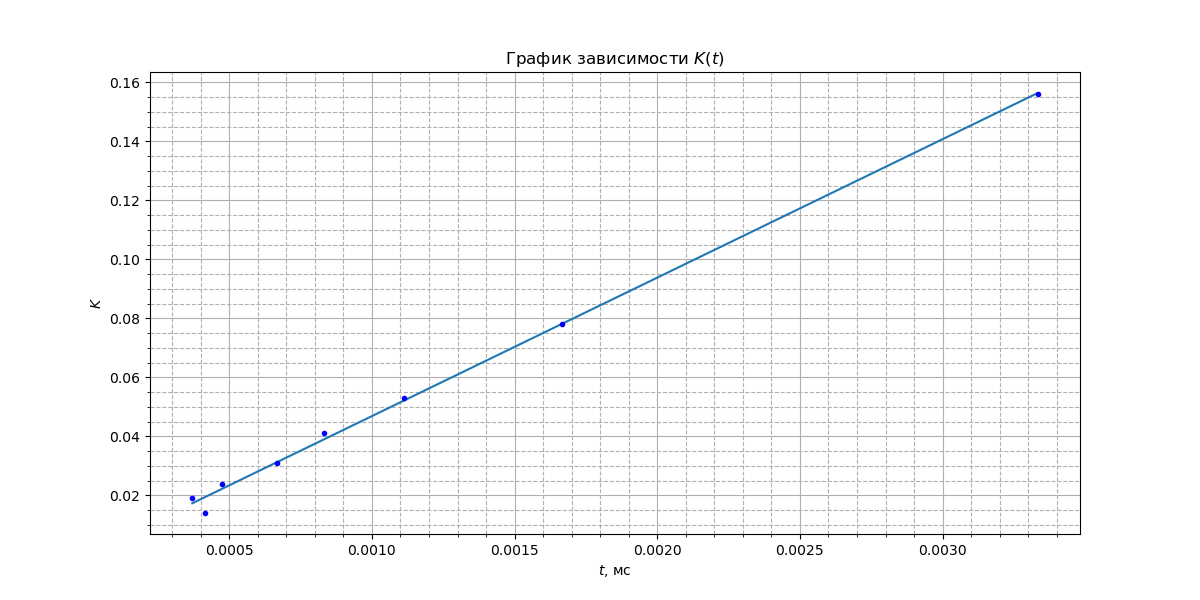
\includegraphics[width=\textwidth]{K(nu).png}
    \caption{Зависимость $K(\nu)$}
    \label{grafic3}
\end{figure}





Проверим, что экспериментальная зависимость
совпадает с теоретической $K = \frac{1}{\tau_\text{RC}} \int_0^t f(t')dt'$. Т.к. мы подаём последовательность прямоугольных импульсов, то права часть зависит линейно от $t$, т.е. обратно пропорционально $\nu$. График соответствует этой зависимости









\end{enumerate}



\newpage


\section*{Вывод}
В данной работе мы изучили понятие спектра и спектрального анализа, а также исследовали спектральный состав периодических электрических сигналов.

А именно, мы посмотрели на прямоугольные импульсы, цуги гармонических колебаний, а также гармонические сигналы, модулированные по амплитуде. Кроме того, нами был экспериментально проверен частный случай выполнения соотношения неопределённости.

\end{document}
